\chapter{Calibrazione}\label{ch:calibrazione}
Questo capitolo riguarda la parte di tesi incentrata sulla calibrazione delle centraline AirQino (\ref{sec:airqino}). Nella sezione \ref{sec:dati} vengono presentati i dataset a disposizione, la loro struttura e il lavoro di preprocessamento fatto.

La sezione \ref{sec:regressione} racchiude una breve panoramica teorica sui concetti di regressione, correlazione, metriche (coefficiente di correlazione, coefficiente di determinazione, scarto quadratico medio), analisi dei residui e modelli di regressione (sia lineare che non lineari).

La sezione \ref{sec:esperimenti} elenca gli esperimenti svolti per ciascun inquinante (\ce{NO2}, \ce{PM_{2.5}} e \ce{PM_{10}}) e presenta i risultati ottenuti (con analisi dei residui e confrontando i vari modelli, sia su tutto l'anno che mese per mese), mentre in \ref{sec:validazione} viene presentato il lavoro svolto per la validazione del modello di regressione migliore su un set di dati non visto in precedenza.

Infine, la sezione \ref{sec:discussione} riassume tutto il lavoro svolto e fornisce un'analisi qualitativa dei risultati ottenuti.

% I dati a disposizione
\clearpage
\section{Dati a disposizione}\label{sec:dati}
I dataset messi a disposizione sono due:

\begin{itemize}
  \item Dataset delle misurazioni di concentrazione di \ce{NO2} nell'aria relative alla centralina SMART16 AirQino, da confrontare con i dati \ce{NO2} ARPAT\footnote{Agenzia regionale per la protezione ambientale della Toscana} della stazione Capannori (Lucca);
  \item Dataset delle misurazioni di concentrazione di \ce{PM_{2.5}} e \ce{PM10} nell'aria relative alla centralina SMART16 AirQino, da confrontare con i dati \ce{PM_{2.5}} e \ce{PM10} ARPAT della stazione Capannori (Lucca).
\end{itemize}

In entrambi i casi la centralina SMART16 è stata in co-locazione con la stazione ARPAT di Capannori per tutto periodo di interesse.\\

\begin{figure}[H]
\centering
\captionsetup{justification=centering}
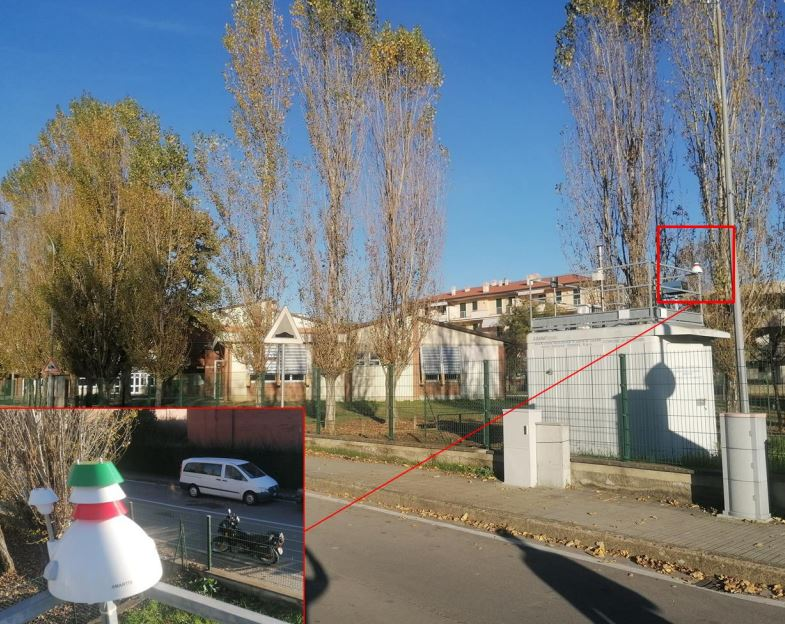
\includegraphics[width=0.75\textwidth,height=\textheight,keepaspectratio]{img/smart72.jpg}
\caption{Una centralina AirQino\\Fonte: \url{https://airqino.magentalab.it}}
\label{fig:smart72}
\end{figure}

\begin{figure}[H]
\centering
\captionsetup{justification=centering}
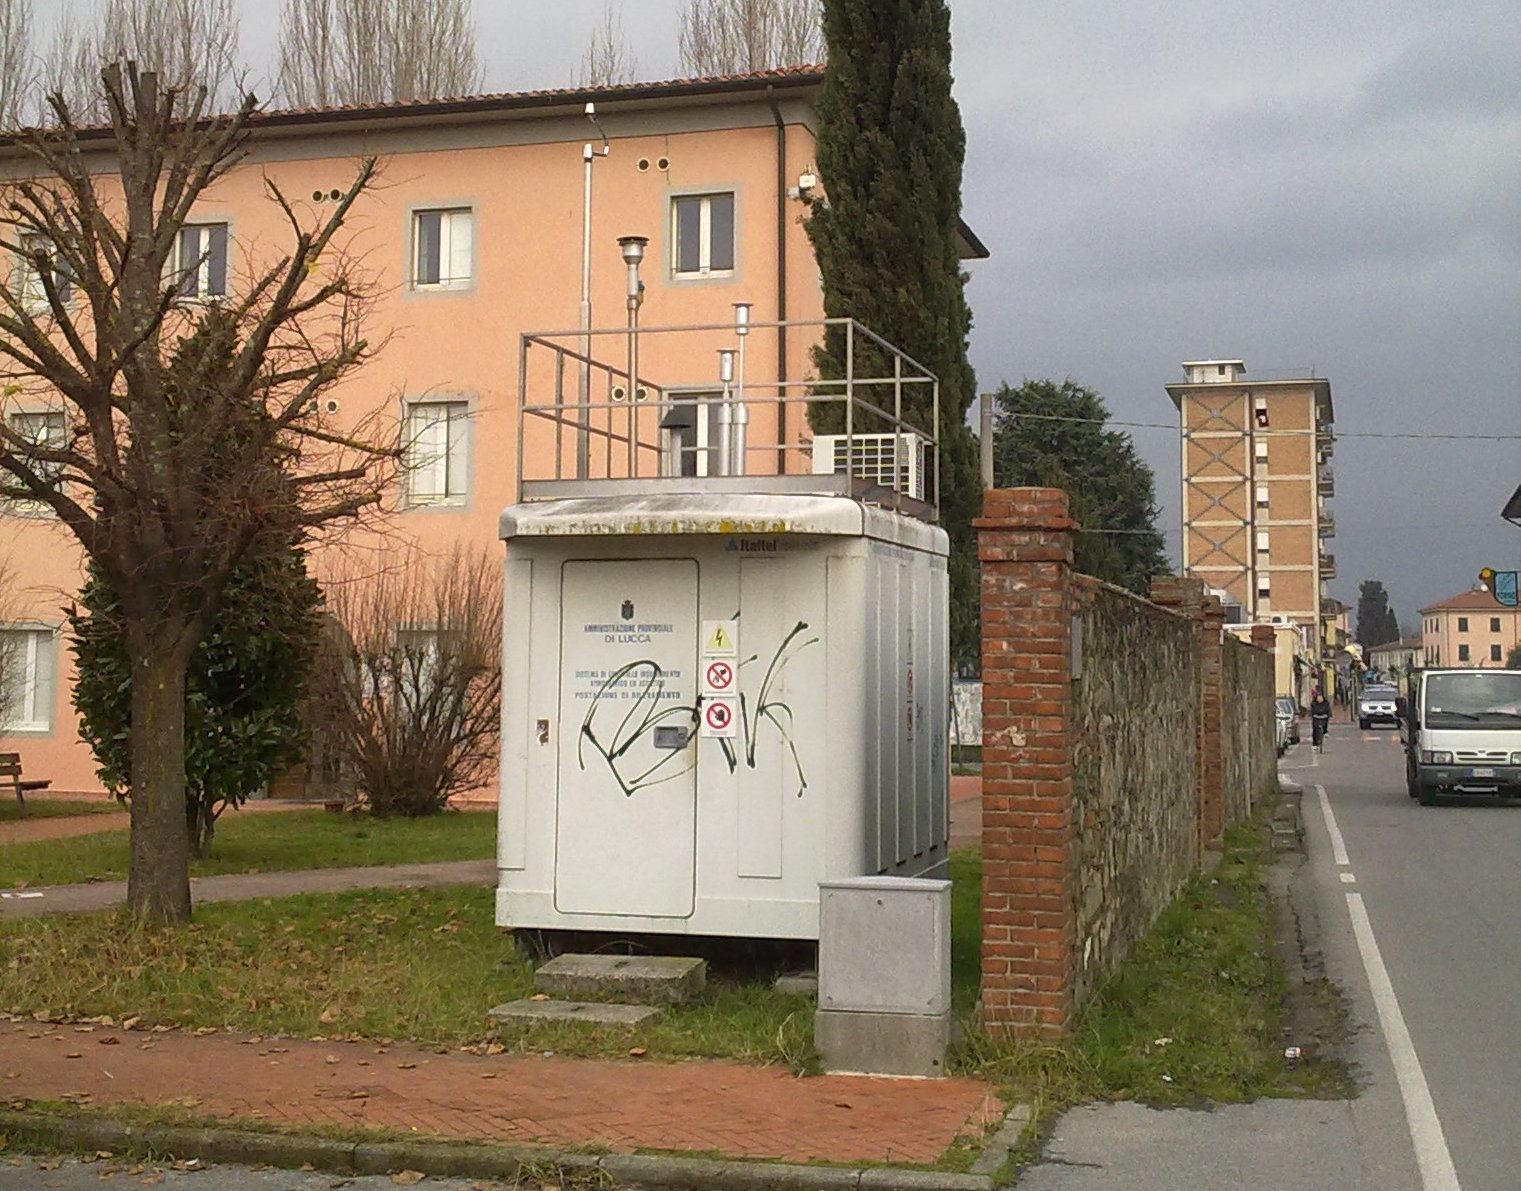
\includegraphics[width=0.75\textwidth,height=\textheight,keepaspectratio]{img/lu-capannori.jpg}
\caption{Centralina ARPAT in sede Capannori (provincia di Lucca)\\Fonte: \url{http://arpat.toscana.it}}
\label{fig:capannori}
\end{figure}

\begin{figure}[H]
\centering
\captionsetup{justification=centering}
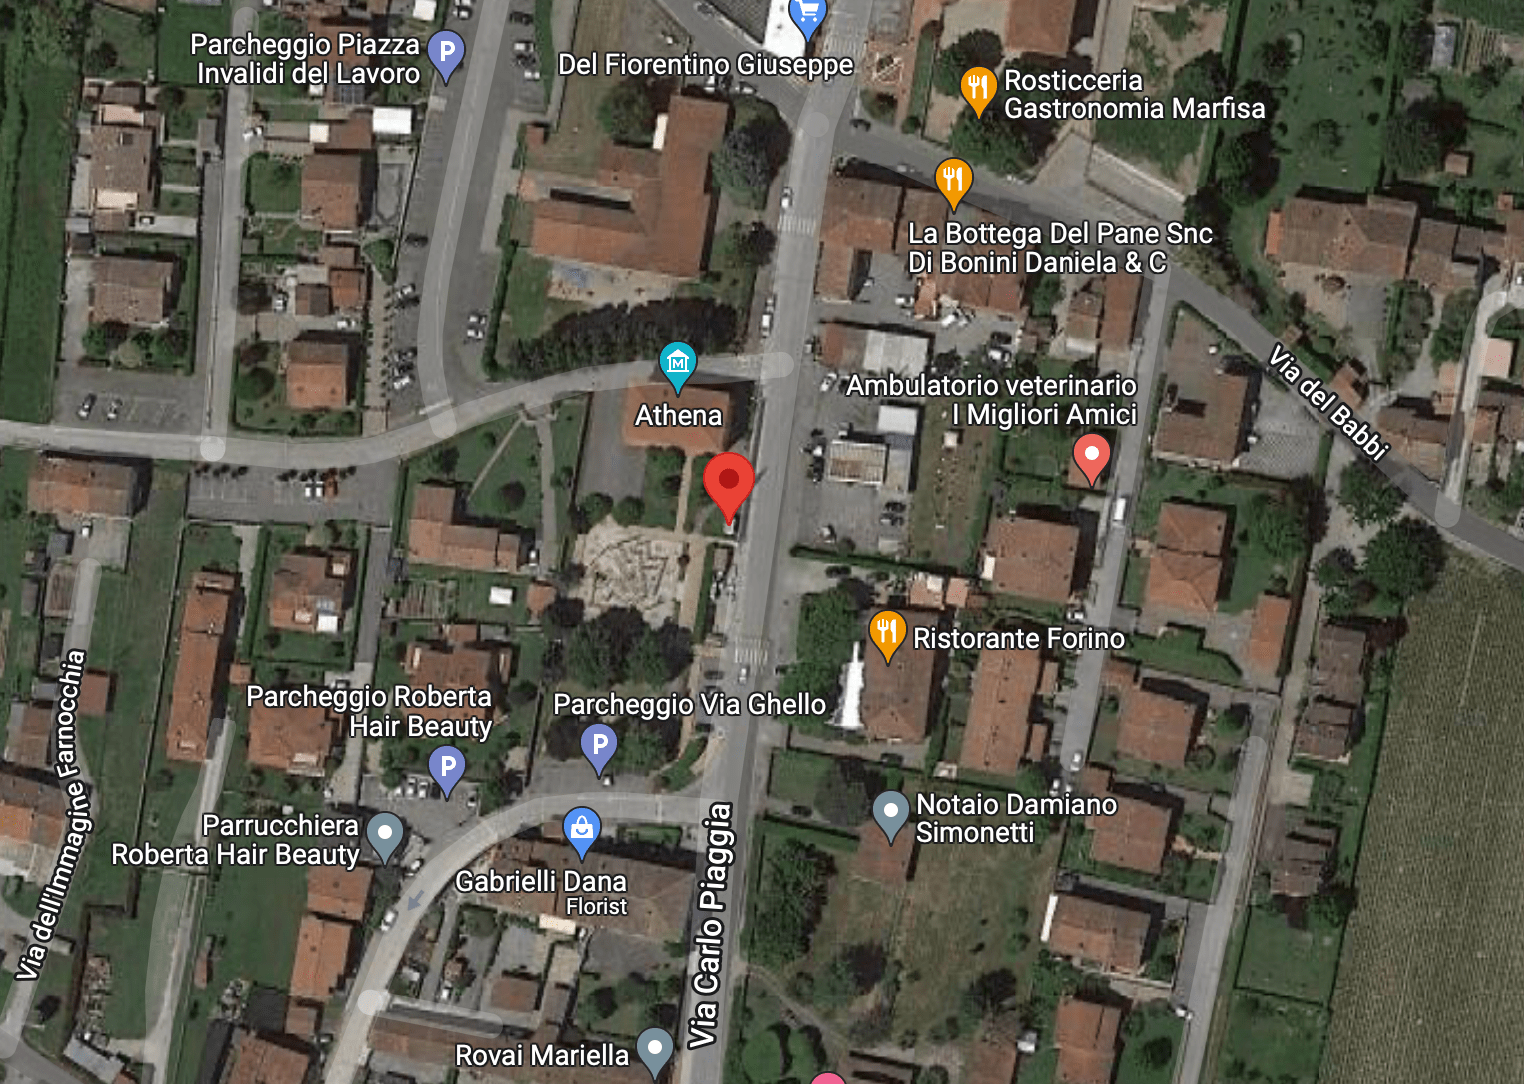
\includegraphics[width=0.75\textwidth,height=\textheight,keepaspectratio]{img/capannori_gps.png}
\caption{Posizione della centralina SMART16 (AirQino)\\e ARPAT (Capannori) a Lucca}
\label{fig:capannori-gps}
\end{figure}
\clearpage

\subsection{Dataset \ce{NO2}}\label{ssec:dataset-no2}
Il dataset di misurazioni \ce{NO2} comprende sia i dati della centralina AirQino SMART16 che i dati di ARPAT (Capannori). Ci sono però delle differenze sostanziali tra i due set di dati:\\

\begin{table}[H]
\centering
\def\arraystretch{0.9}
\begin{tabular}{|l|l|l|l|}
\cline{2-4}
\multicolumn{1}{c|}{} & \textbf{Periodo} & \textbf{Unità} & \textbf{Frequenza dati} \\ \hline
\textbf{SMART16} & 01/01/2020 - 31/12/2020 & \textit{counts} & ogni 1/2 minuti \\ \hline
\textbf{ARPAT} & 01/01/2020 - 31/12/2020 & µg/m³ & medie giornaliere \\ \hline
\end{tabular}
\caption{Differenze tra i dati di SMART16 e ARPAT (per \ce{NO2})}
\label{tab:dataset-no2-tabella}
\end{table}

Da notare che le centraline AirQino misurano la concentrazione di \ce{NO2} con il sensore \textbf{MiCS-2714} (come già accennato in \ref{ssec:hardware}) che fornisce output in \textit{counts} (unità di misura del segnale convertito da analogico a digitale, con uscita a 10 bit). Questo significa che sarà compito della fase di calibrazione convertire l'output direttamente in unità ingegneristica (in questo caso µg/m³).\\

Nella figura \ref{fig:smart16-no2} sono riportate la frequenza di misurazione (intesa come il numero di misurazioni effettuate ogni ora) e l'andamento della concentrazione di \ce{NO2} nell'aria (in \textit{counts}) per come sono state misurate dalla centralina SMART16 nel periodo di interesse (01/01/2020 - 31/12/2020).

La figura \ref{fig:arpat-no2} invece riporta l'andamento della concentrazione di \ce{NO2} nell'aria (in µg/m³) misurato dalla stazione ARPAT di Capannori nello stesso periodo.

\clearpage
\begin{figure}[H]%
    \centering
    \captionsetup{justification=centering}
    \subfloat[\centering Frequenza di misurazione]{{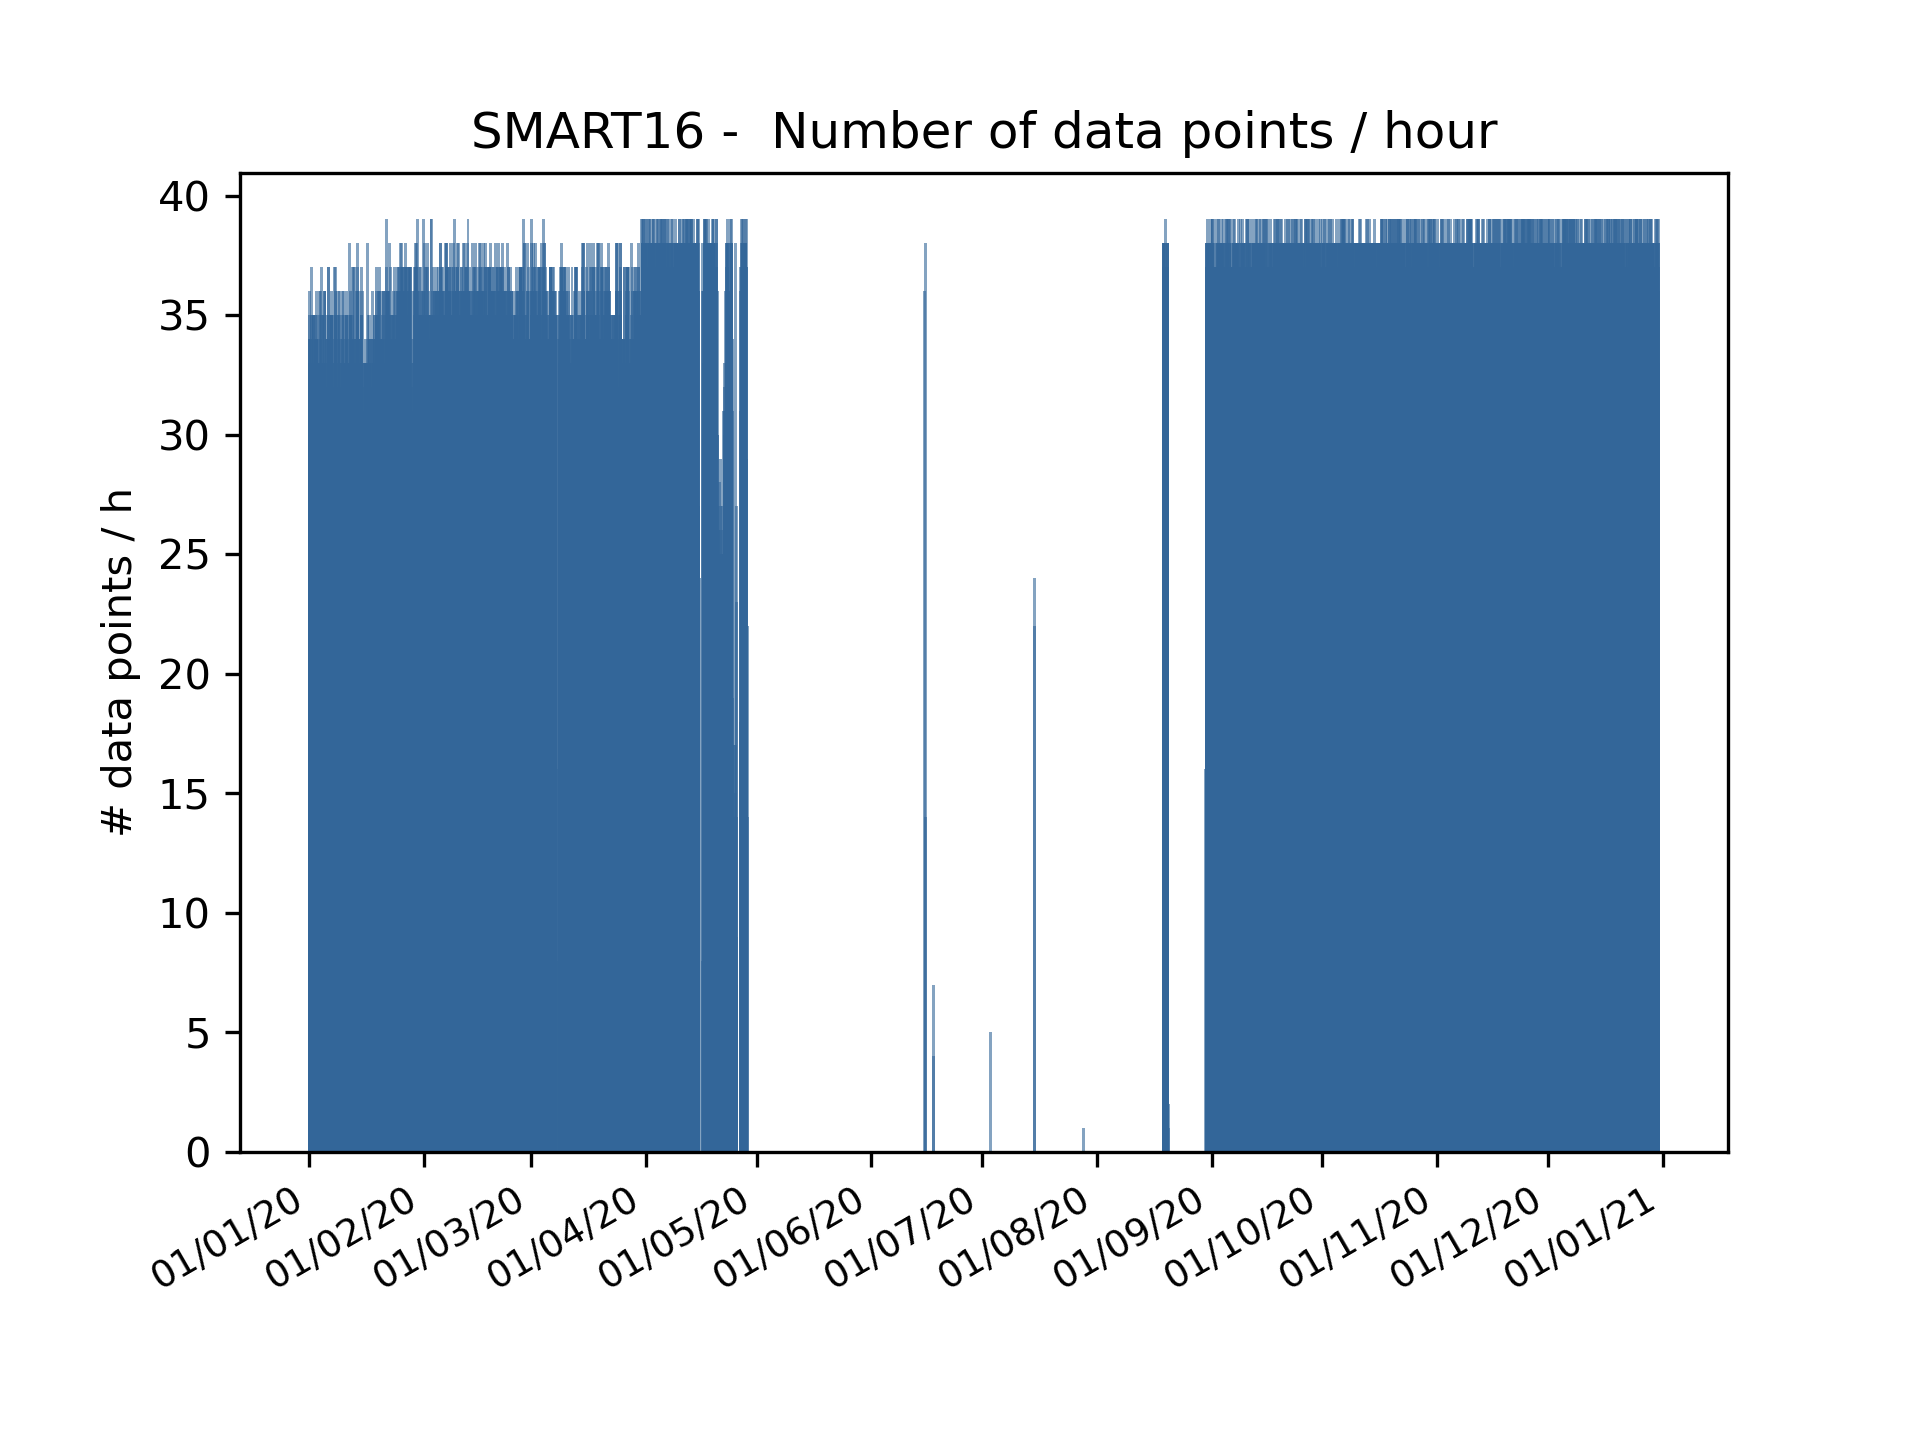
\includegraphics[width=7cm]{img/smart16_count} }}%
    \subfloat[\centering Andamento (in \textit{counts})]{{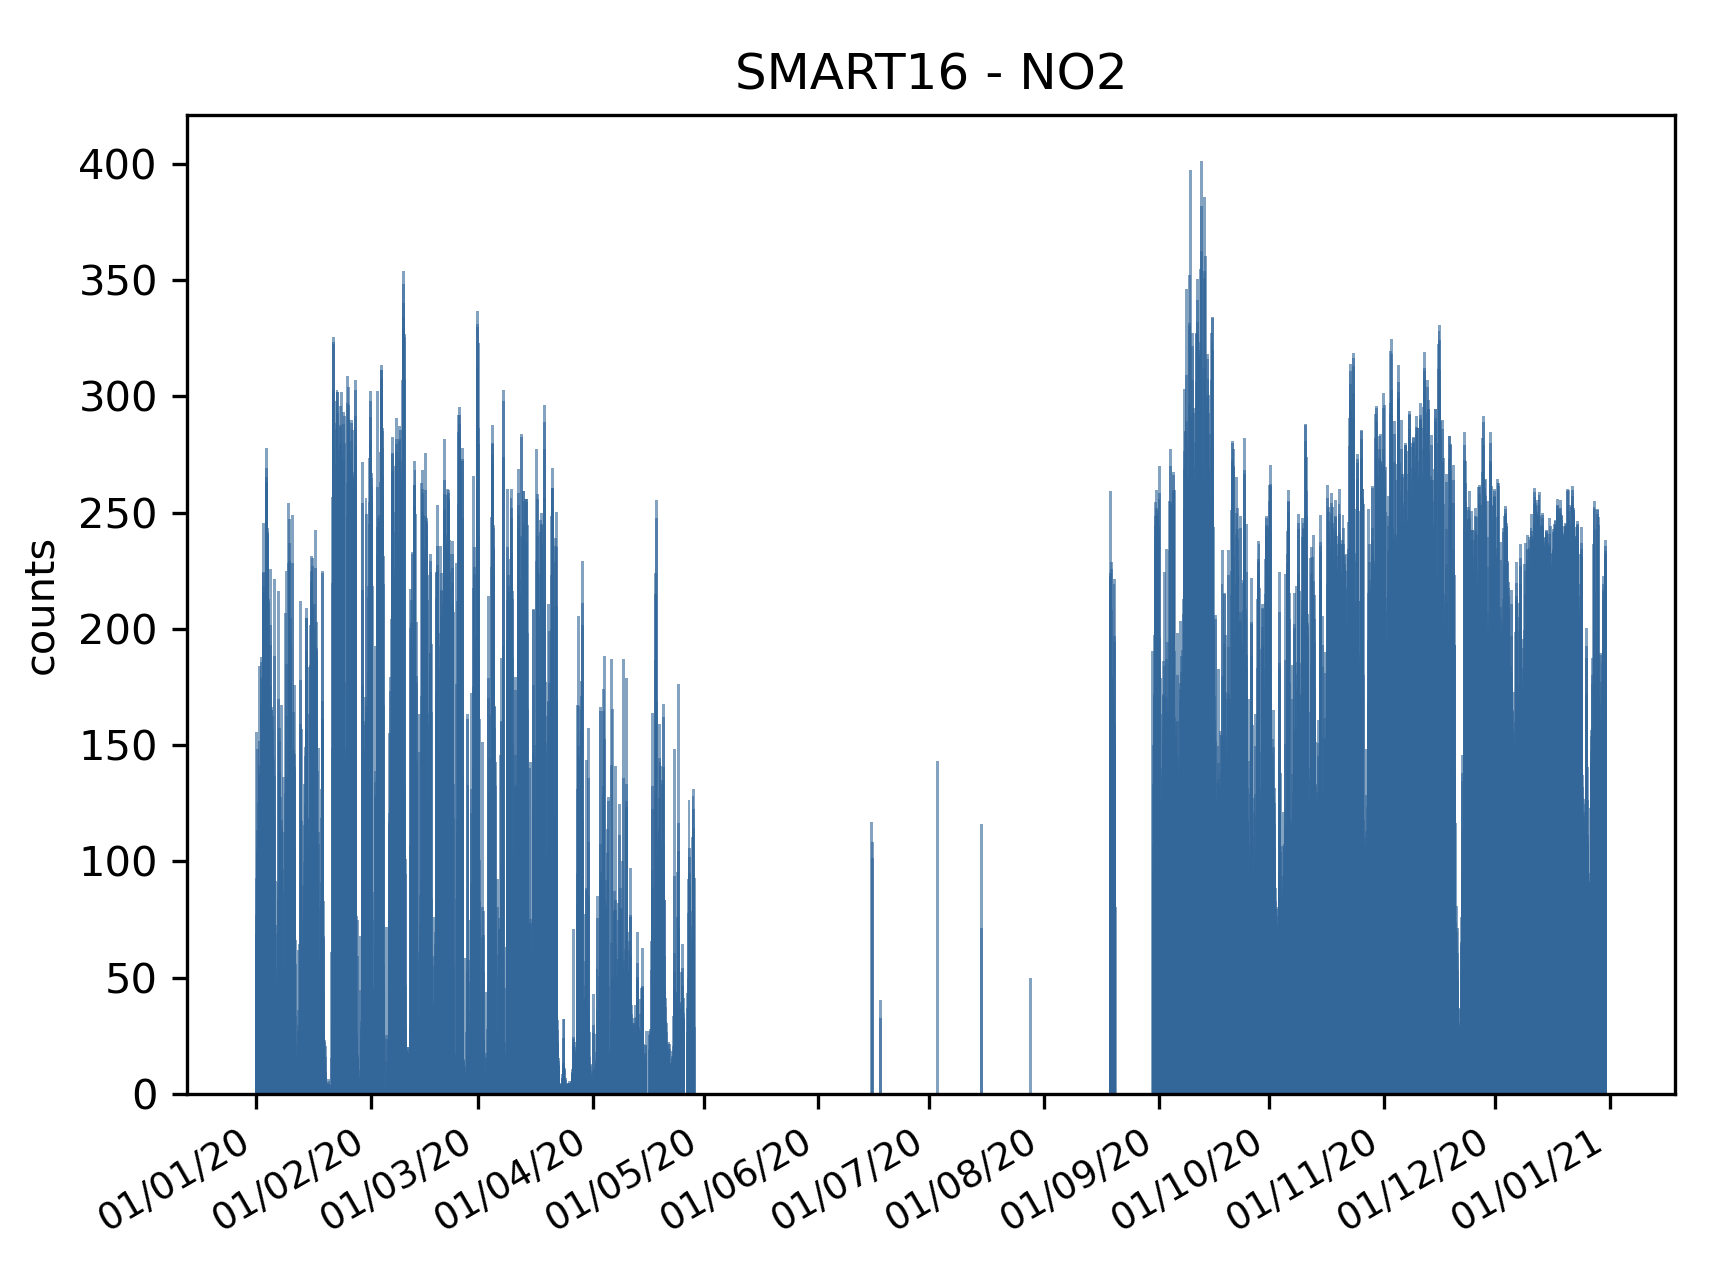
\includegraphics[width=7cm]{img/smart16_no2} }}%
    \caption{Frequenza di misurazione e andamento \ce{NO2} (SMART16)\\nel periodo 01/01/2020 - 31/12/2020}%
    \label{fig:smart16-no2}%
\end{figure}

\begin{figure}[H]
\centering
\captionsetup{justification=centering}
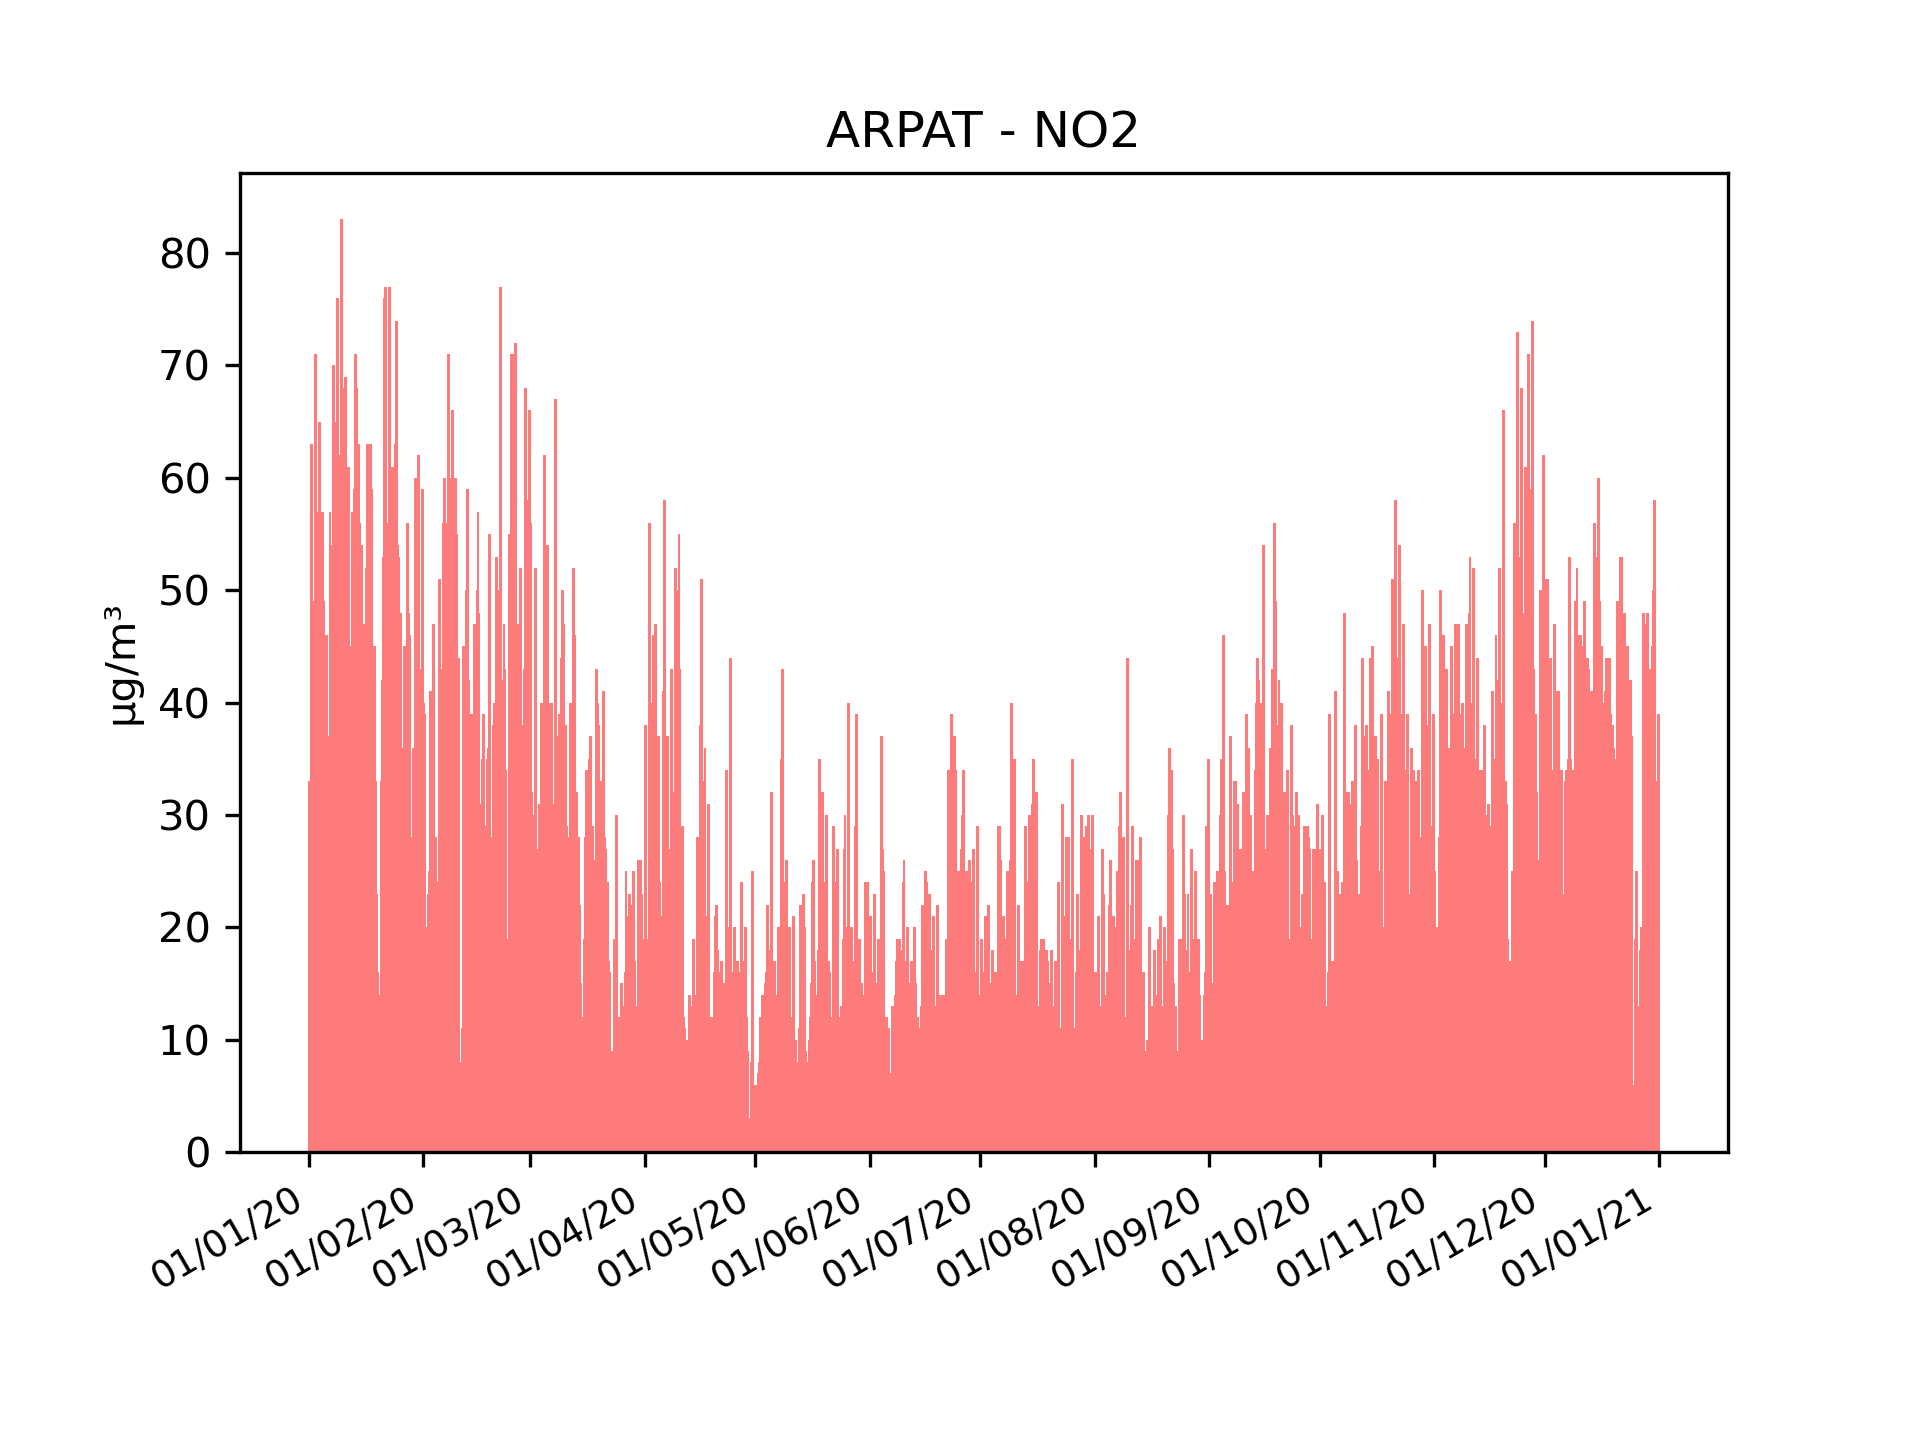
\includegraphics[width=0.85\textwidth,height=\textheight,keepaspectratio]{img/lu-capannori_no2_2020_cleaned_no2.png}
\caption{Andamento \ce{NO2} (in µg/m³) misurato dalla stazione ARPAT di Capannori nel periodo 01/01/2020 - 31/12/2020}
\label{fig:arpat-no2}
\end{figure}
\clearpage

\subsection{Dataset \ce{PM_{2.5}} e \ce{PM10}}\label{ssec:dataset-pm}
Il dataset di misurazioni \ce{PM_{2.5}} e \ce{PM10}, che mette a confronto i dati della centralina AirQino SMART16 e i dati di ARPAT (Capannori), risulta invece così strutturato:\\

\begin{table}[H]
\centering
\def\arraystretch{0.9}
\begin{tabular}{|l|l|l|l|}
\cline{2-4}
\multicolumn{1}{c|}{} & \textbf{Periodo} & \textbf{Unità} & \textbf{Frequenza dati} \\ \hline
\textbf{SMART16} & 01/09/2020 - 31/08/2021 & µg/m³ & ogni 1/2 minuti \\ \hline
\textbf{ARPAT} & 01/09/2020 - 31/08/2021 & µg/m³ & medie ogni 8h \\ \hline
\end{tabular}
\caption{Differenze tra i dati di SMART16 e ARPAT (per \ce{PM_{2.5}} e \ce{PM10})}
\label{tab:dataset-no2-tabella}
\end{table}

Il sensore utilizzato dalle centraline SMART è il \textbf{SDS011} (vedi \ref{ssec:hardware}) che ha la caratteristica di fornire l'uscita direttamente in unità ingegneristica (µg/m³), quindi in questo caso non c'è bisogno di convertire l'unità di misura nella fase di calibrazione (a differenza di quanto accade con \ce{NO2}).

Nella figura \ref{fig:arpat-pm-freq} è riportata la frequenza di misurazione (numero di misurazioni effettuate ogni ora) di \ce{PM_{2.5}} e \ce{PM10} nell'aria (in µg/m³) per la centralina SMART16 nel periodo di interesse (01/09/2020 - 31/08/2021).

\begin{figure}[H]
\centering
\captionsetup{justification=centering}
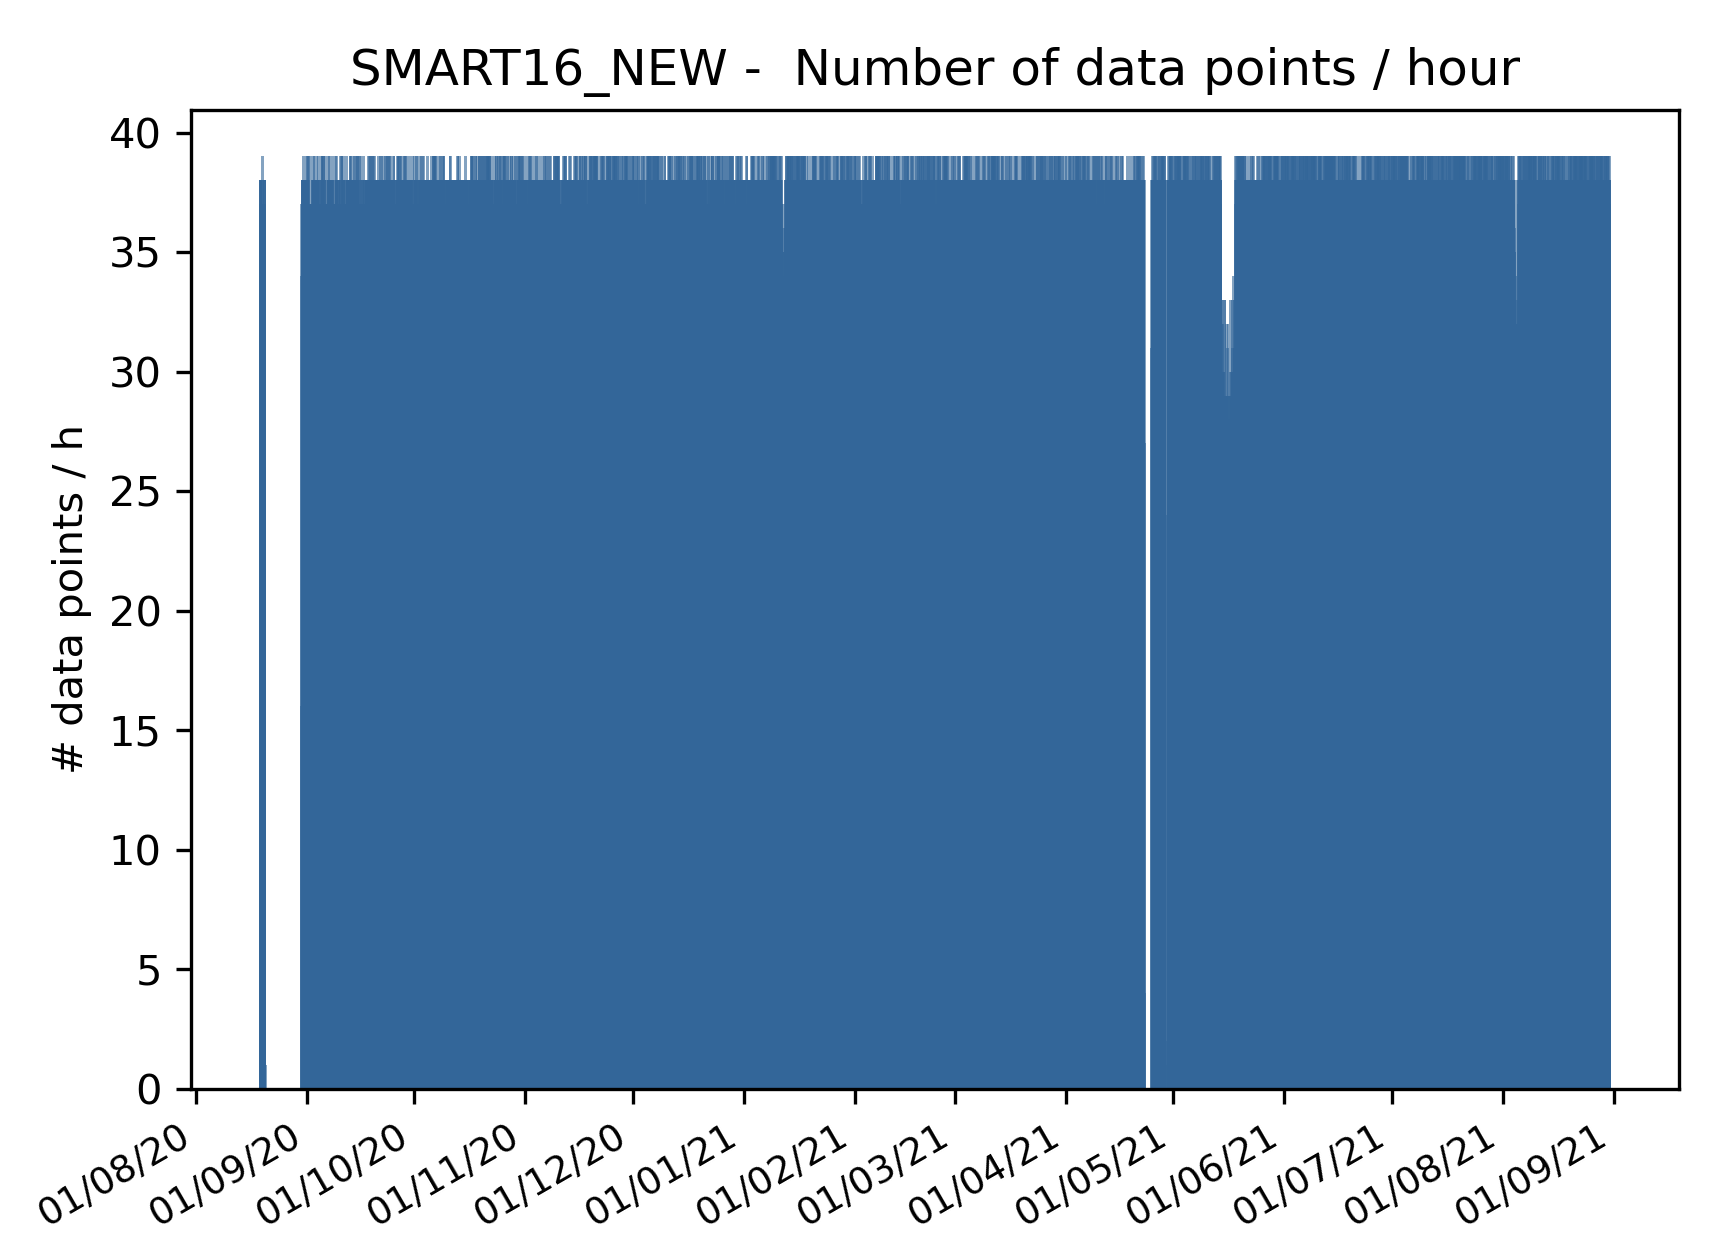
\includegraphics[width=0.58\textwidth,height=\textheight,keepaspectratio]{img/smart16_new_count.png}
\caption{Frequenza di misurazione \ce{PM_{2.5}} e \ce{PM10} (SMART16)}
\label{fig:arpat-pm-freq}
\end{figure}

Nella figura \ref{fig:smart16-pm} sono riportati gli andamenti della concentrazione di \ce{PM_{2.5}} e \ce{PM10} nell'aria (in µg/m³) per come sono state misurate dalla centralina SMART16 nel periodo di interesse (01/09/2020 - 31/08/2021).

La figura \ref{fig:arpat-pm} invece riporta gli andamenti della concentrazione di \ce{PM_{2.5}} e \ce{PM10} nell'aria (in µg/m³) misurato dalla stazione ARPAT di Capannori nello stesso periodo.

\begin{figure}[H]%
    \centering
    \captionsetup{justification=centering}
    \subfloat[\centering Andamento \ce{PM_{2.5}} (in µg/m³)]{{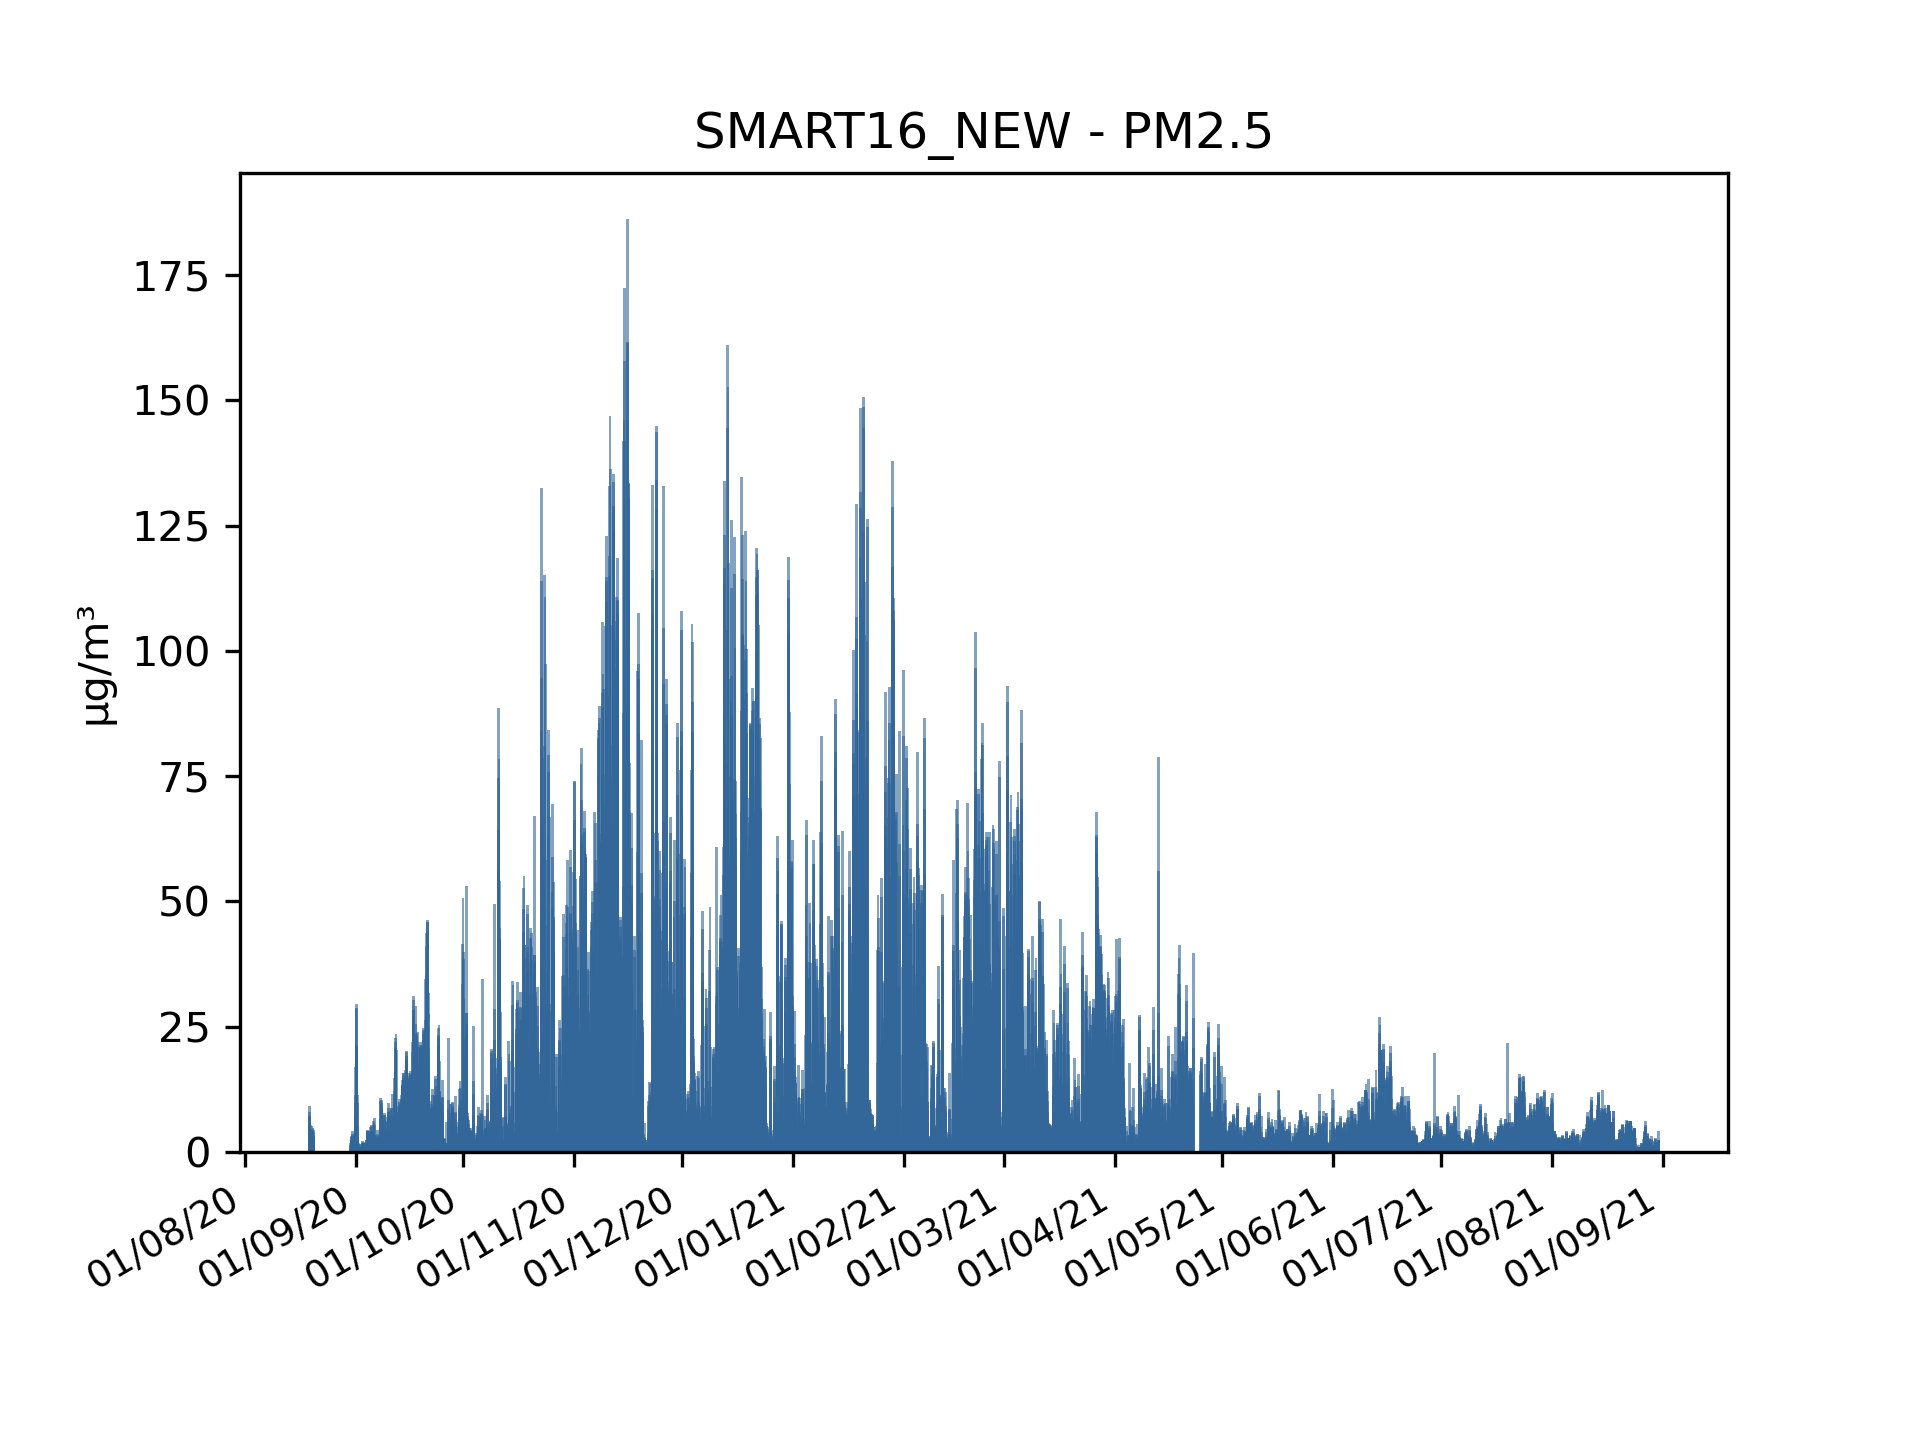
\includegraphics[width=6.7cm]{img/smart16_new_pm2.5} }}%
    \subfloat[\centering Andamento \ce{PM_{10}} (in µg/m³)]{{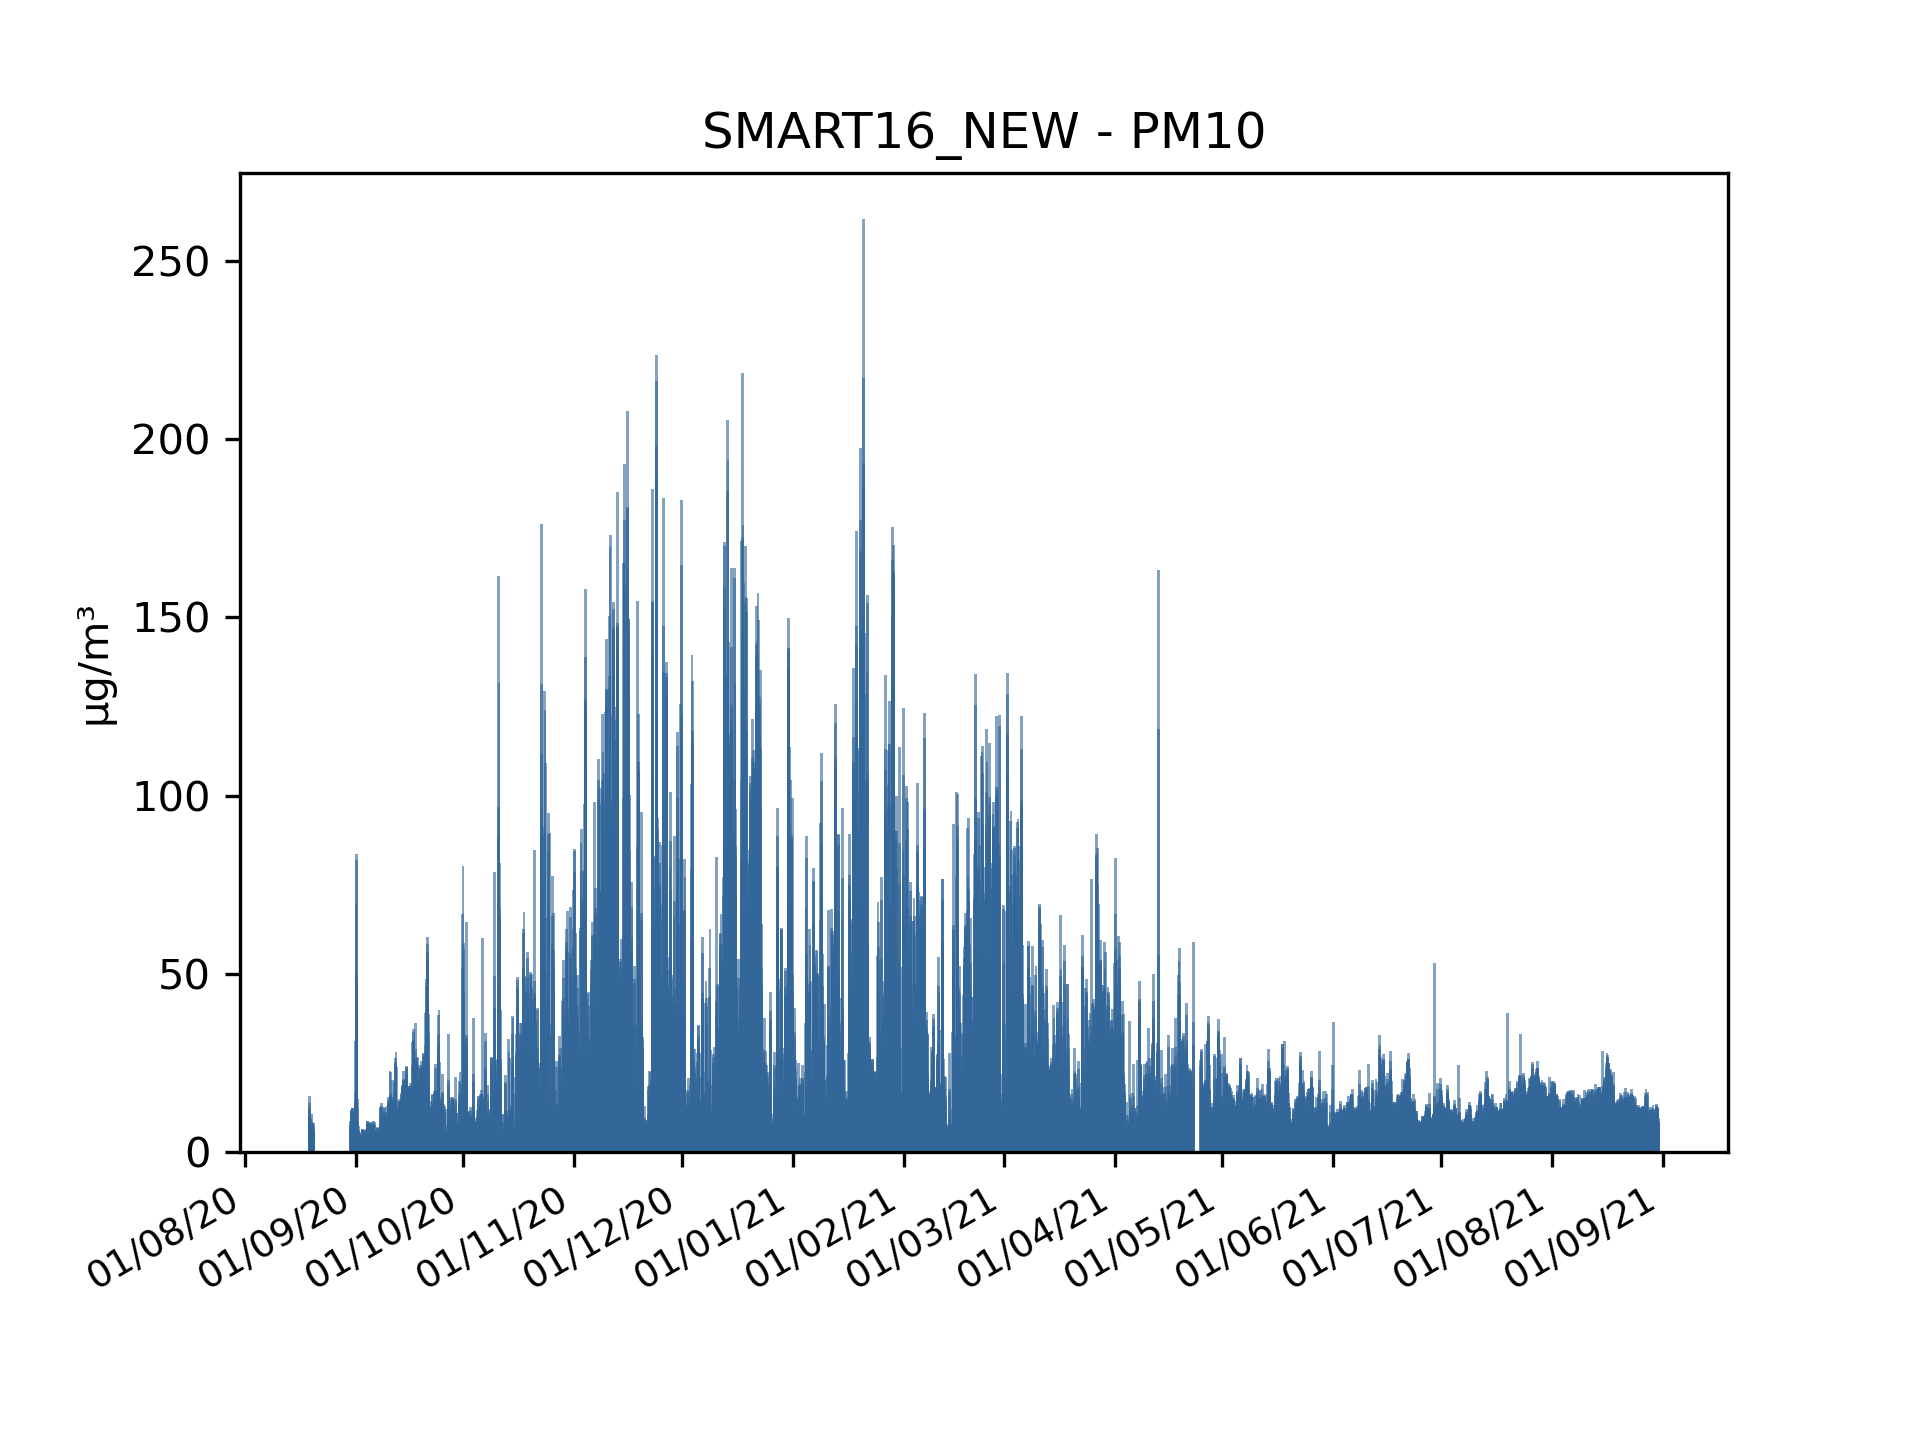
\includegraphics[width=6.7cm]{img/smart16_new_pm10} }}%
    \caption{Andamento \ce{PM_{2.5}} e \ce{PM10} (SMART16)\\nel periodo 01/09/2020 - 31/08/2021}%
    \label{fig:smart16-pm}%
\end{figure}

\begin{figure}[H]%
    \centering
    \captionsetup{justification=centering}
    \subfloat[\centering Andamento \ce{PM_{2.5}} (in µg/m³)]{{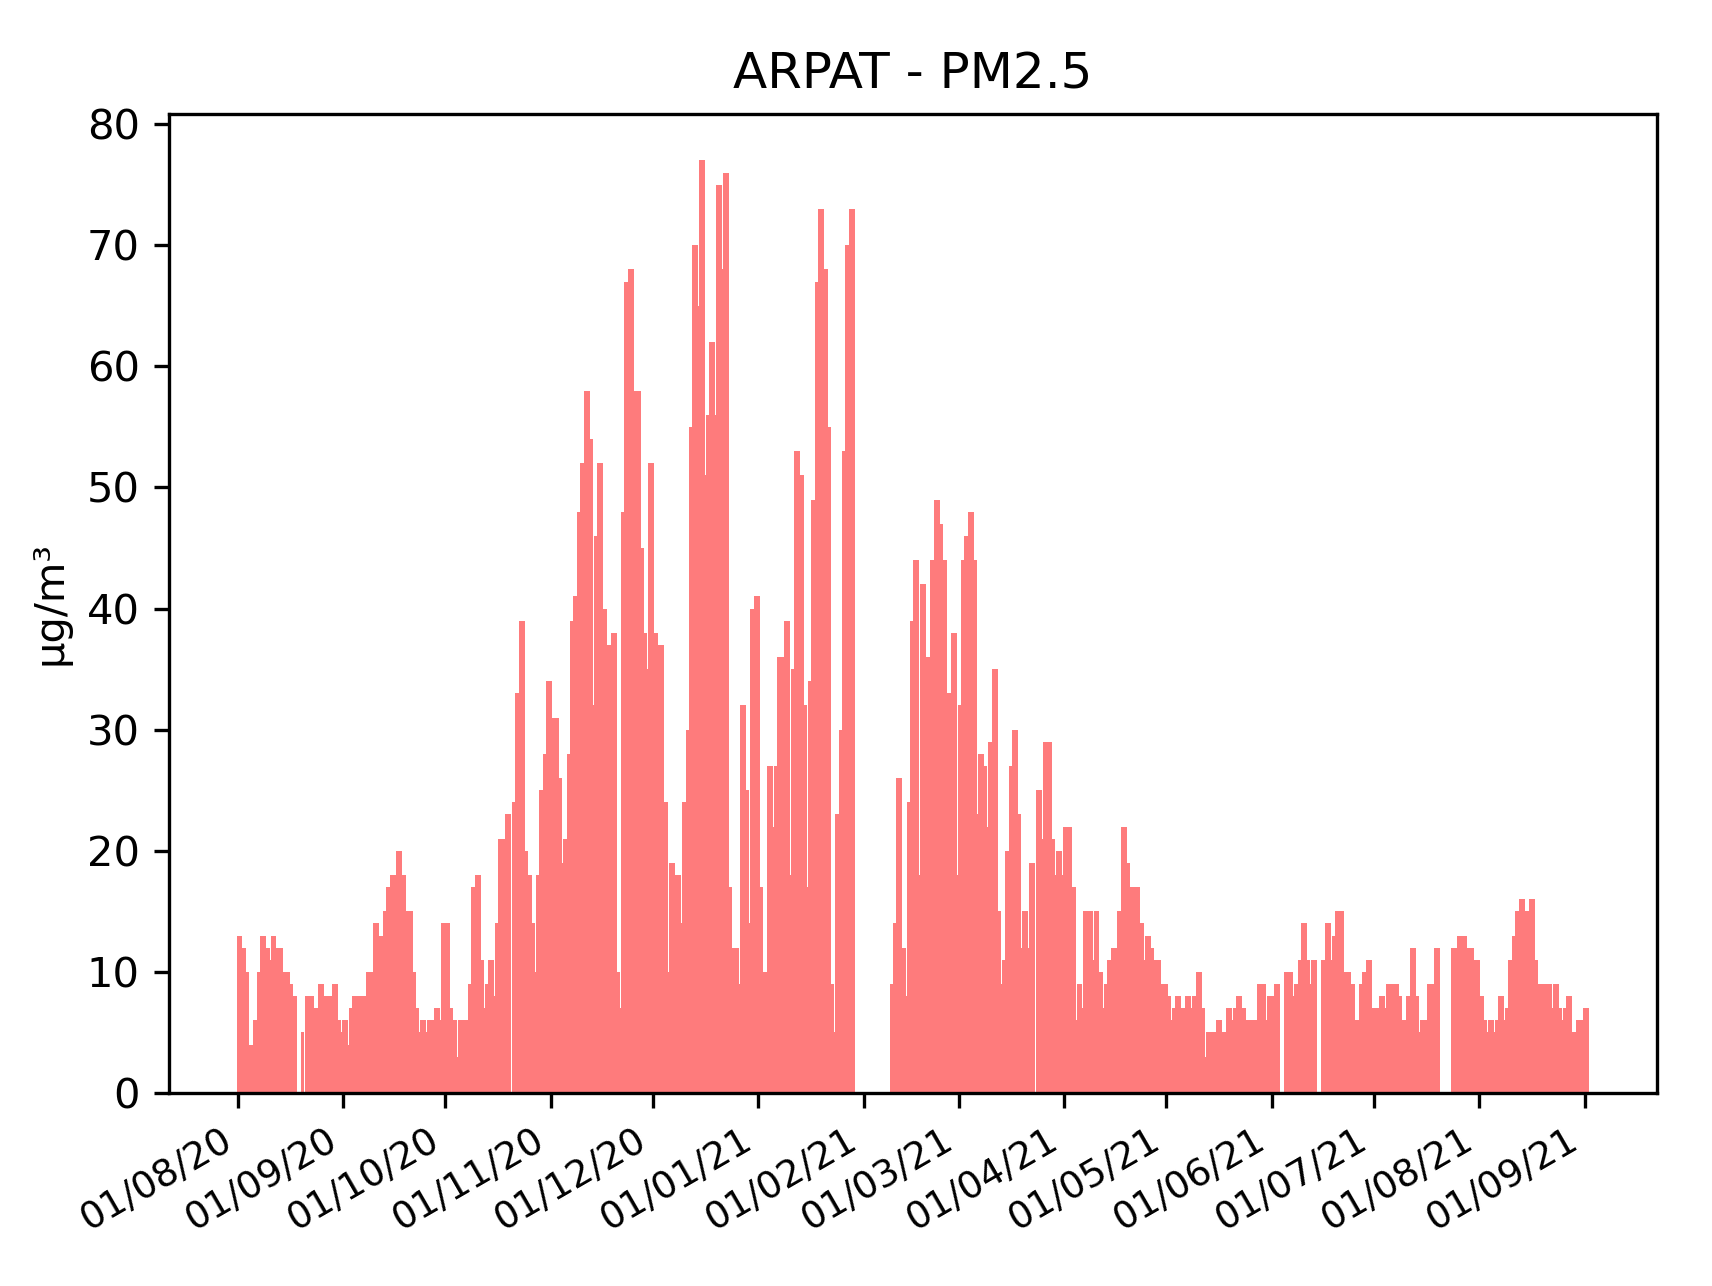
\includegraphics[width=6.7cm]{img/lu-capannori_pm_dati_orari_cleaned_pm2.5} }}%
    \subfloat[\centering Andamento \ce{PM_{10}} (in µg/m³)]{{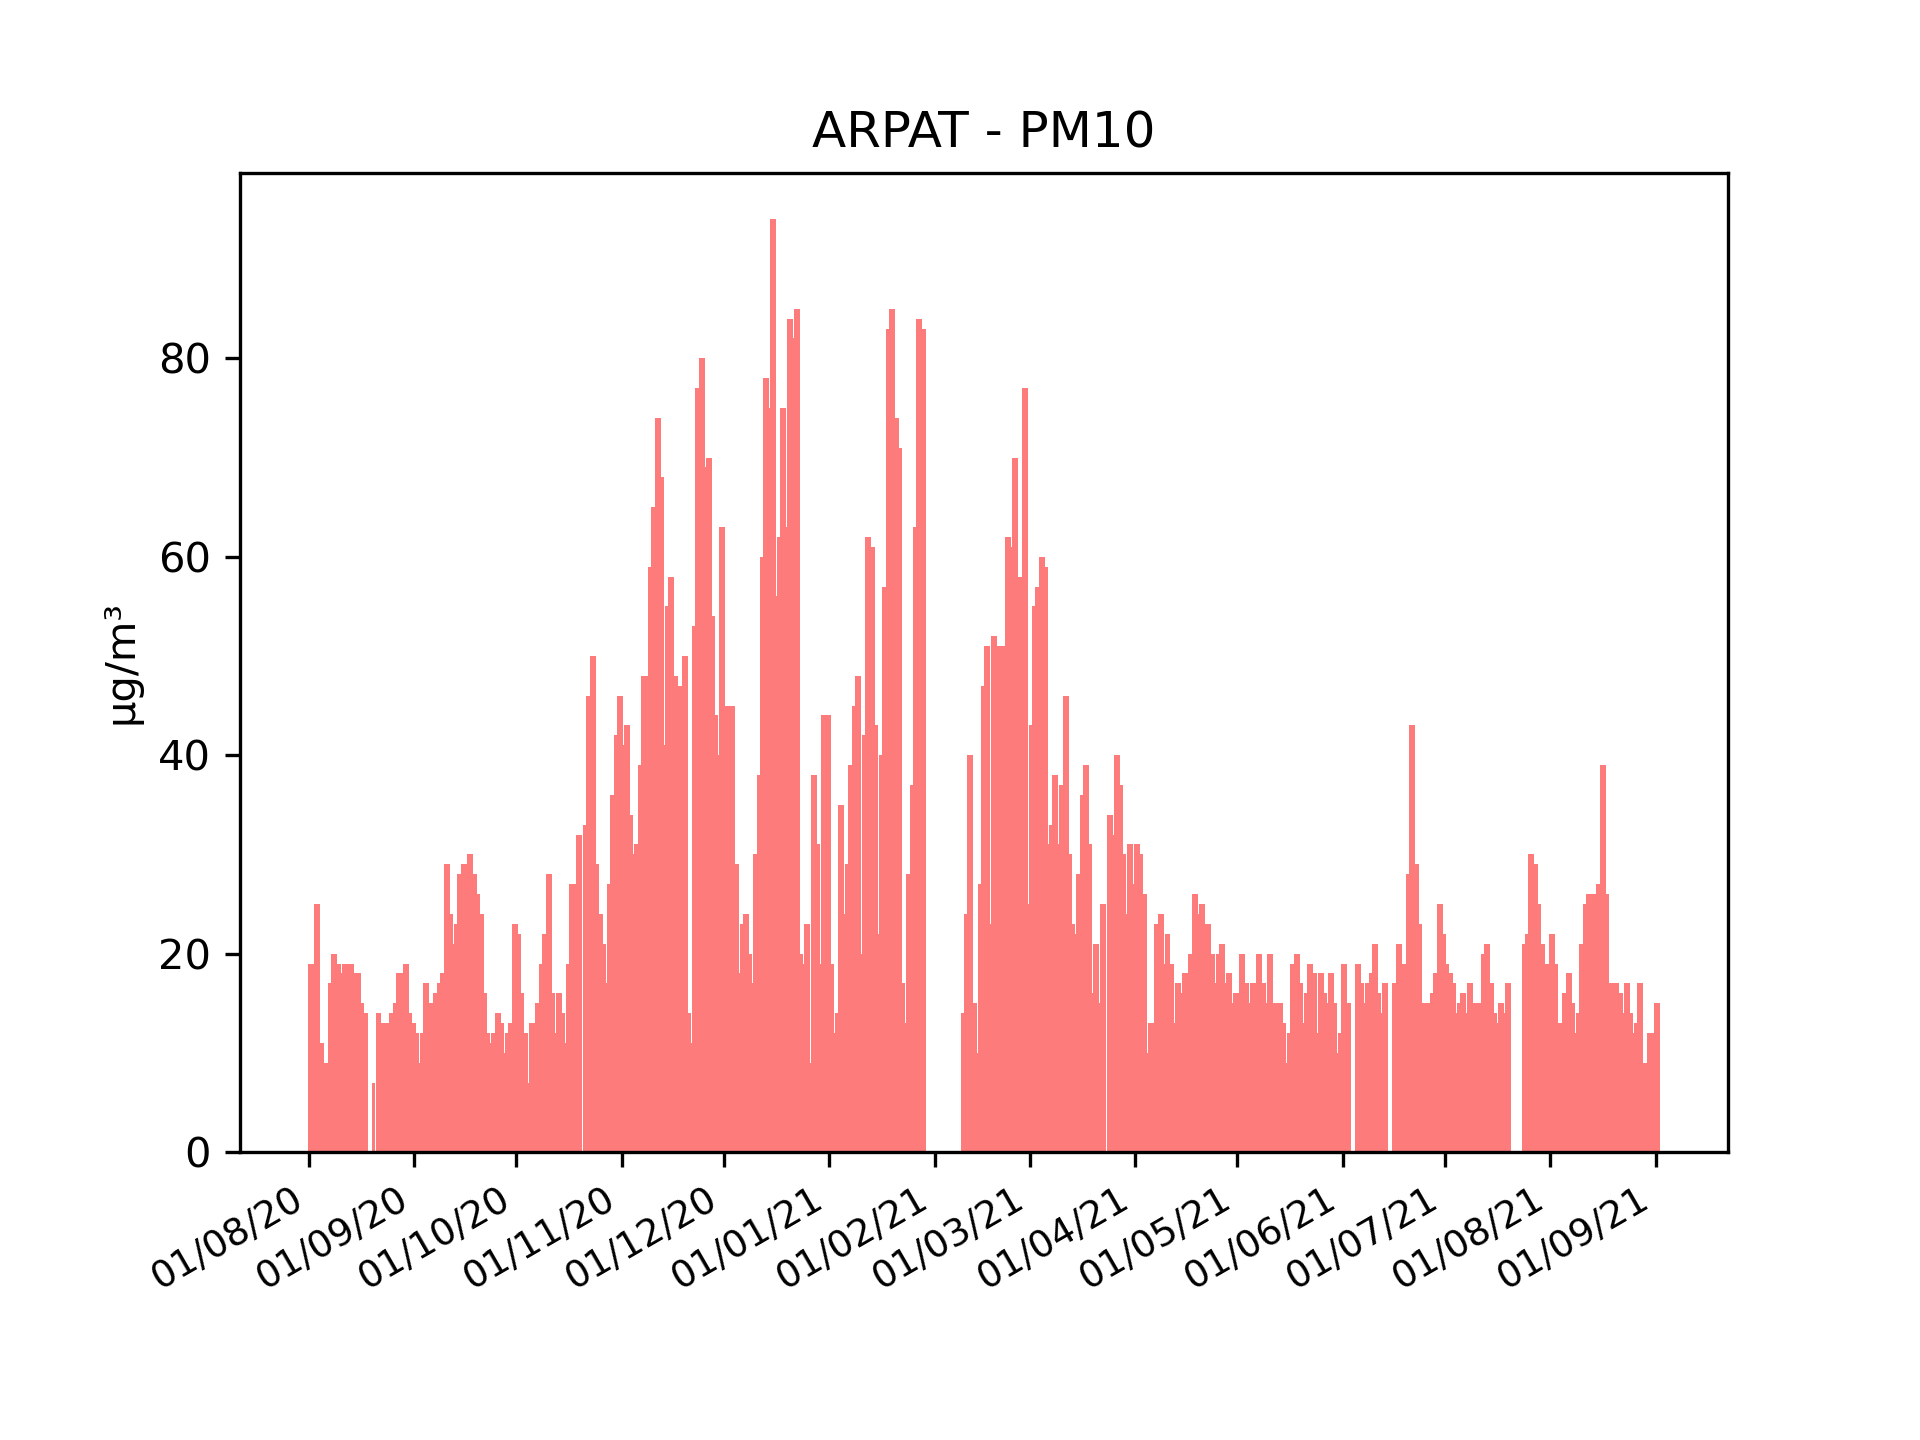
\includegraphics[width=6.7cm]{img/lu-capannori_pm_dati_orari_cleaned_pm10} }}%
    \caption{Andamento \ce{PM_{2.5}} e \ce{PM10} (ARPAT) nello stesso periodo}%
    \label{fig:arpat-pm}%
\end{figure}

\subsection{Preprocessamento}\label{ssec:preprocessamento}
Per facilitare il caricamento e l'elaborazione, si è resa necessaria una fase inziale di preprocessamento dei dati, descritta di seguito.

\subsubsection{Dataset ARPAT \ce{NO2}}
Il dataset originale \ce{NO2}, fornito da ARPAT, consiste in un file csv da 8785 righe, con encoding ISO-8859-1, valori separati da punto e virgola (;), e strutturato come in figura \ref{fig:ds-arpat}. In particolare:
\begin{itemize}
  \item La data è in formato AAAAMMGG (colonna 'DATA');
  \item L'ora risulta in formato intero (colonna 'ORA FINE MISURA', con valori da 1 a 24, dove 24 indica le 00:00);
  \item Data e ora sono da considerarsi con fuso orario locale;
  \item La colonna VALIDITÀ indica se la misurazione è valida oppure no;
  \item La media oraria è riportata in µg/m³.
\end{itemize}

\begin{figure}[H]
\centering
\captionsetup{justification=centering}
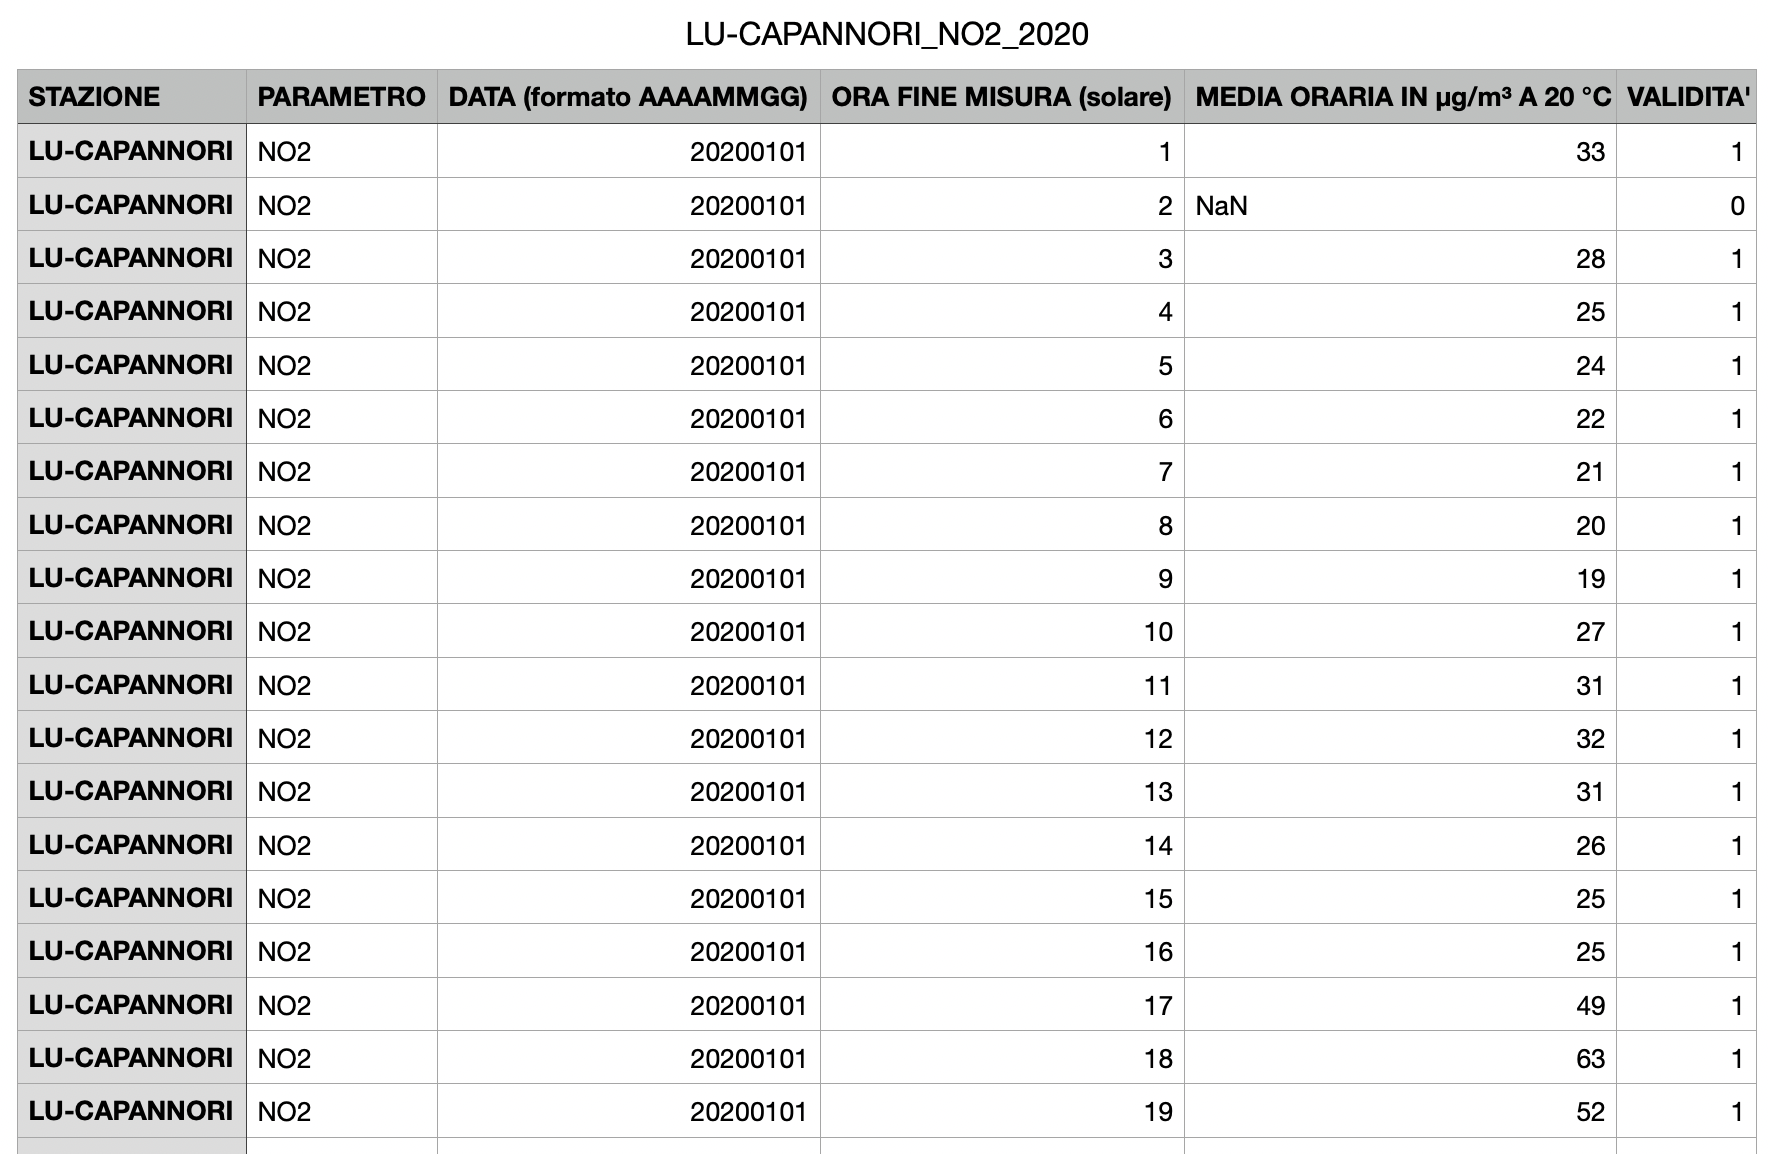
\includegraphics[width=0.75\textwidth,height=\textheight,keepaspectratio]{img/dataset_arpat_no2_prima.png}
\caption{Struttura del dataset originale \ce{NO2} fornito da ARPAT}
\label{fig:ds-arpat}
\end{figure}

In questa fase sono state effettuate le seguenti modifiche:
\begin{itemize}
  \item Data e ora sono state unite in una singola colonna;
  \item Data e ora sono state convertite in formato standard UTC\footnote{Il tempo coordinato universale o tempo civile, abbreviato con la sigla UTC, è il fuso orario scelto come riferimento globale, a partire dal quale sono calcolati tutti i fusi orari del mondo.} per conformarsi al dataset di AirQino;
  \item I dati non validi sono stati scartati;
  \item Le colonne sono state rinominate per semplicità ('data' per la data e 'avg' per il valore di \ce{NO2}).
\end{itemize}

Il risultato è un file csv di dimensioni ridotte che si presenta come riportato in figura \ref{fig:ds-arpat-dopo}:

\begin{figure}[H]
\centering
\captionsetup{justification=centering}
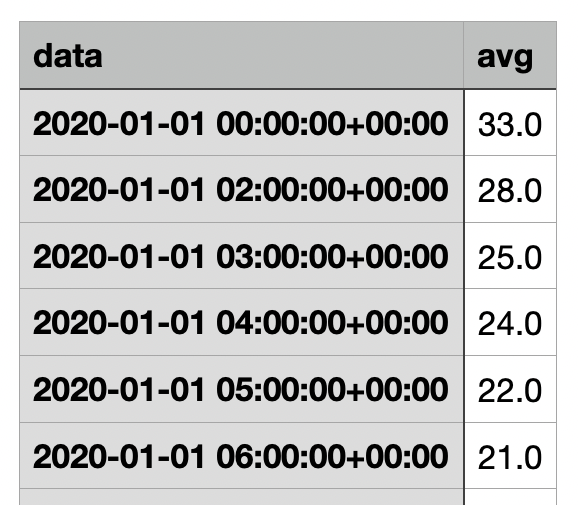
\includegraphics[width=0.60\textwidth,height=\textheight,keepaspectratio]{img/dataset_arpat_no2_dopo.png}
\caption{Struttura del dataset ARPAT \ce{NO2} processato}
\label{fig:ds-arpat-dopo}
\end{figure}

\subsubsection{Dataset ARPAT \ce{PM_{2.5}} e \ce{PM10}}
Il dataset originale \ce{PM_{2.5}} e \ce{PM10}, fornito da ARPAT, consiste in un singolo file csv da 33.674 righe con encoding UTF-8, valori separati da virgola (,), e strutturato come in figura \ref{fig:pm-arpat}. In particolare:
\begin{itemize}
  \item Ci sono dati dal 18/01/2018 al 20/11/2021, ma per questo lavoro è stato considerato solo il periodo 01/09/2020 - 31/08/2021;
  \item La data è in formato gg/mm/aaaa (colonna 'DATA');
  \item L'ora è in formato intero (colonna 'ORA' con valori da 1 a 24, dove 24 indica le 00:00);
  \item Data e ora sono da considerarsi con fuso orario locale;
  \item I valori di \ce{PM_{2.5}} e \ce{PM10} sono riportati rispettivamente nelle colonne 'PM2.5\_LU-CAPANNORI' e 'PM10\_LU-CAPANNORI';
  \item I dati sono riportati come medie orarie, ma di fatto rappresentano medie ogni 8 ore.
\end{itemize}

\begin{figure}[H]
\centering
\captionsetup{justification=centering}
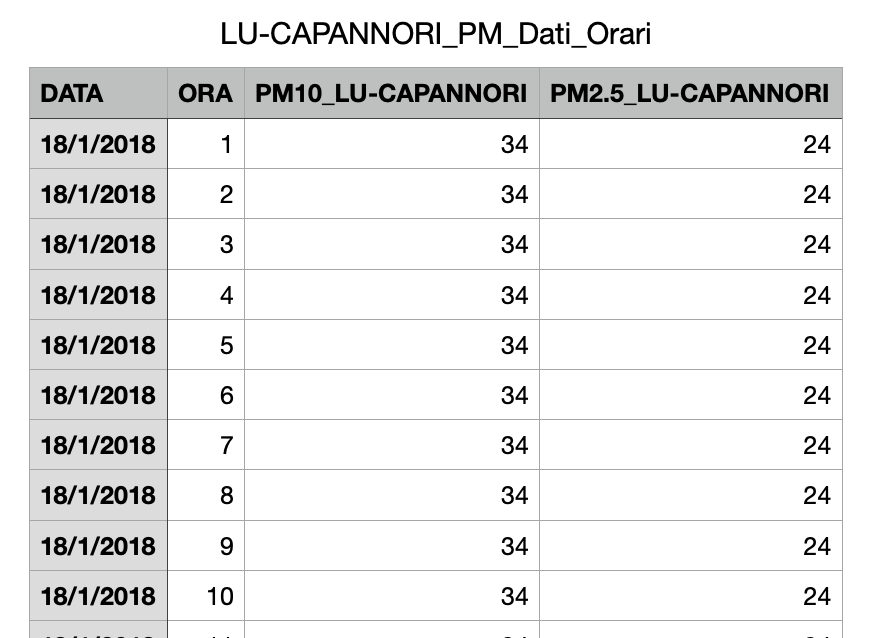
\includegraphics[width=0.7\textwidth,height=\textheight,keepaspectratio]{img/dataset_arpat_pm_prima.png}
\caption{Struttura del dataset originale ARPAT \ce{PM_{2.5}} e \ce{PM10}}
\label{fig:pm-arpat}
\end{figure}

Per questo dataset sono state effettuate le seguenti modifiche:
\begin{itemize}
  \item Data e ora sono state unite in una singola colonna;
  \item Data e ora sono state convertite in formato standard UTC per conformarsi al dataset di AirQino;
  \item I dati non validi sono stati scartati;
  \item Le colonne sono state rinominate per semplicità ('data' per la data, 'pm2.5' per i valori di \ce{PM_{2.5}} e 'pm10' per i valori di \ce{PM10});
  \item I dati sono stati ricampionati e salvati come medie ogni otto ore.\\
\end{itemize}

Il risultato è un file csv di 4211 righe e che si presenta come riportato in figura \ref{fig:ds-arpat-pm-dopo}:

\begin{figure}[H]
\centering
\captionsetup{justification=centering}
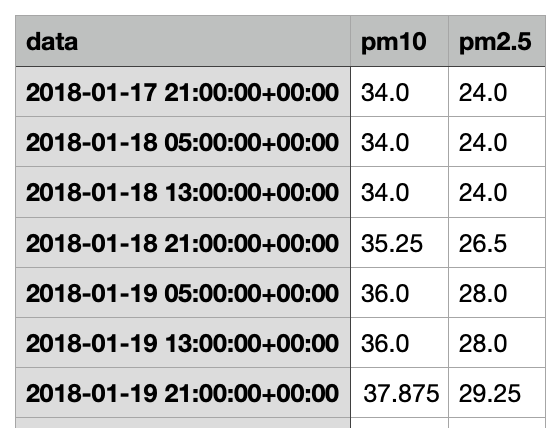
\includegraphics[width=0.65\textwidth,height=\textheight,keepaspectratio]{img/dataset_arpat_pm_dopo.png}
\caption{Struttura del dataset ARPAT \ce{PM_{2.5}} e \ce{PM10} processato\\con ricampionamento a 8 ore}
\label{fig:ds-arpat-pm-dopo}
\end{figure}


\subsubsection{Dataset SMART16}
Il dataset originale per la centralina SMART16 di AirQino consiste in due file csv (uno di 201.279 righe per \ce{NO2}, e l'altro di 324.431 righe per \ce{PM_{2.5}} e \ce{PM10}), strutturati rispettivamente come in figura \ref{fig:no2-smart-ds} e \ref{fig:pm-smart-ds}. In particolare:

\begin{itemize}
  \item Nel primo ci sono dati dal 01/01/2020 al 31/12/2020, nel secondo invece dal 18/08/2020 al 30/08/2021.
  \item Data e ora sono già in formato standard UTC;
  \item I valori di \ce{NO2} sono riportati nella colonna 'no2';
  \item I valori di \ce{PM_{2.5}} e \ce{PM10} sono riportati rispettivamente nelle colonne 'pm2\_5' e 'pm10';
  \item In entrambi i file sono riportate anche le coordinate inviate dalla centralina al momento della misurazione (colonne 'long' e 'lat');
  \item In entrambi i file i dati sono riportati con frequenza di 1/2 minuti.
\end{itemize}

\begin{figure}[H]
\centering
\captionsetup{justification=centering}
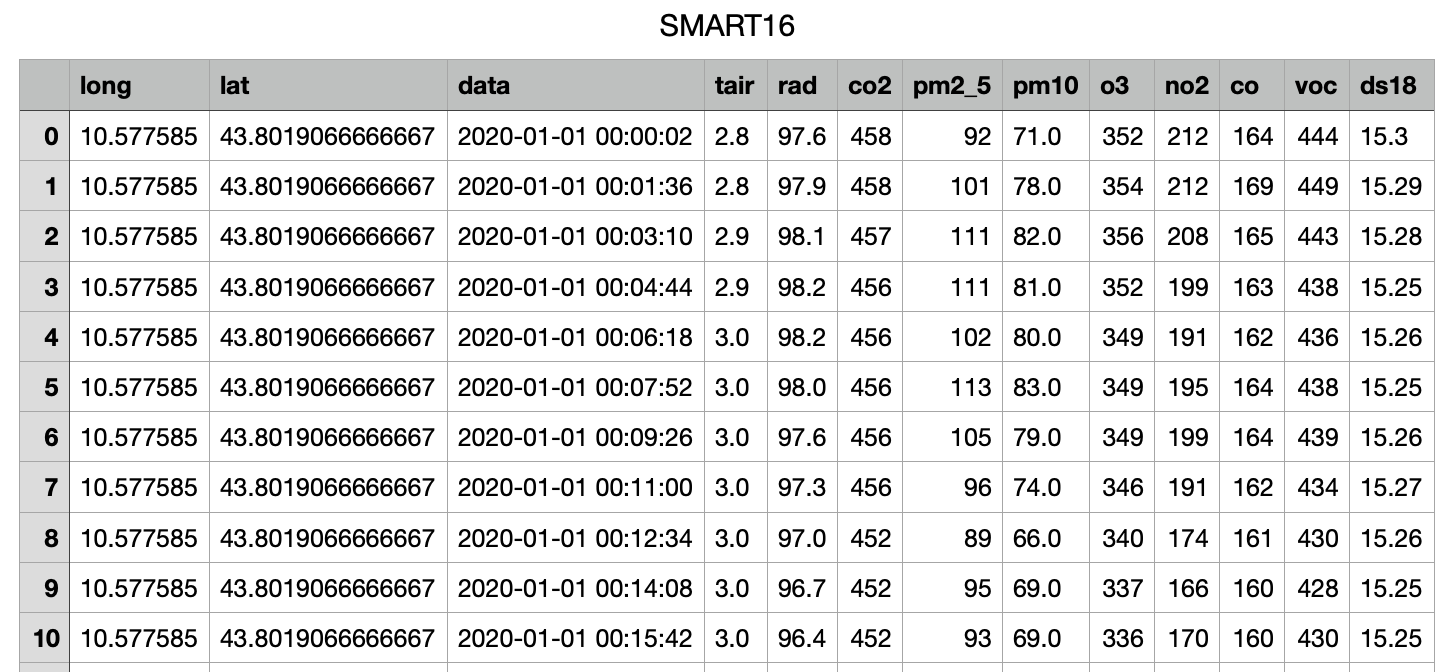
\includegraphics[width=0.7\textwidth,height=\textheight,keepaspectratio]{img/no2_smart_ds}
\caption{Struttura del dataset originale SMART16 per \ce{NO2}}
\label{fig:no2-smart-ds}
\end{figure}

\begin{figure}[H]
\centering
\captionsetup{justification=centering}
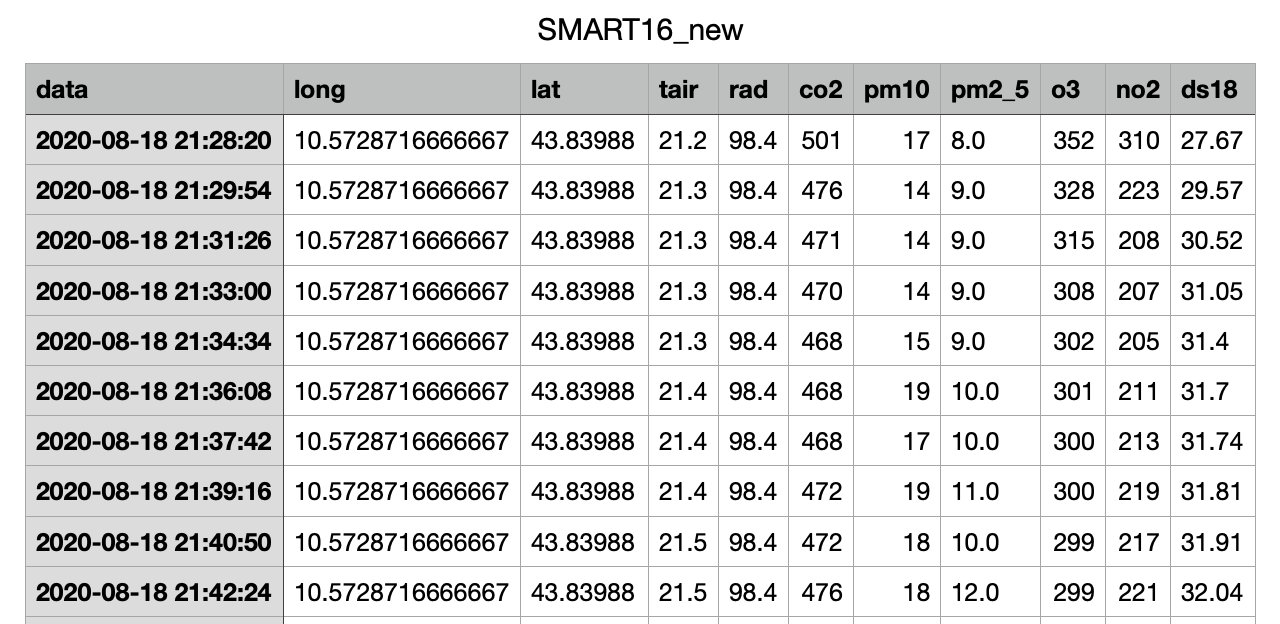
\includegraphics[width=0.7\textwidth,height=\textheight,keepaspectratio]{img/pm_smart_ds}
\caption{Struttura del dataset originale SMART16 per \ce{PM_{2.5}} e \ce{PM10}}
\label{fig:pm-smart-ds}
\end{figure}

Per questi due dataset sono state effettuate le seguenti modifiche:
\begin{itemize}
  \item I dati del dataset \ce{NO2} sono stati ricampionati a medie orarie;
  \item I dati del dataset \ce{PM_{2.5}} e \ce{PM10} sono stati ricampionati a otto ore;
  \item I dati non validi sono stati scartati.
\end{itemize}
Di seguito sono riportati i risultati del preprocessamento dei due dataset:

\begin{figure}[H]%
    \centering
    \captionsetup{justification=centering}
    \subfloat[\centering Dataset \ce{NO2} processato]{{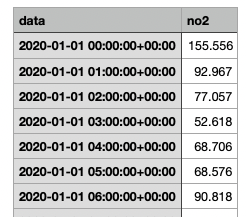
\includegraphics[width=6.7cm]{img/no2_smart_ds_dopo} }}%
    \subfloat[\centering Dataset \ce{PM_{2.5}} e \ce{PM10} processato]{{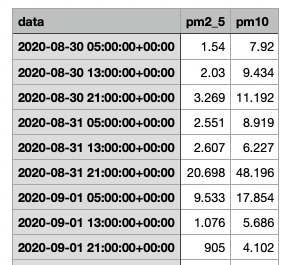
\includegraphics[width=6.4cm]{img/pm_smart_ds_dopo} }}%
    \caption{Struttura dei dataset SMART16 processati\\con ricampionamento a una e otto ore}%
    \label{fig:arpat-pm}%
\end{figure}

\subsubsection{Unione dei dataset}
In seguito, per facilitare l'elaborazione dei dati e l'applicazione delle tecniche di regressione (\ref{sec:regressione}), i dataset SMART e ARPAT (sia \ce{NO2} che \ce{PM_{2.5}} e \ce{PM10}) sono stati uniti in un unico dataset basandosi sul valore comune (colonna 'data').
I risultati di questa unione sono riportati di seguito (figure \ref{fig:no2-ds-final} e \ref{fig:pm-ds-final}) e rappresentano i dataset finali utilizzati nella fase di sperimentazione (\ref{sec:esperimenti}).

\begin{figure}[H]
\centering
\captionsetup{justification=centering}
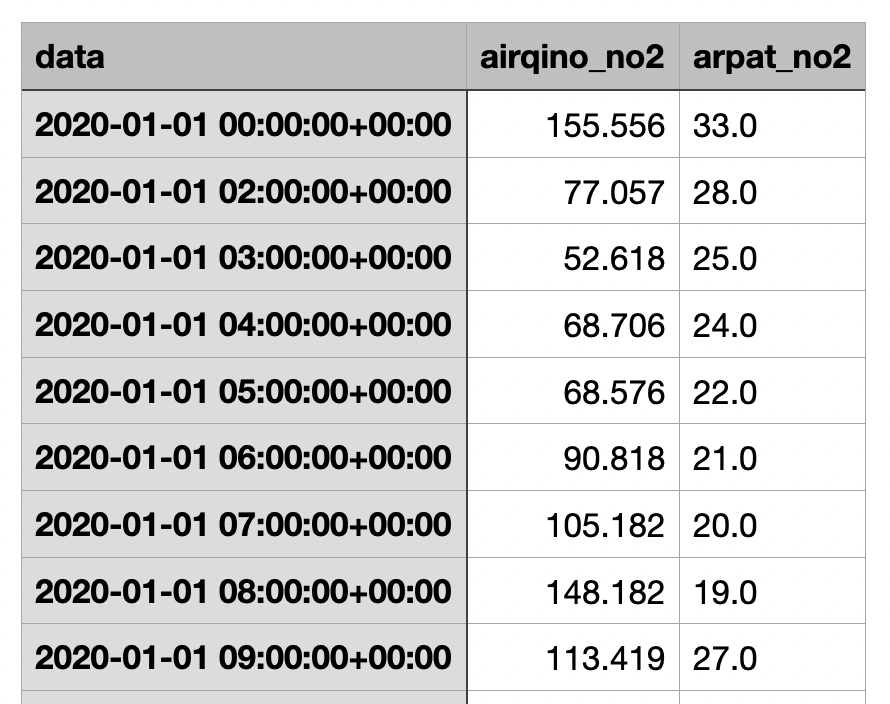
\includegraphics[width=0.55\textwidth,height=\textheight,keepaspectratio]{img/no2_ds_final}
\caption{Struttura del dataset finale per \ce{NO2} (SMART16 vs ARPAT)}
\label{fig:no2-ds-final}
\end{figure}

\begin{figure}[H]
\centering
\captionsetup{justification=centering}
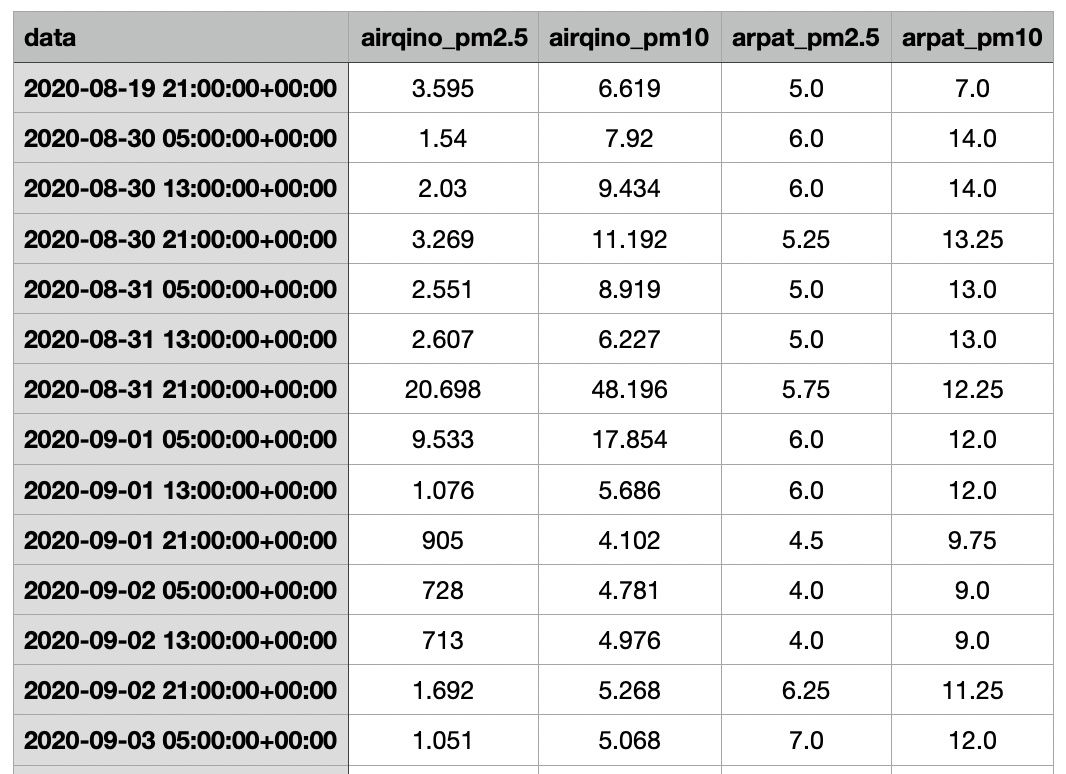
\includegraphics[width=0.55\textwidth,height=\textheight,keepaspectratio]{img/pm_ds_final}
\caption{Struttura del dataset finale per PM (SMART16 vs ARPAT)}
\label{fig:pm-ds-final}
\end{figure}

% Regressione
\section{Regressione}\label{sec:regressione}
Nella statistica applicata si osserva (o si ipotizza) l’esistenza di relazioni fra due o più grandezze. Sorge allora il problema di determinare una funzione che, in base ai dati ricavati mediante esperimenti o rilevazioni statistiche, rappresenti questi relazioni permettendo di analizzare meglio i fenomeni osservati. 

Con il termine regressione si intende proprio una tecnica statistica che serve a stimare la relazione esistente tra due o più variabili.

\subsection{Introduzione}\label{ssec:regressione-introduzione}
Limitando lo studio a problemi che stabiliscono relazioni fra due sole variabili, si tratta, partendo dalle coppie $(x_i, y_i)$ di dati rilevati, di determinare una funzione $y=f(x)$ che rappresenti la relazione.

Per fare questo si può procedere in due modi:

\begin{itemize}
  \item determinare una funzione che assuma esattamente i valori $(x_i, y_i)$ rilevati;
  \item determinare una funzione che si accosti il più possibile ai punti $(x_i, y_i)$.
\end{itemize}

La prima opzione, ovvero la ricerca di una funzione (generalmente espressa da un polinomio) che passi esattamente per i punti $(x_i, y_i)$ è piuttosto laboriosa. Nelle applicazioni statistiche si preferisce invece determinare la funzione il cui grafico si avvicini il più possibile ai punti rilevati.

Osservando l’andamento del fenomeno si sceglie il tipo di funzione interpolatrice: lineare, quadratica, esponenziale, ecc. e quindi si procede alla determinazione dei parametri, ossia delle costanti che compaiono nella funzione scelta in modo che sia soddisfatta una condizione di accostamento prefissata.

Per conseguire questo scopo il metodo più utilizzato è il metodo dei \textbf{minimi quadrati}, che costituisce un’applicazione della ricerca del minimo di una funzione di più variabili mediante gli strumenti dell’analisi infinitesimale.

Considerate due variabili $X$ e $Y$ sulle quali vengono effettuate $n$ rilevazioni: $$\left(x_{1}, y_{1}\right),\left(x_{2}, y_{2}\right), \ldots,\left(x_{i}, y_{i}\right), \ldots,\left(x_{n}, y_{n}\right)$$

Sia $y=f(x; a, b, c, ..., k)$ la funzione interpolatrice scelta. Siano inoltre $\hat{y}_{i}$ valori predetti sulla curva corrispondenti ai valori $x_i$ rilevati.

La condizione di accostamento data dal metodo dei minimi quadrati è quella di determinare i valori dei parametri in modo che sia minima la somma dei quadrati delle differenze fra i valori osservati $y_i$ e i valori predetti $\hat{y}_i$ (figura \ref{fig:minimi_quadrati}), ovvero:

$$\varphi(a, b, c, \ldots, k)=\sum_{i=1}^{n}\left[y_{i}-f\left(x_{i} ; a, b, c, \ldots, k\right)\right]^{2}$$\smallskip

dove i valori $x_i$ e $y_i$ sono noti, mentre sono incogniti i parametri $a , b , c , … , k$ della funzione. \cite{excel_per_statistica_belluco}

\begin{figure}[H]
\centering
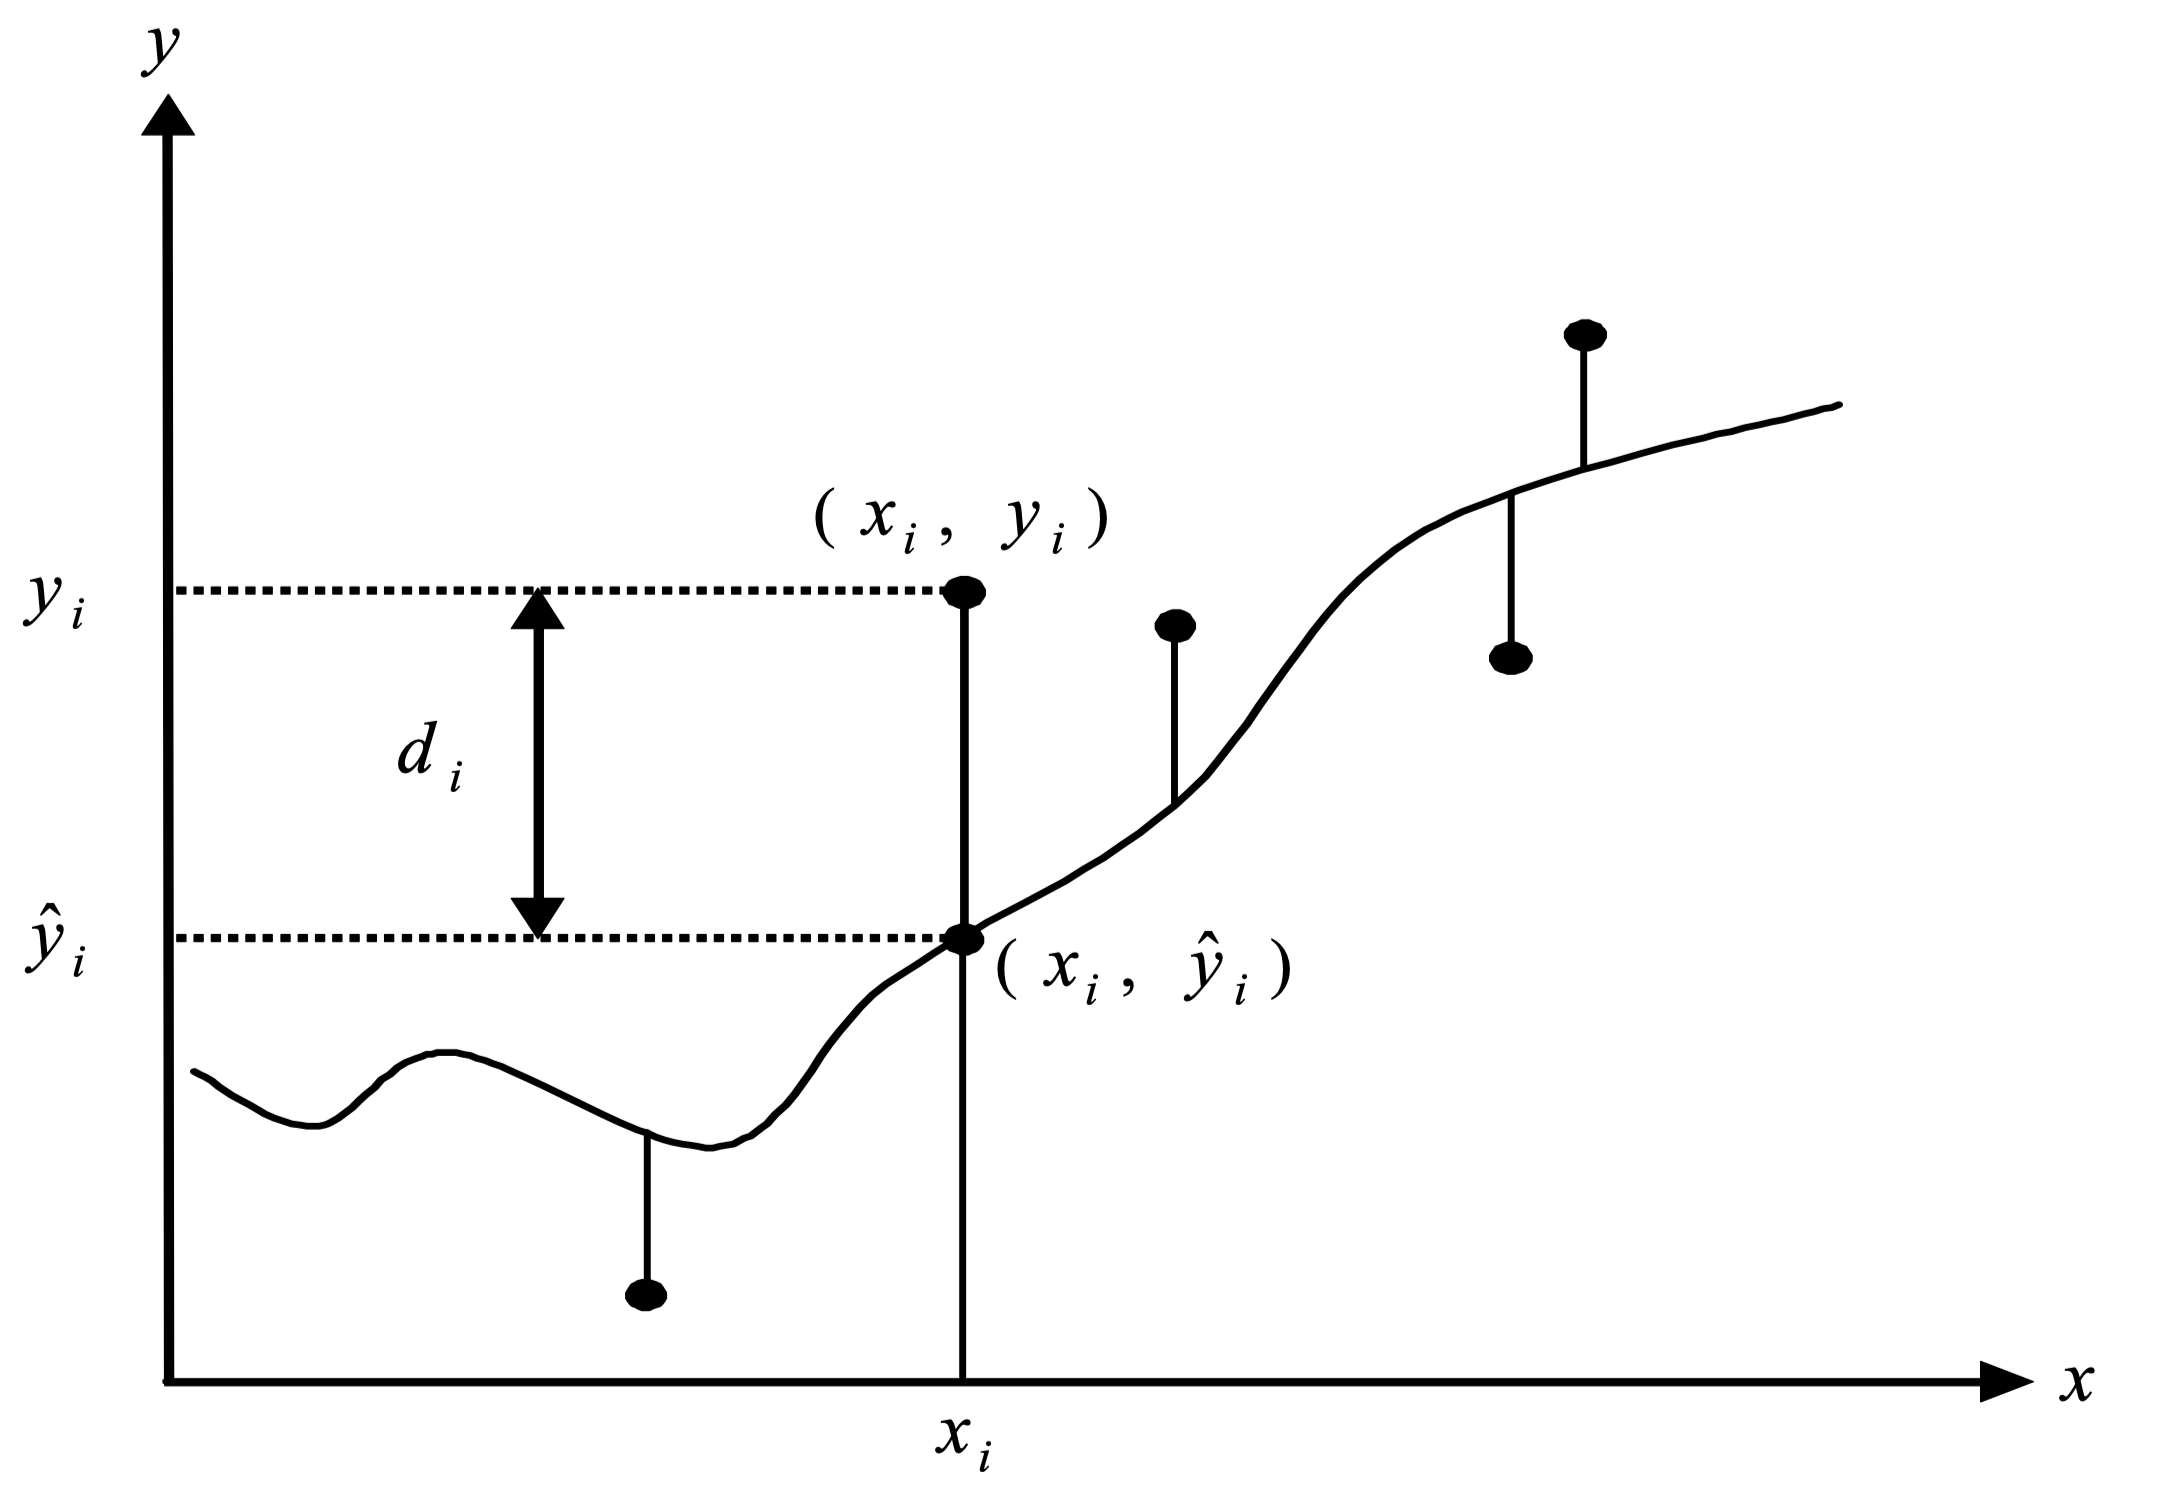
\includegraphics[width=0.75\textwidth,height=\textheight,keepaspectratio]{img/minimi_quadrati.png}
\caption{Condizione dei \textit{minimi quadrati} \cite{excel_per_statistica_belluco}}
\label{fig:minimi_quadrati}
\end{figure}

\subsection{Correlazione e coefficiente di determinazione}\label{ssec:regressione-correlazione}

Quando la dipendenza tra le due variabili è lineare, si parla di correlazione lineare, e può essere valutata mediante il coefficiente di correlazione lineare ($r$):

$$r=\frac{\sum_{i=1}^{n}\left(x_{i}-\bar{x}\right)\left(y_{i}-\bar{y}\right)}{\sqrt{\sum_{i=1}^{n}\left(x_{i}-\bar{x}\right)^{2}} \sqrt{\sum_{i=1}^{n}\left(y_{i}-\bar{y}\right)^{2}}}$$\smallskip

dove il termine al numeratore rappresenta la \textit{covarianza} di $X$ e $Y$, cioè la variabilità congiunta delle coppie ($x_i$, $y_i$) di valori corrispondenti rispetto al proprio valor medio; il denominatore invece rappresenta il prodotto delle deviazioni standard di $X$ ed $Y$.

Il coefficiente di correlazione lineare gode di importanti proprietà:

\begin{itemize}
  \item $-1 \le r \le 1$;
  \item si ha $r=1$ quando tutti i dati sono allineati lungo una retta crescente (figura \ref{fig:positive_correlation});
    \begin{figure}[H]
\centering
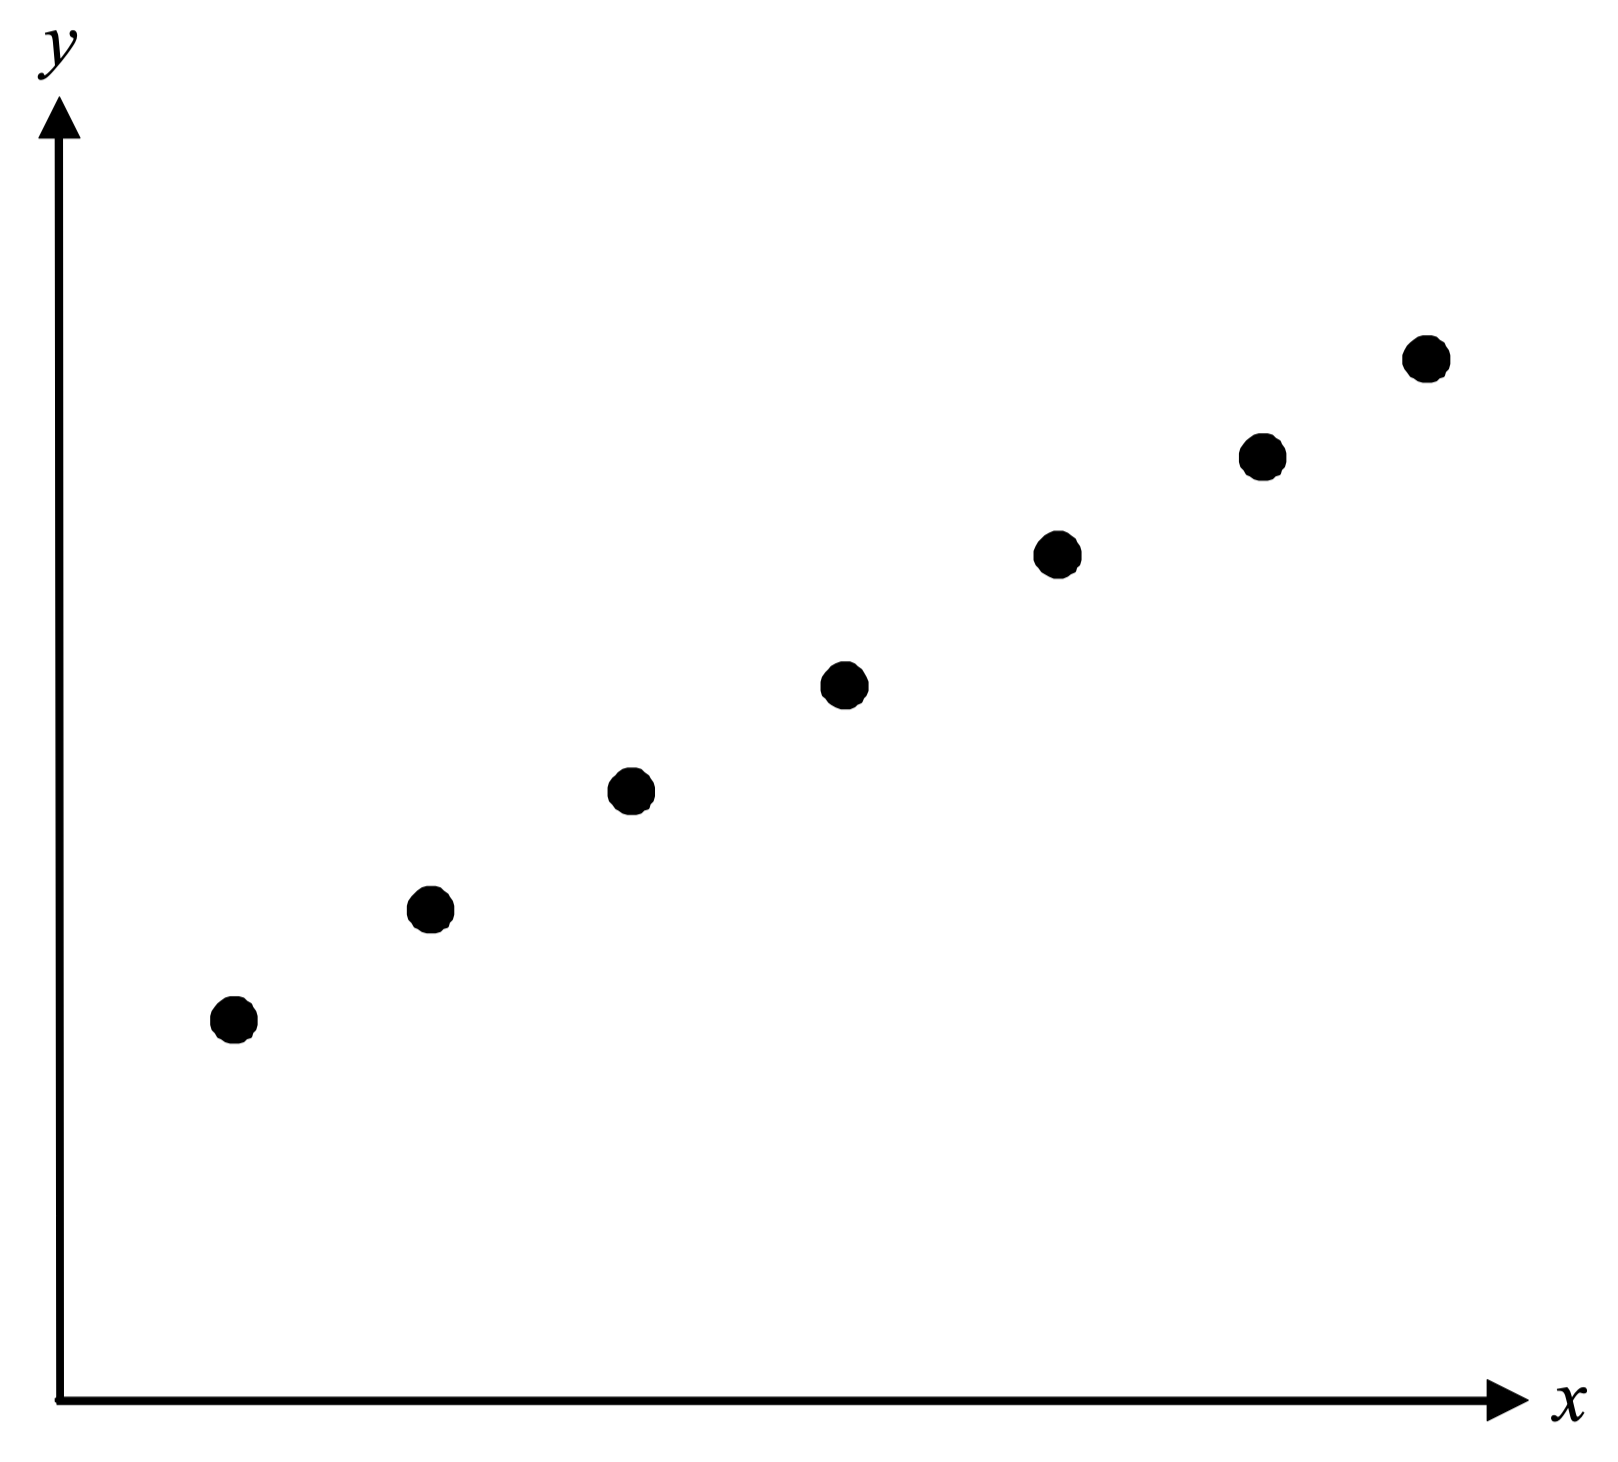
\includegraphics[width=0.45\textwidth,height=\textheight,keepaspectratio]{img/positive_correlation.png}
\caption{Correlazione lineare positiva}
\label{fig:positive_correlation}
\end{figure}

  \item si ha $r=-1$ quando tutti i dati sono allineati lungo una retta decrescente  (figura \ref{fig:negative_correlation});
      \begin{figure}[H]
\centering
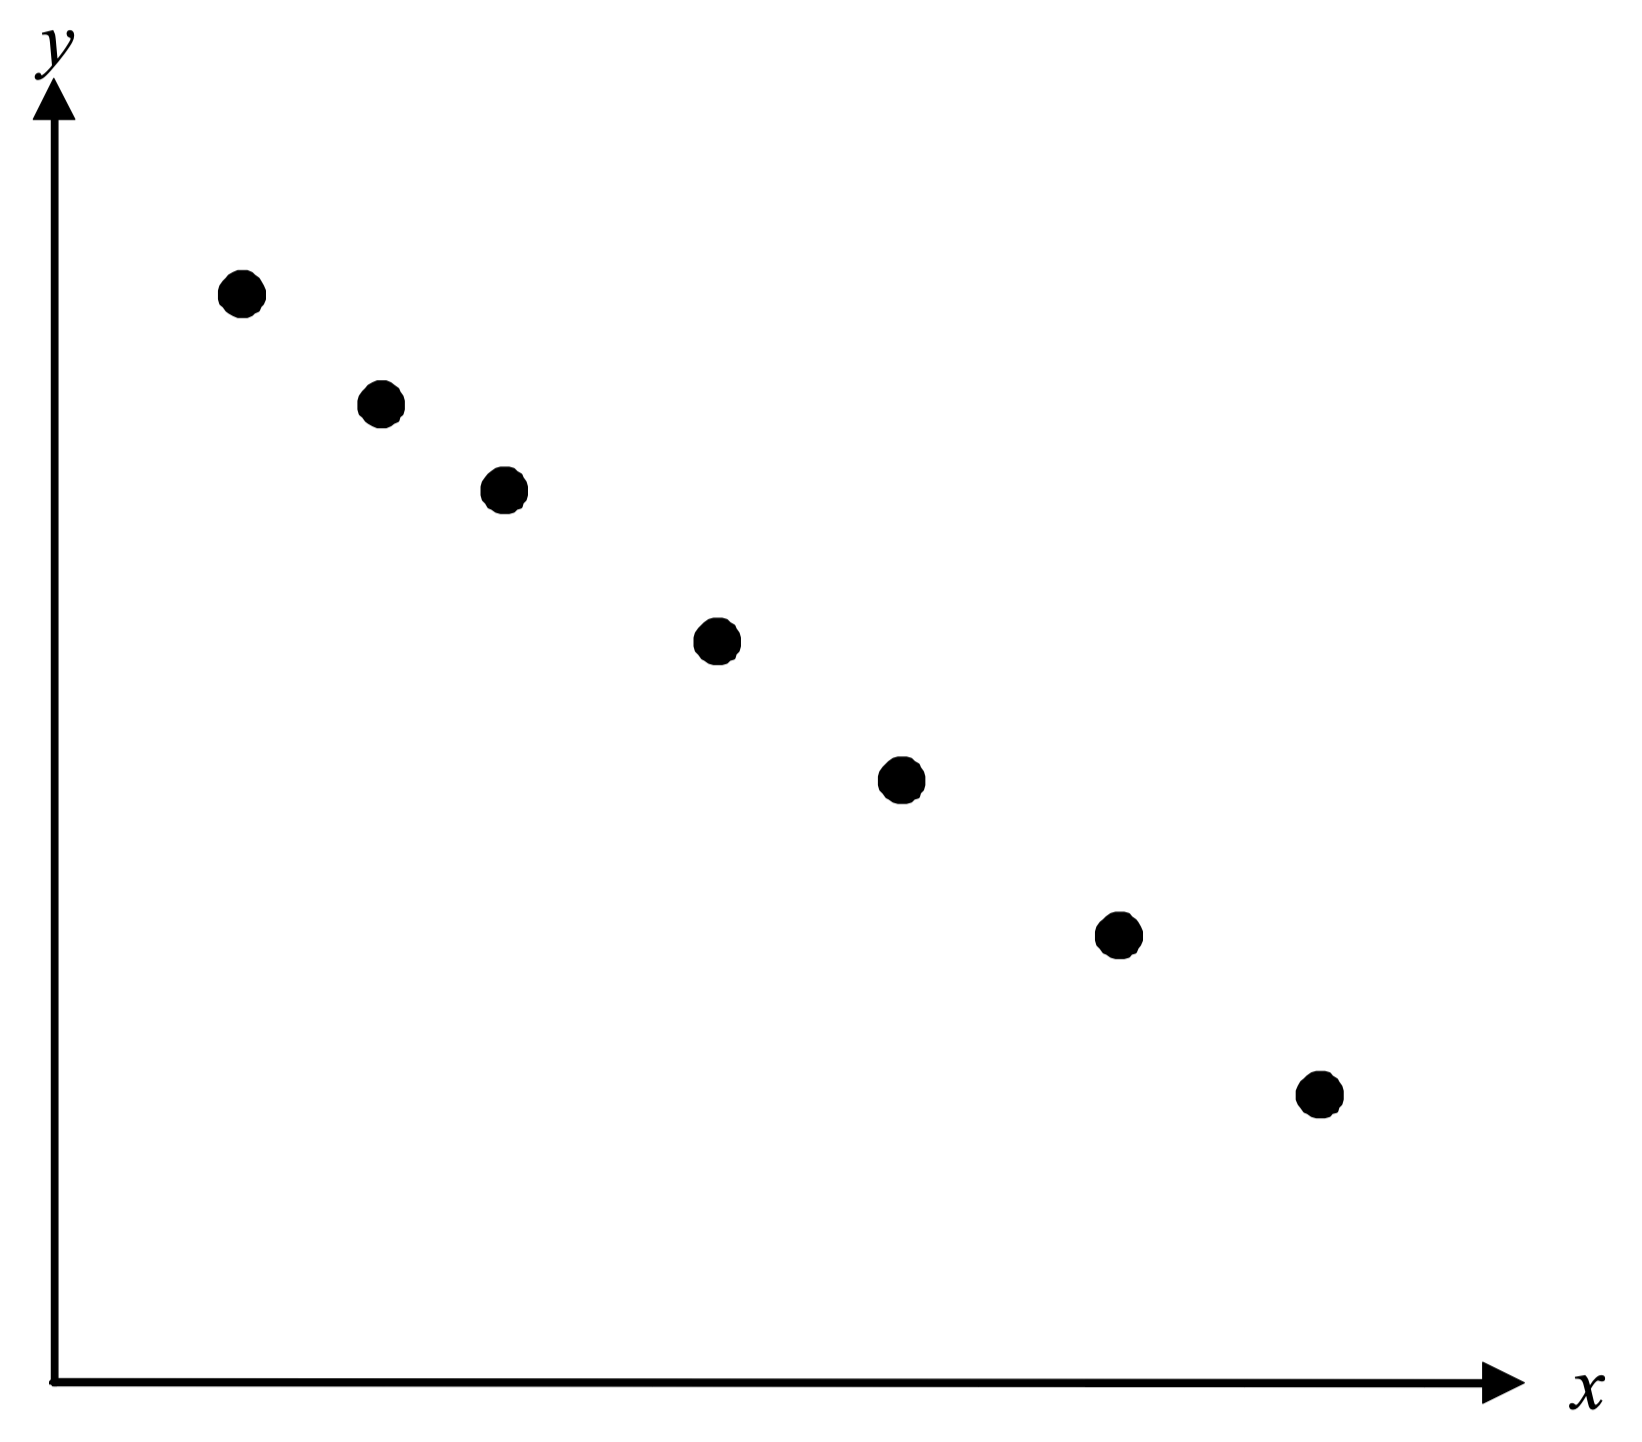
\includegraphics[width=0.45\textwidth,height=\textheight,keepaspectratio]{img/negative_correlation.png}
\caption{Correlazione lineare negativa}
\label{fig:negative_correlation}
\end{figure}
  \item si ha $r=0$ quando non esiste una relazione lineare tra i dati  (figura \ref{fig:no_correlation}).
  \begin{figure}[H]
\centering
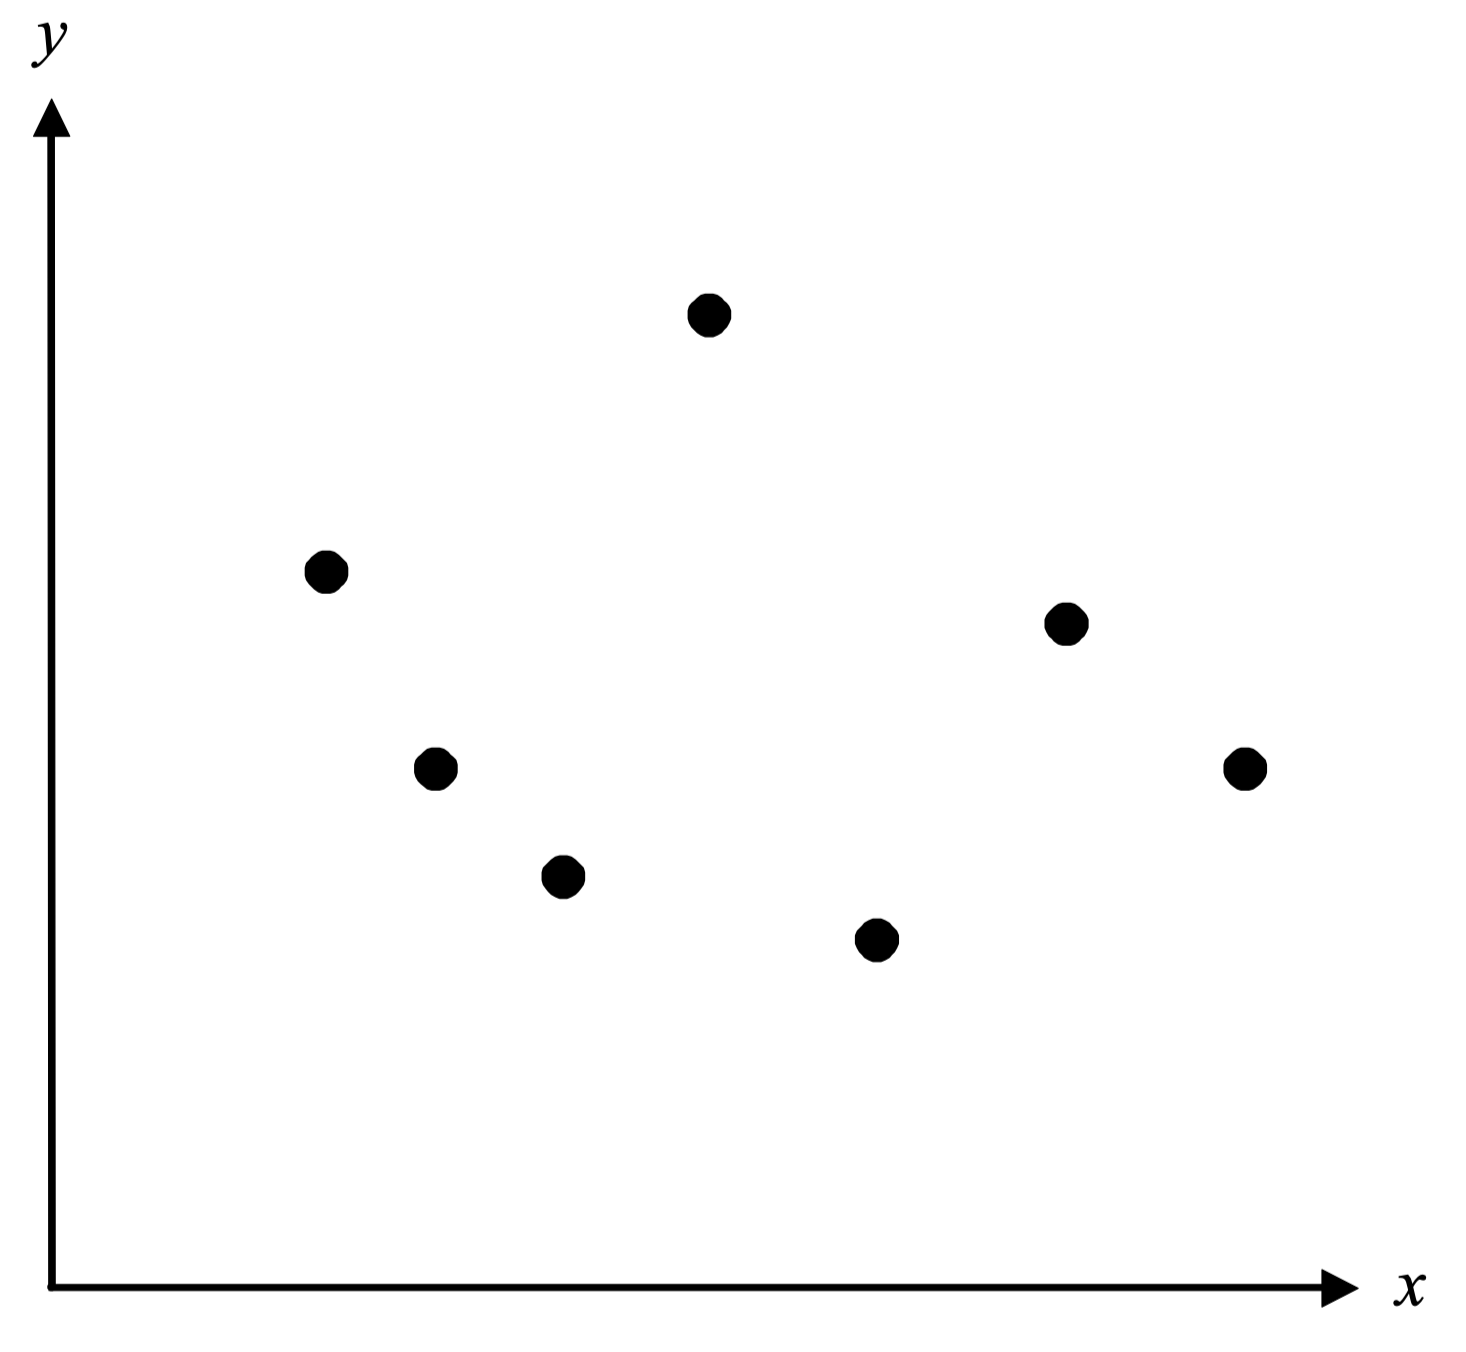
\includegraphics[width=0.45\textwidth,height=\textheight,keepaspectratio]{img/no_correlation.png}
\caption{Nessuna correlazione}
\label{fig:no_correlation}
\end{figure}
\end{itemize}

È noto che la varianza della variabile $Y$ ($\sigma_{y}^{2}$) si può scomporre in una parte ($\sigma_{\hat{y}}^{2}$), detta \textit{varianza spiegata}, in cui la variabilità della $Y$ è dovuta alla dipendenza di $Y$ dalla variabile $X$, e in una parte ($\sigma_{e}^{2}$), detta \textit{varianza non spiegata} in cui la  variabilità della $Y$ non dipende dalla variabile $X$, ma da altri fattori. Si può quindi introdurre un secondo indicatore, dato dal rapporto tra la varianza spiegata e la varianza totale, chiamato \textbf{coefficiente di determinazione}:

$$r^{2}=\frac{\sigma_{\hat{y}}^{2}}{\sigma_{y}^{2}}$$\smallskip

che indica quale frazione della variazione della variabile $Y$ può essere ricondotta e spiegata dalle variazioni della variabile $X$.

Sapendo che:

$$\sigma_{y}^{2}=\sigma_{\hat{y}}^{2}+\sigma_{e}^{2}$$

allora:

$$r^{2}=\frac{\sigma_{\hat{y}}^{2}}{\sigma_{\hat{y}}^{2}+\sigma_{e}^{2}}$$\smallskip

è evidente, quindi, che se la variabilità non spiegata è trascurabile, $\sigma_{e}^{2}$ tende ad annullarsi ed $r^{2}$ avrà un valore prossimo ad 1, mentre diventerà via via minore di 1 al diminuire dell’accordo tra la funzione calcolata e le osservazioni sperimentali.

Minore è la somma residua rispetto alla somma totale dei quadrati, maggiore sarà il valore del coefficiente di determinazione, $r^2$, il quale è un indicatore del livello di precisione con cui l'equazione ottenuta dall'analisi di regressione spiega la relazione tra le variabili. \cite{linear_models}\\

Un'altra metrica utile in ambito delle regressioni è l'errore quadratico medio (in inglese \textit{Mean Squared Error}, MSE) che indica la discrepanza quadratica media fra i valori dei dati osservati ed i valori dei dati stimati:

$$MSE=\frac{\sum_{i=1}^{n}\left(x_{i}-\widehat{x}_{i}\right)^{2}}{n}$$\smallskip

La sua radice quadrata fornisce un ulteriore indice statistico, la cosiddetta radice dell'errore quadratico medio (in inglese \textit{root-mean-square error}, RMSE). L'RMSE può essere anche calcolato come deviazione standard degli scarti. Da notare che l'MSE ed RMSE non sono quantità a-dimensionali, ma assumono l'unità di misura della grandezza considerata (RMSE) ed il suo quadrato (MSE). 

\subsection{Analisi dei residui}\label{ssec:regressione-residui}
Esistono metodi utili per diagnosticare le violazioni delle ipotesi di regressione di base: questi si basano principalmente sullo studio dei residui del modello. Spesso infatti la retta di regressione è una semplificazione della realtà e non coglie tutta la variabilità presente in un insieme di dati. \cite{residui_pozzolo}

Si definiscono i residui come:

$$e_{i}=y_{i}-\hat{y}_{i}, \quad i=1,2, \ldots, n$$\smallskip

dove $y_{i}$ è il valore osservato e $\hat{y}_{i}$ è il valore predetto.

Poiché un residuo può essere visto come la deviazione tra i dati e l'adattamento, è anche una misura della variabilità nella variabile di risposta, non spiegata dal modello di regressione. \cite{introduction_to_lr}

Eventuali scostamenti dalle ipotesi sugli errori dovrebbero quindi manifestarsi nei residui. L'analisi grafica dei residui è una tecnica efficace per verificare la linearità della relazione tra le variabili e  scoprire diversi tipi di inadeguatezze del modello, tra cui: 
\begin{itemize}
  \item se i residui hanno distribuzione normale (\ref{ssec:distr-errori});
  \item se gli errori non sono indipendenti rispetto ai valori di $X$ (\ref{ssec:correlazione-errore-variabili});
  \item se la varianza dei residui è omogenea (\ref{ssec:omogeneita-varianza});
  \item se ci sono degli outliers che influenzano la pendenza della retta (\ref{ssec:influenza-outliers}).
\end{itemize}

\subsubsection{Distribuzione degli errori}\label{ssec:distr-errori}
La distribuzione normale degli errori può essere verificata attraverso un grafico dei quantili, detto anche q-q plot.
In questa tipologia di grafico, i quantili teorici di una distribuzione Normale sono riportati sull’asse orizzontale. I quantili dei residui standardizzati sono invece riportati sull’asse verticale.
L’idea è che se i residui hanno una distribuzione normale, i loro quantili dovrebbero coincidere con quelli della distribuzione normale. A livello visivo, questo significa che i punti dovrebbero disporsi lungo la \textit{bisettrice}, indicata dalla retta presente nel grafico (figura \ref{fig:distr_errori}).

\begin{figure}[H]
\centering
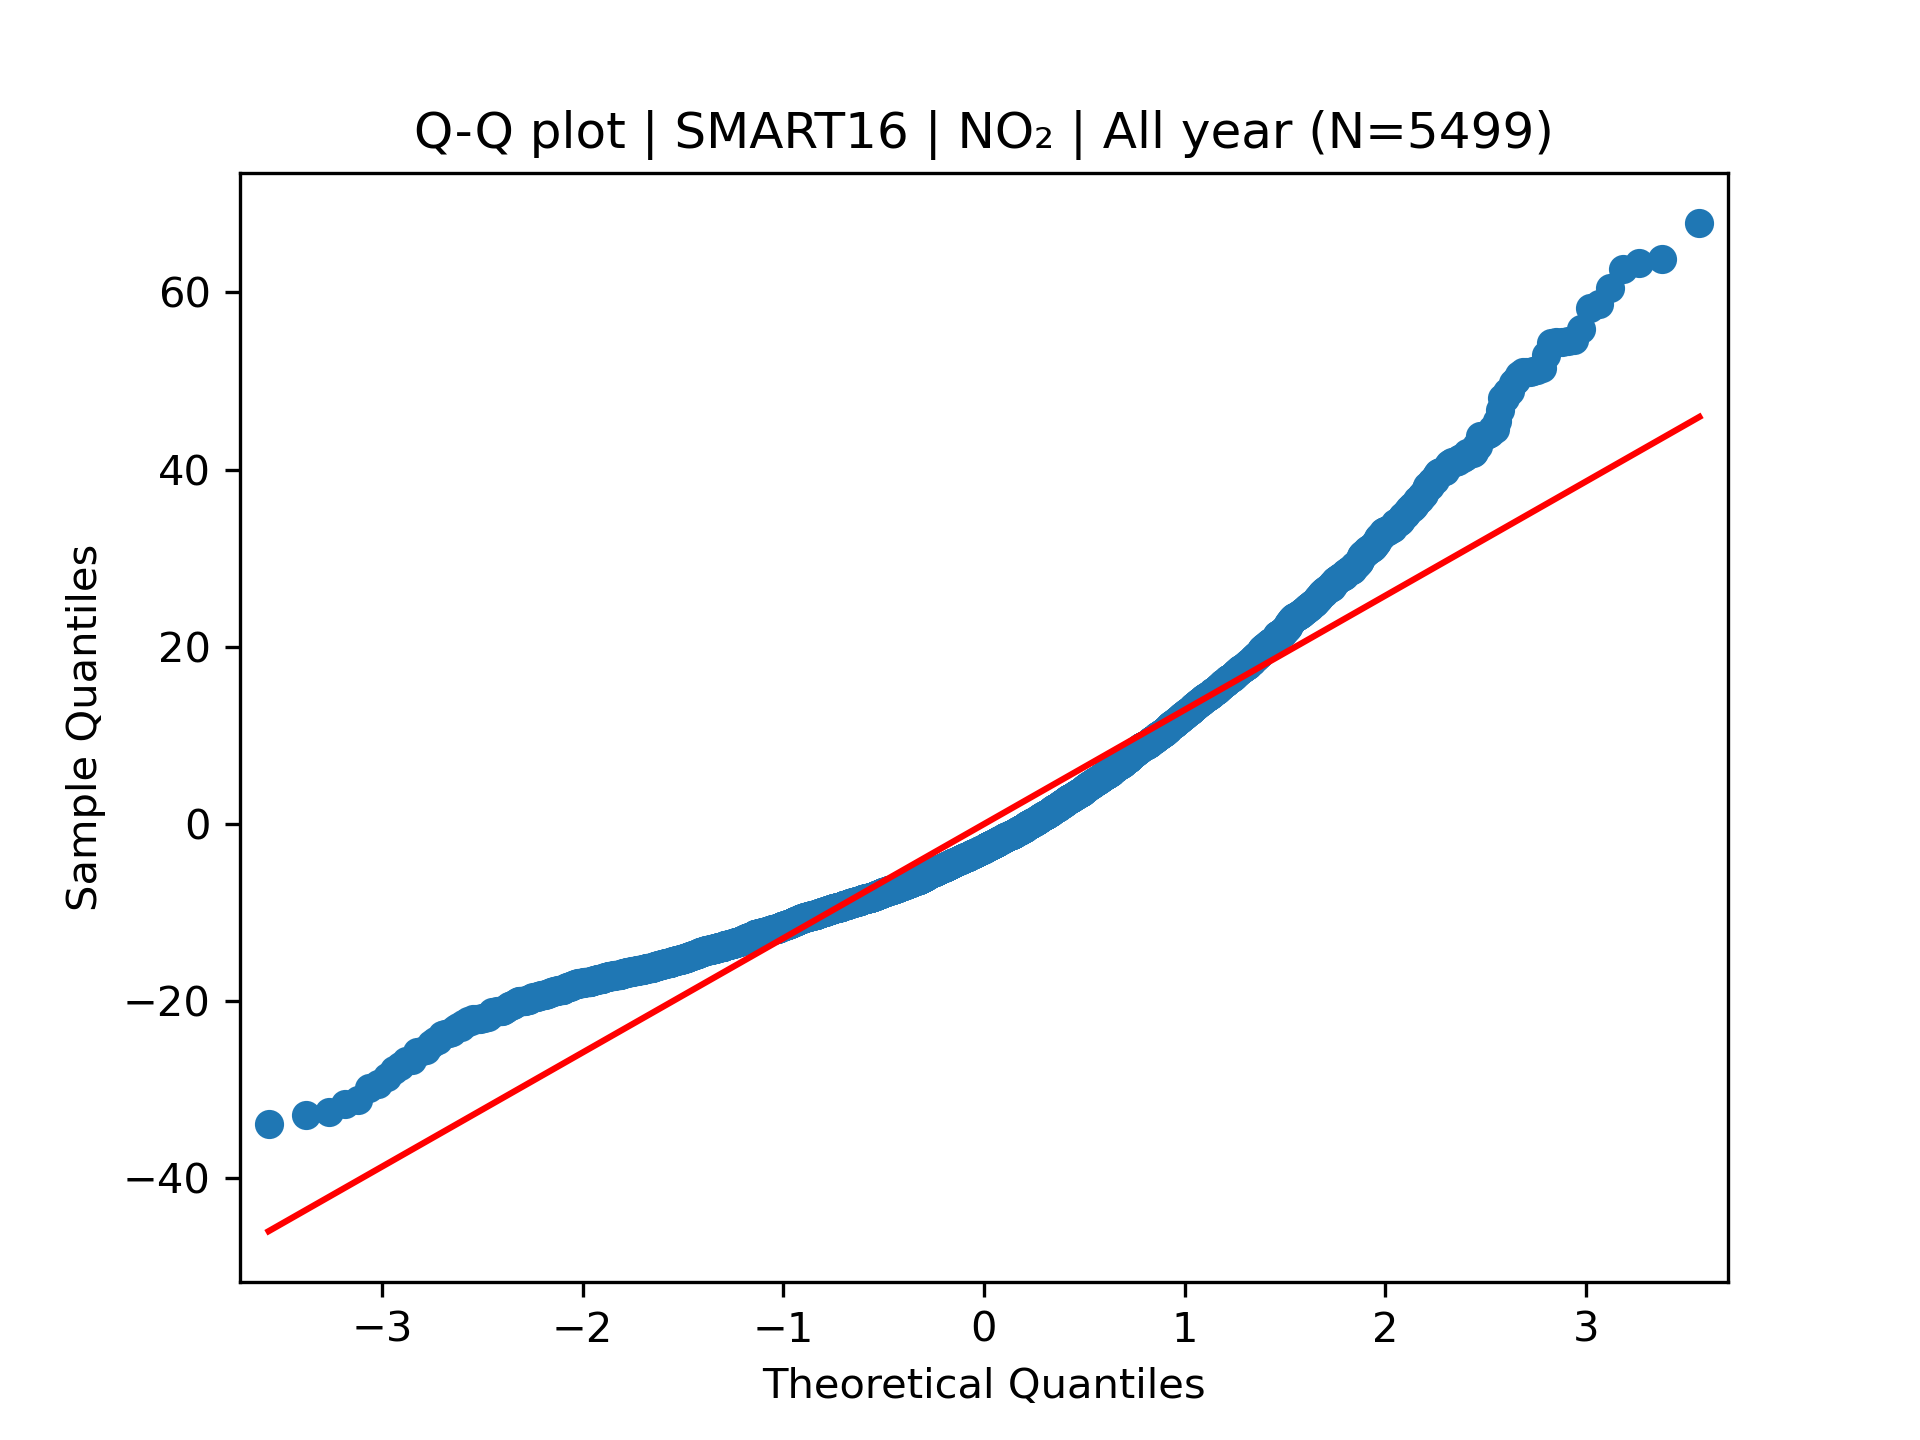
\includegraphics[width=0.65\textwidth,height=\textheight,keepaspectratio]{img/res_no2_qq}
\caption{Esempio di grafico distribuzione degli errori (q-q plot)}
\label{fig:distr_errori}
\end{figure}

Nella pratica, non capita quasi mai che i punti si dispongano esattamente lungo la bisettrice. Per poter dire che gli errori hanno una distribuzione normale ci si accontenta quindi che i punti siano vicino alla retta.

\subsubsection{Indipendenza degli errori}\label{ssec:correlazione-errore-variabili}
Se una variabile indipendente ($X$) risulta correlata con il termine d’errore, è possibile utilizzare questa variabile per predire quale sarà l’errore del modello di regressione. Questo in generale non è un buon segno, perché la componente di errore di un modello di previsione deve essere sempre imprevedibile.

Per verificare l'indipendenza tra la variabile indipendente e i residui è utile osservare un grafico come quello riportato in figura \ref{fig:residui-plot}, dove sull’asse orizzontale si riportano i valori della $x$ nell'ordine in cui sono stati raccolti, mentre sull’asse verticale i valori dei residui.

\begin{figure}[H]
\centering
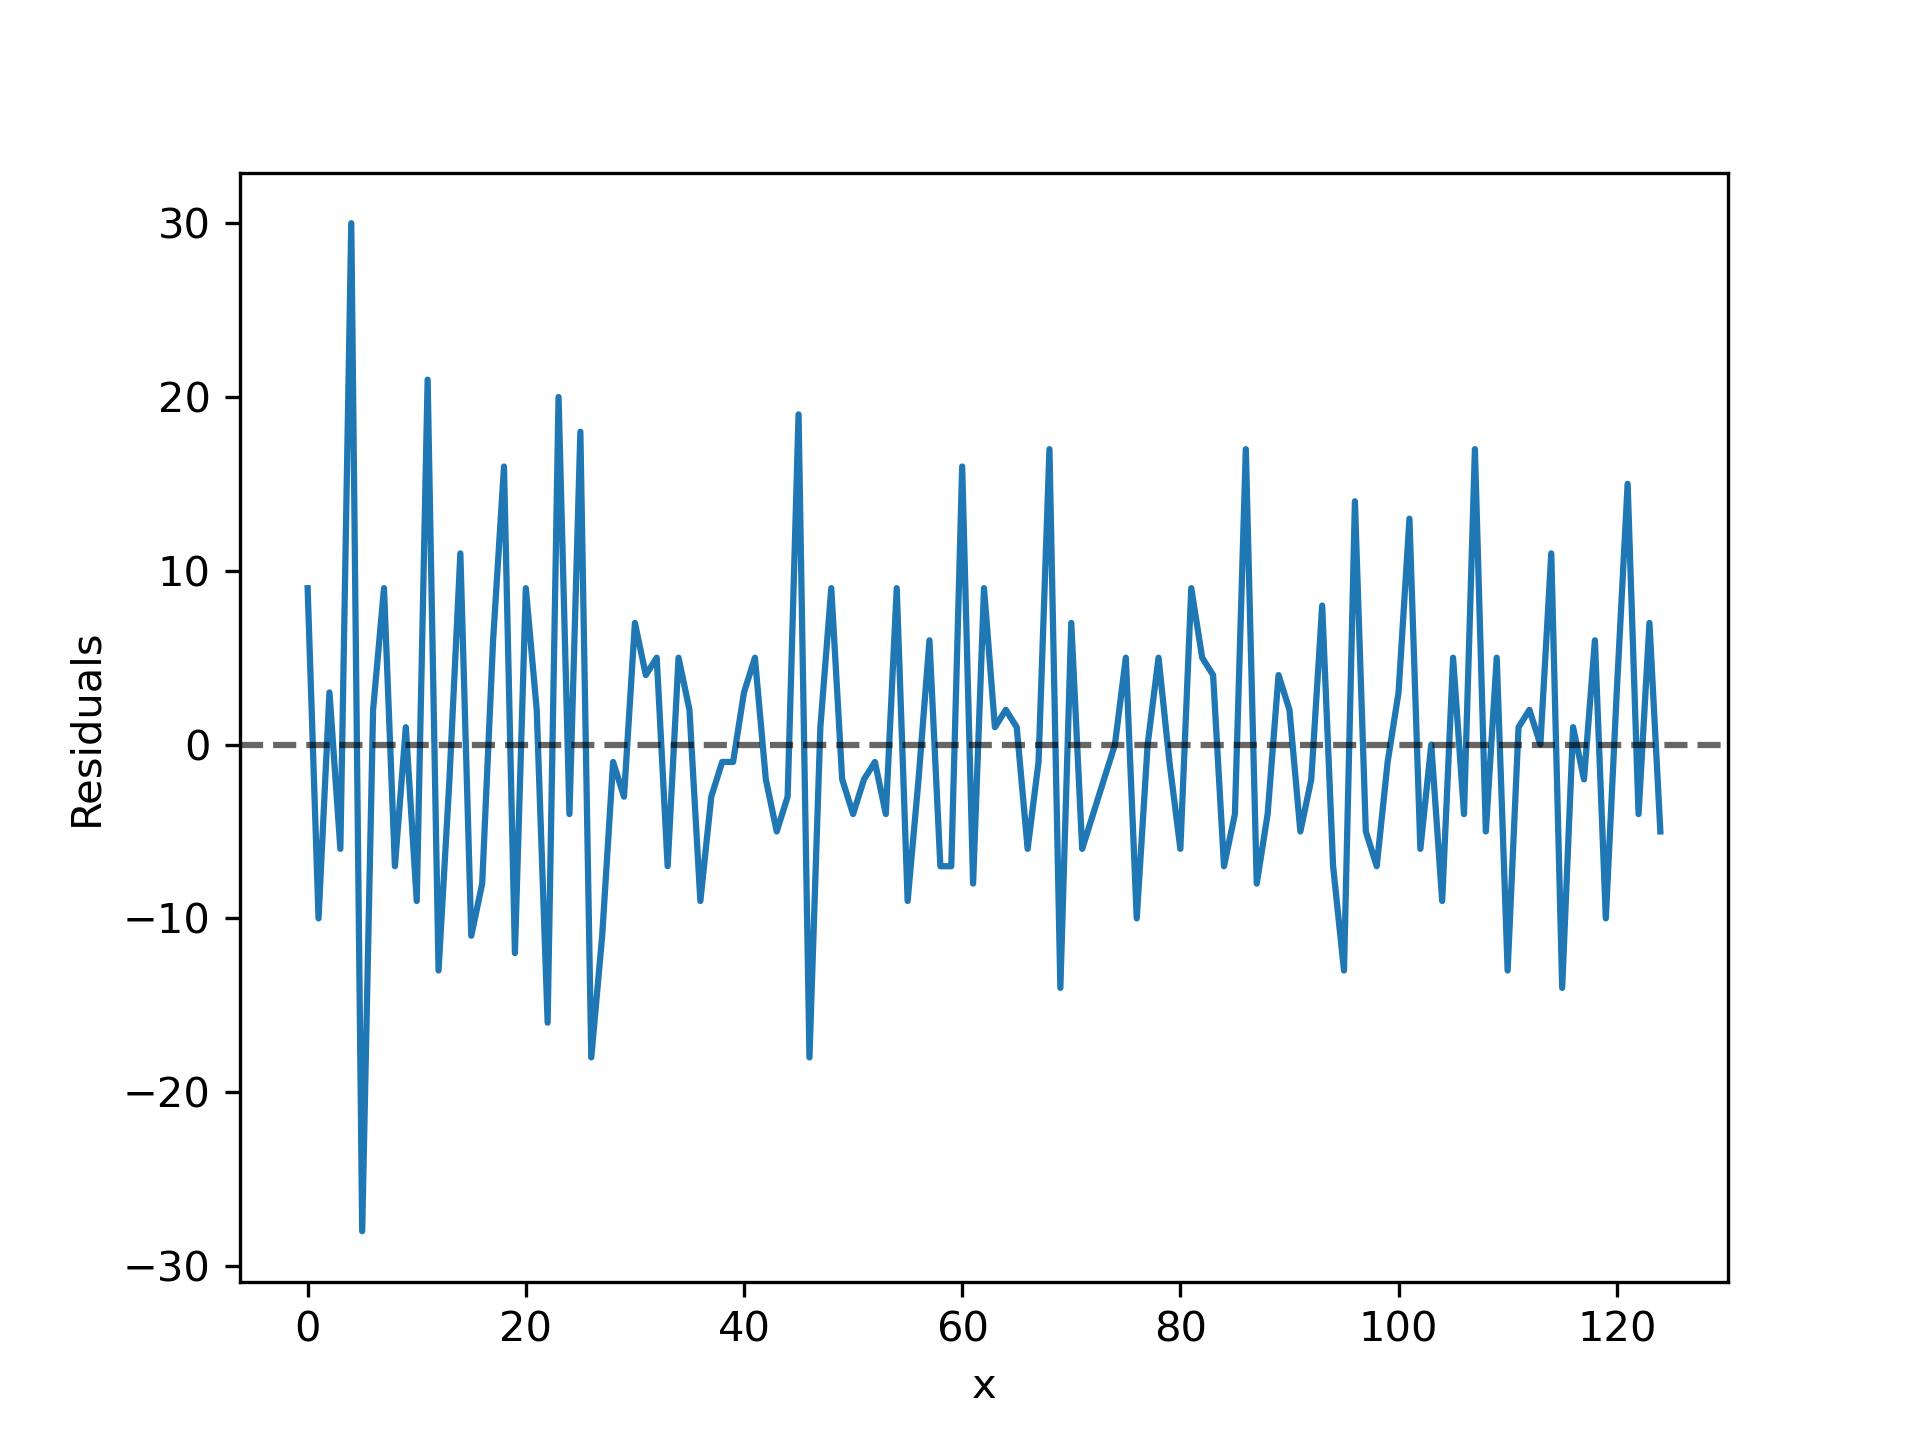
\includegraphics[width=0.65\textwidth,height=\textheight,keepaspectratio]{img/residual_plot}
\caption{Esempio di plot dei residui}
\label{fig:residui-plot}
\end{figure}

L’ipotesi è confermata se non è individuabile nessuna relazione tra le due variabili (ovvero se non compaiono trend o strutture cicliche nel tempo).

\subsubsection{Omogeneità della varianza dei residui}\label{ssec:omogeneita-varianza}
Per verificare l’ipotesi di omogeneità delle varianze dei residui, è necessario creare un grafico a dispersione (\textit{scatterplot}). I valori stimati della y si riportano sull’asse orizzontale delle $x$. Sull’asse verticale delle $y$ invece si indicano i valori dei residui (figura \ref{fig:distr_residui}).

\begin{figure}[H]
\centering
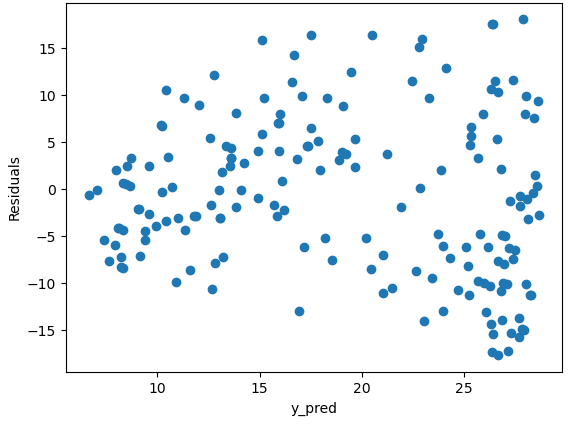
\includegraphics[width=0.65\textwidth,height=\textheight,keepaspectratio]{img/distr_residui.png}
\caption{Esempio di grafico distribuzione dei residui}
\label{fig:distr_residui}
\end{figure}

Se c’è omogeneità della varianza dei residui, i punti saranno dispersi in modo simile sia nella parte sinistra che in quella destra del grafico. Questa proprietà se verificata prende il nome di \textbf{omoschedasticità}.

\subsubsection{Influenza di outliers}\label{ssec:influenza-outliers}
Il grafico a dispersione tra valori predetti e residui permette di individuare anche i possibili \textit{outliers}, ovvero i punti isolati nel grafico (quelli con residui maggiori).
Tuttavia, per verificare se ci sono outliers in un modello di regressione, spesso si utilizzano altre tecniche (ad esempio eliminando i punti problematici tramite la distanza di Cook, descritta in \ref{sssec:regressione-cook}, oppure applicando stime robuste meno sensibili alle le osservazioni problematiche, ad esempio con la funzione peso di Huber  descritta in \ref{sssec:regressione-huber}). Nel primo caso è utile anche provare a rifare le analisi di regressione escludendo le osservazioni potenzialmente problematiche e vedere se ci sono differenze nei coefficienti del modello.

Nei modelli di regressione infatti anche un singolo outlier può influenzare in maniera sostanziale la capacità di adattamento del modello ai dati, soprattutto se il campione non risulta molto numeroso.

\subsection{Modelli di regressione}\label{ssec:regressione-modelli}
I modelli di regressione sono ampiamente utilizzati sia per la previsione o la descrizione dei dati che per la stima e il controllo dei parametri.

\subsubsection{Regressione lineare}\label{sssec:regressione-lineare}
Considerata una funzione lineare a due variabili:
$$y = a + b*x$$

In questo caso si deve rendere minima la funzione:

$$\varphi(a, b)=\sum_{i=1}^{n}\left[y_{i}-\left(a+b x_{i}\right)\right]^{2}$$\smallskip

Annullando le derivate parziali prime rispetto ad $a$ e $b$ si ha il sistema:

$$\left\{\begin{array}{l}
\sum_{i=1}^{n} 2\left[y_{i}-\left(a+b x_{i}\right)\right](-1)=0 \\
\sum_{i=1}^{n} 2\left[y_{i}-\left(a+b x_{i}\right)\right]\left(-x_{i}\right)=0
\end{array}\right.$$\smallskip

che risolto, fornisce i valori dei parametri:

$$\left\{\begin{array}{l}
\hat{a}=\bar{y}-b \bar{x} \\
\hat{b}=\frac{\sum_{i=1}^{n}\left(x_{i}-\bar{x}\right)\left(y_{i}-\bar{y}\right)}{\sum_{i=1}^{n}\left(x_{i}-\bar{x}\right)^{2}}
\end{array}\right.$$\smallskip

dove $\bar{x}$ e $\bar{y}$ indicano le \textit{medie aritmetiche}, rispettivamente di $x_i$ e $y_i$.

La stima del parametro $b$, \textit{coefficiente angolare} della funzione lineare, può essere rappresentato nella forma:

$$\hat{b}=\frac{\sum_{i=1}^{n} \frac{\left(x_{i}-\bar{x}\right)\left(y_{i}-\bar{y}\right)}{n}}{\sum_{i=1}^{n} \frac{\left(x_{i}-\bar{x}\right)^{2}}{n}}$$\smallskip

dove il denominatore è la \textit{varianza} di $X$ ($\sigma_{X}^{2}$), mentre il numeratore è detto \textit{covarianza} di X e Y ($\sigma_{XY}$) e misura la variabilità congiunta delle coppie ($x_i$, $y_i$) di valori corrispondenti rispetto al proprio valor medio; quindi, il coefficiente $b$ della retta interpolante esprime la variabilità congiunta di $X$ e $Y$ rapportata alla variabilità della sola $X$. \cite{Neter1996}

\begin{figure}[H]
\centering
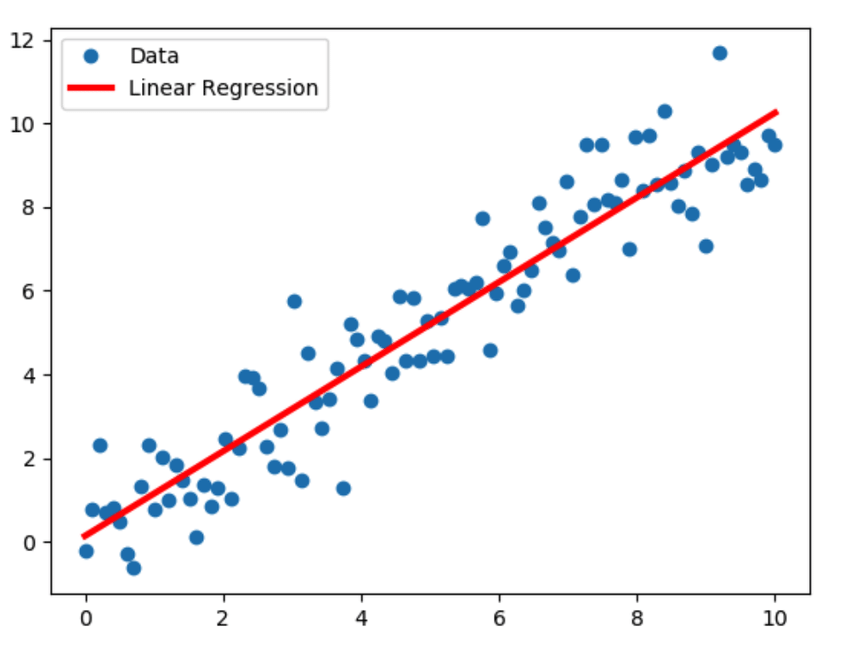
\includegraphics[width=0.65\textwidth,height=\textheight,keepaspectratio]{img/lin_reg_example.png}
\caption{Esempio di regressione lineare}
\label{fig:reg_lin}
\end{figure}

La precisione della retta calcolata dalla regressione lineare dipende dal grado di dispersione nei dati. Più i dati sono lineari, più il modello risulterà accurato.

%Per stimare la relazione tra due variabili, la regressione lineare utilizza una formula matematica che calcola la media dei valori della prima variabile (Y) in funzione dei valori della seconda variabile (X). La formula della regressione lineare è:
%
%Y = a + bX
%
%In questa formula, a è la costante di regressione e b è la coefficiente di regressione. La costante di regressione a indica la media dei valori di Y in funzione dei valori di X. Il coefficiente di regressione b indica la relazione tra le due variabili: più è vicino a 1, più le due variabili sono correlate in modo lineare.
%
%Utilizzando la regressione lineare, è possibile stimare la relazione tra due variabili anche in presenza di deviazioni dalla linea.

\subsubsection{Regressione lineare robusta (Huber)}\label{sssec:regressione-huber}
La regressione Huber (in inglese Huber regression, anche detta regressione robusta) è una metodologia statistica per la stima dei parametri di un modello lineare in presenza di \textit{outliers}.

Ci sono situazioni in cui si verifica presenza di valori anomali che influiscono sul modello di regressione, nel senso che possono avere una forte influenza sul metodo dei minimi quadrati, di fatto \textit{deviando} troppo l'equazione di regressione nella loro direzione. Il metodo dei minimi quadrati, infatti, in questi casi ha lo svantaggio di avere la tendenza ad essere dominato da questi valori — infatti sommando il quadrato dei residui ($\sum_{i=1}^{n} a_i^2$ dove $a_i$ è il residuo i-esimo), la media risulta troppo influenzata da pochi valori $a_i$ particolarmente grandi.

Ci sono due modi per affrontare questa situazione:

\begin{itemize}
  \item Scartare le osservazioni \textit{scomode} (vedi regressione lineare avanzata \ref{sssec:regressione-cook});
  \item Applicare procedure di stime robuste in modo che siano meno sensibili alle osservazioni troppo influenti (figura \ref{fig:reg_rob}).
\end{itemize}

\begin{figure}[H]
\centering
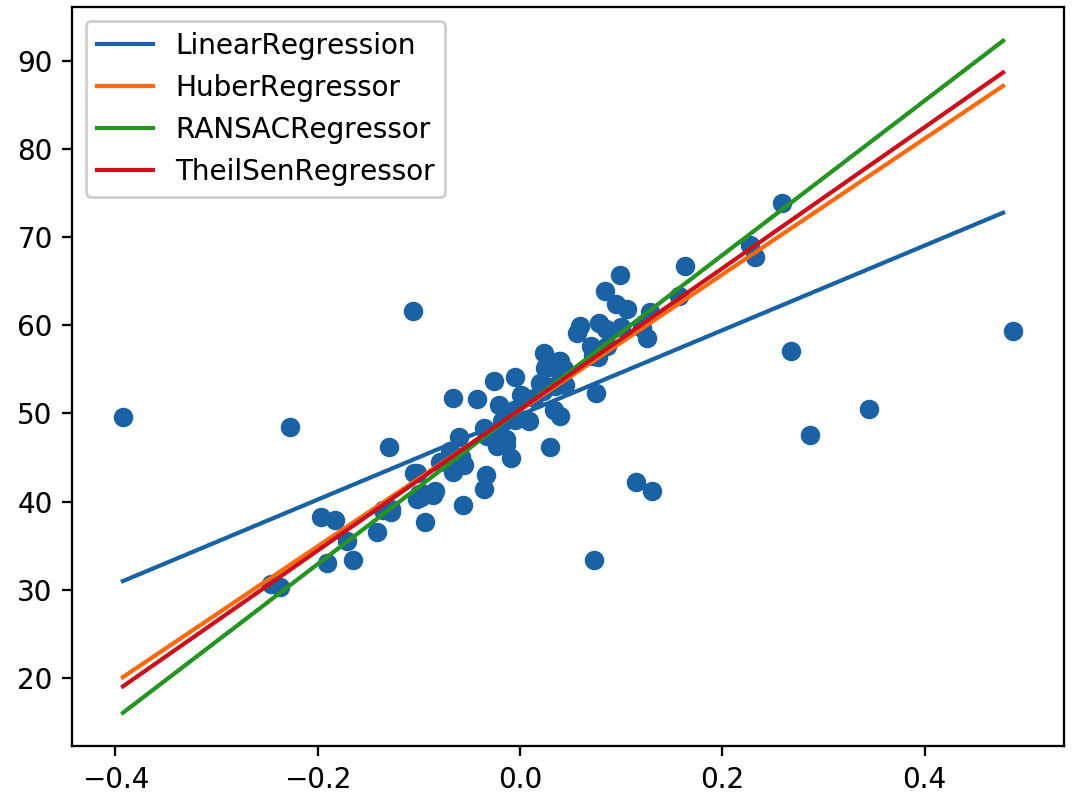
\includegraphics[width=0.55\textwidth,height=\textheight,keepaspectratio]{img/robust.png}
\caption{Comportamento di modelli di regressione robusta in presenza di outliers}
\label{fig:reg_rob}
\end{figure}

Una delle funzioni di stima robusta, comunemente usata in diversi metodi di regressione per ridurre la sensibilità dei parametri alla presenza di outliers, è la \textbf{funzione di Huber}, appartenente ad una classe di estimatori denominata \textbf{M-estimator}, e che risulta quadratica per piccoli valori di $x$, e lineare per valori più grandi. È definita come:

$$L_{\delta}(a)= \begin{cases}\frac{1}{2} a^{2} & \text { per }|a| \leq \delta \\ \delta\left(|a|-\frac{1}{2} \delta\right), & \text { altrimenti }\end{cases}$$\smallskip

Dove la variabile $a$ fa riferimento al residuo, cioè la differenza tra valore osservato e valore predetto ($a = y - f(x)$).


\subsubsection{Regressione lineare avanzata}\label{sssec:regressione-cook}
Come accennato in \ref{sssec:regressione-huber}, un'altra tecnica per la gestione di outlier è quella di applicare il modello sul dataset dopo aver rimosso i valori anomali. Esistono molte metriche su cui basarsi per rimuovere gli outlier da un set di dati: un metodo che viene spesso utilizzato nella regressione è la \textbf{distanza di Cook}.

La distanza di Cook è una stima dell'\textit{influenza} di una osservazione in un dataset, in termini di residuo (outlier) o di elevato \textit{leverage}: è un riepilogo di quanto cambierebbe un modello di regressione nel caso in cui venga rimossa l'i-esima osservazione.\\

In presenza di outliers la distanza di Cook aumenta, e quindi questi dati ad alta influenza hanno un maggiore impatto sulle stime dei parametri della regressione.\\

La distanza di Cook \cite{cook_def} dell'osservazione $i$ ($\forall i=1, \ldots, n$) è definita come:

$$D_{i}=\frac{\sum_{j=1}^{n}\left(\hat{y}_{j}-\hat{y}_{j(i)}\right)^{2}}{p s^{2}}$$\smallskip

dove:

\begin{itemize}
  \item $n$ è il numero di osservazioni;
  \item $\hat{y}_{j}$ è il valore predetto;
  \item $\hat{y}_{j(i)}$ è la risposta ottenuta escludendo l'i-esima osservazione.
\end{itemize}

Oppure, in modo equivalente:

$$D_{i}=\frac{e_{i}^2}{p s^{2}}\left[\frac{h_{i}}{\left(1-h_{i}\right)^{2}}\right]$$\smallskip

dove:

\begin{itemize}
  \item $e_{i} = y_i - \hat{y_i}$  è l'i-esimo residuo;
  \item $p$ è il numero di coefficienti della regressione;
  \item $s^2$ è l'errore quadratico medio (MSE);
  \item $h_i$ è il peso che l'i-esimo osservazione ha sul valore della regressione (\textit{leverage}).
\end{itemize}

Un esempio di rilevazione grafica di outlier tramite distanza di Cook è riportato in figura \ref{fig:cook}.

\begin{figure}[H]
\centering
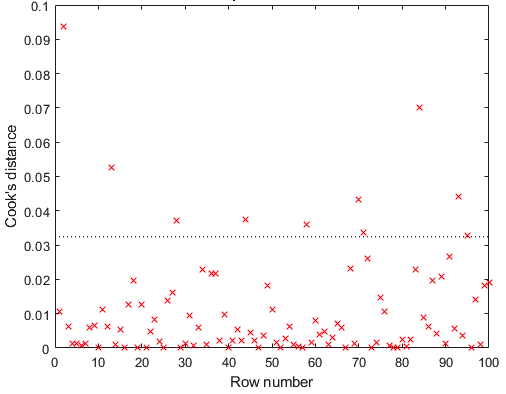
\includegraphics[width=0.65\textwidth,height=\textheight,keepaspectratio]{img/cook.png}
\caption{Riconoscimento di outlier tramite distanza di Cook}
\label{fig:cook}
\end{figure}

Vi sono diverse opinioni riguardo al valore di soglia di \textit{cut-off}, oltre la quale un dato può essere considerato un outlier. In \cite{applied_regression} viene proposta:

$$D_{i}>\frac{4}{n}$$\smallskip

dove $n$ è il numero di osservazioni. La distanza di Cook può anche essere utilizzata per individuare regioni dello spazio nelle quali sarebbe necessario effettuare una validazione, ad esempio acquisendo più dati.

\subsubsection{Regressione Ridge}\label{sssec:regressione-ridge}
Nella statistica e nel Machine Learning, la regressione Ridge è un metodo di analisi di regressione che applica una fase di \textbf{regolarizzazione} al fine di migliorare l'accuratezza della previsione, prevenire l'\textit{overfitting} e penalizzare la complessità del modello.
Insieme al LASSO (vedi \ref{sssec:regressione-lasso}) è un modello di regressione che viene ripreso anche da tecniche di Boosting di Machine Learning. In generale esistono due tipi di penalizzazione:
\begin{itemize}
  \item \textbf{L1}: penalizza il valore assoluto dei coefficienti del modello (es. Lasso); 
  \item \textbf{L2}: penalizza il quadrato del valore dei coefficienti del modello (es. Ridge).
\end{itemize}

La regressione Ridge usa la penalità L2: in pratica questo produce coefficienti piccoli, ma nessuno di loro è mai annullato (\textit{feature shrinkage}).

Richiamando il metodo dei minimi quadrati (\ref{ssec:regressione-introduzione}) si deve minimizzare la somma dei quadrati dei residui (RSS):

$$\mathrm{RSS}=\sum_{i=1}^{n}\left(y_{i}-\beta_{0}-\sum_{j=1}^{p} \beta_{j} x_{i j}\right)^{2}$$\smallskip

Nella regressione Ridge si aggiunge anche un termine di penalità, ottenendo quindi:

$$\sum_{i=1}^{n}\left(y_{i}-\beta_{0}-\sum_{j=1}^{p} \beta_{j} x_{i j}\right)^{2}+\lambda \sum_{j=1}^{p} \beta_{j}^{2}=R S S+\lambda \sum_{j=1}^{p} \beta_{j}^{2}$$\smallskip

Dove $\lambda$ è un parametro di \textit{tuning} che serve proprio a controllare l’effetto della penalità: un valore $\lambda=0$ infatti non avrà effetto sul risultato finale (l’equazione viene ricondotta a quella dei minimi quadrati), al contrario per $\lambda \to \infty$ invece i coefficienti di regressione stimati tenderanno a zero poiché si darà molto peso alla penalità del modello. \cite{lasso_vs_ridge}

Il modello di regressione di Ridge presenta dei vantaggi rispetto a quello dei minimi quadrati, soprattutto per quanto riguarda il \textit{bias-variance trade-off}: in generale, quando c’è una relazione lineare tra i predittori e la variabile risposta, il modello dei minimi quadrati comporta poco bias ma alta varianza. Questo si traduce nel fatto che una piccola variazione nell'ooservazione può generare un cambiamento notevole nei coefficienti stimati. \cite{tesi_polito}

\subsubsection{Regressione Lasso}\label{sssec:regressione-lasso}
Lo svantaggio della regressione Ridge è il fatto di considerare tutte le variabili per la predizione nel modello finale. Il termine di regolarizzazione $\lambda \sum_{j=1}^{p} \beta_{j}^{2}$ tende ad assegnare ai coefficienti valori vicini allo zero, ma non perfettamente zero, a meno che $\lambda = 0$.
Questo crea problemi non tanto per l’accuratezza della predizione, ma per l’interpretazione delle varabili, soprattutto quando il numero di queste diventa alto.

La regressione Lasso (acronimo di \textit{least absolute shrinkage and selection operator}, ovvero operatore di restringimento e selezione minimo assoluto) è un’alternativa alla regressione Ridge utilizzata proprio per superare questo problema. L'unica differenza sta nel termine di regolarizzazione, ovvero:

$$\lambda \sum_{j=1}^{p}\left|\beta_{j}\right|$$\smallskip

Per cui l'equazione del modello diventa:

$$\sum_{i=1}^{n}\left(y_{i}-\beta_{0}-\sum_{j=1}^{p} \beta_{j} x_{i j}\right)^{2}+\lambda \sum_{j=1}^{p}\left|\beta_{j}\right|=R S S+\lambda \sum_{j=1}^{p}\left|\beta_{j}\right|$$\smallskip

Anche nel caso di regressione Lasso il parametro di regolarizzazione tende a stimare i valori dei coefficienti verso lo zero ma, a differenza della regressione Ridge, la penalità $\lambda \sum_{j=1}^{p}\left|\beta_{j}\right|$ costringe uno o più coefficienti ad essere esattamente zero per certi valori di $\lambda$. \cite{tesi_polito}

\subsubsection{Regressione polinomiale}\label{sssec:regressione-polinomiale}
La regressione polinomiale è una generalizzazione della regressione lineare, infatti utilizza lo stesso metodo matematico della variante lineare, ma assume che la relazione di funzione che caratterizza i dati sia meglio descritta, anzichè da una retta, da un polinomio. In questo caso il metodo dei minimi quadrati può essere utilizzato anche per adattare una funzione polinomiale a un insieme di dati. Considerato un polinomio di grado $k$:

$$y=a_{0}+a_{1} x+a_{2} x^{2}+a_{3} x^{3}+\ldots+a_{k} x^{k}$$\smallskip

In questo caso il sistema di equazioni da risolvere è:

$$\left\{\begin{array}{l}
n a_{0}+a_{1} \sum_{i=1}^{n} x_{i}+a_{2} \sum_{i=1}^{n} x_{i}^{2}+\cdots+a_{k} \sum_{i=1}^{n} x_{i}^{k}=\sum_{i=1}^{n} y_{i} \\
a_{1} \sum_{i=1}^{n} x_{i}+a_{2} \sum_{i=1}^{n} x_{i}^{2}+\cdots+a_{k} \sum_{i=1}^{n} x_{i}^{k}=\sum_{i=1}^{n} x_{i} y_{i} \\
\cdots \\
a_{1} \sum_{i=1}^{n} x_{i}^{k}+a_{2} \sum_{i=1}^{n} x_{i}^{k+1}+\cdots+a_{k} \sum_{i=1}^{n} x_{i}^{2 k}=\sum_{i=1}^{n} x_{i}^{k} y_{i}
\end{array}\right.$$\smallskip

che, risolto, permette di ricavare i parametri $a_0$, $a_1$, $a_2$, ..., $a_k$.

\begin{figure}[H]
\centering
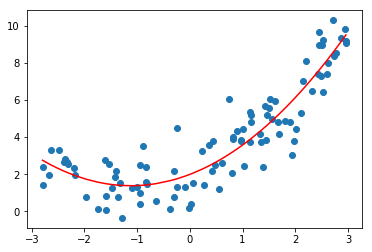
\includegraphics[width=0.55\textwidth,height=\textheight,keepaspectratio]{img/poly_reg_example.png}
\caption{Esempio di regressione polinomiale}
\label{fig:poly_reg}
\end{figure}

Ci sono diverse considerazioni importanti che emergono quando si adatta un polinomio in una variabile: una di queste riguarda la scelta dell'ordine del modello.
Come regola generale, l'uso di polinomi di ordine elevato ($n > 3$) dovrebbe essere evitato: un modello di ordine basso è quasi sempre preferibile a un modello di ordine elevato per ragioni di minore complessità, di coerenza con i dati e per evitare \textit{overfitting}.

Come caso estremo, è sempre possibile trovare un polinomio di grado $n-1$ ad $n$ punti che risulti in un buon adattamento dei dati.
Nella maggior parte dei casi, però, questo non farebbe nulla per migliorare la comprensione della funzione sconosciuta, né sarebbe probabilmente un buon predittore.

\subsubsection{Regressione con Random Forest}\label{sssec:regressione-rf}
La regressione Random Forest è un algoritmo di apprendimento supervisionato che utilizza il metodo di apprendimento \textit{ensemble} per la regressione tramite alberi di decisione. Il metodo di apprendimento ensemble è una tecnica che combina le previsioni di più algoritmi di apprendimento automatico per effettuare una previsione più accurata rispetto a un singolo modello. \cite{random_forest}

In particolare, una foresta casuale (random forest) opera adattando una serie di alberi decisionali su vari sottocampioni del set di dati e utilizza la media dei risultati per migliorare l'accuratezza predittiva e controllare l'overfitting.
In breve, l'algoritmo funziona eseguendo i seguenti passi:

\begin{enumerate}
  \item Sceglie a caso $k$ osservazioni dati dal training set;
  \item Costruisce un albero decisionale associato a queste $k$ osservazioni;
  \item Sceglie il numero $N$ di alberi da costruire e ripete i passaggi 1 e 2 per ciascuno;
  \item Per una nuova osservazione, fa in modo che ciascuno degli $N$ alberi preveda il valore di $y$, e assegna il nuovo punto alla media su tutti i valori $y$ previsti.
\end{enumerate}

Uno dei principali svantaggi degli alberi decisionali è che risultano molto inclini a provocare \textit{overfitting}: funzionano bene sui dati di training, ma non sono così flessibili per fare previsioni su campioni non visti in precedenza. Sebbene esistano soluzioni alternative per migliorare questo aspetto, come ad esempio ridurre il numero di alberi, questo riduce il loro potere predittivo. Generalmente sono modelli con \textit{bias} medio e varianza alta, ma sono semplici e di facile interpretazione.

\subsubsection{Regressione con Gradient Boosting}\label{sssec:regressione-gb}
Il Gradient Boosting è una tecnica di Machine Learning che ha alla base la stima iterativa di alberi sui residui ottenuti ad ogni passo e l’aggiornamento in maniera adattiva delle stime. Questa tecnica riprende il concetto matematico del \textit{gradient descent}, per cui lo split scelto sarà quello che favorisce l’avvicinamento al punto di minimo della funzione obiettivo.

Il \textit{gradient descent} è un algoritmo di ottimizzazione che consente di individuare il valore minimo di una funzione di costo per sviluppare un modello con una previsione accurata.

L’algoritmo Gradient Boosting applicato a problemi di regressione può essere descritto nei seguenti passi:

\begin{enumerate}
  \item Si inizializza il modello con un valore noto;
  \item Si considera sul training set una \textit{loss function}, ovvero una funzione differenziabile che esprima una valutazione della predizione (es. $\frac{1}{2} (y_i - \hat{y}_{i})$ dove $y_i$ è l'osservazione e $\hat{y}_{i}$ è la predizione);
  \item Scelto un numero massimo, si itera modellando un albero di regressione seguendo una procedura di discesa del gradiente, in modo da minimizzare la \textit{loss function}. L'albero ottenuto viene aggiunto alla sequenza di alberi già esistente, nel tentativo di correggere o migliorare l'output finale del modello.
\end{enumerate}


\subsubsection{Regressione con SVR}\label{sssec:regressione-svr}
Un altro modello per la regressione è SVR (\textit{support-vector regression}), basato sui modelli SVM (support-vector machines) di apprendimento supervisionato, spesso impiegati nel problema della classificazione. \cite{svm}

Rispetto alla regressione lineare e al metodo dei minimi quadrati, SVR presenta più flessibilità perchè consente di definire una soglia di accettazione dell'errore nel modello. Infatti l'agoritmo SVR si propone di minimizzare non l'errore quadratico, come nel metodo dei minimi quadrati, ma i coefficienti (nello specifico, la norma al quadrato del vettore dei coefficienti). La funzione obiettivo quindi diventa:

$$min \frac{1}{2}\|\mathbf{w}\|^{2}$$\smallskip

 Il termine di errore invece è gestito nei vincoli, dove si imposta l'errore assoluto minore o uguale a un margine specificato, chiamato errore massimo ($\varepsilon$):
 
 $$\left|y_{i}-w_{i} x_{i}\right| \leq \varepsilon$$\smallskip
 
 Il tuning del parametro $\varepsilon$ consente di ottenere la precisione desiderata del modello di regressione. Solitamente alla funzione obiettivo si aggiunge anche delle variabili di \textit{slack} ($\xi_{i}$), che indicano la deviazione dal margine di ciascun valore che supera la soglia $\varepsilon$ (lo scopo è di minimizzarle il più possibile). La funzione obiettivo in questo caso diventa:
 
 $$min \frac{1}{2}\|\mathbf{w}\|^{2} + C \sum_{i=1}^{n}\left|\xi_{i}\right|$$\smallskip

dove $C$ è un altro iperparametro regolabile: all'aumentare di $C$, aumenta anche la tolleranza per i punti al di fuori di $\varepsilon$. Quando invece $C$ si avvicina a 0, la tolleranza si avvicina a 0 e l'equazione ricade nel caso semplificato.

I modelli di regressione SVM possono anche eseguire una regressione non lineare, applicando il \textit{kernel trick} per mappare i dati in uno spazio multidimensionale. Il tipo di kernel da usare nell'algoritmo è un altro parametro da definire nel modello: i kernel più comuni sono quello lineare, polinomiale (di grado $n$) o RBF (basato su \textit{funzione di base radiale}).

\subsubsection{Regressione con KernelRidge}\label{sssec:regressione-kridge}
La regressione Kernel Ridge (o KRR, \textit{Kernel Ridge Regression}) è un altro modello che combina la regressione Ridge (descritta in \ref{sssec:regressione-ridge}) con il \textit{kernel trick}, imparando quindi una funzione lineare nello spazio indotto dal rispettivo kernel e dai dati. Per i kernel non lineari, questo corrisponde a una funzione non lineare nello spazio originale. \cite{krr}

La forma del modello di regressione KRR è identica a quello basato su SVR (descritto in \ref{sssec:regressione-svr}), ma vengono utilizzate diverse funzioni di \textit{loss}: KRR minimizza l'errore quadratico mentre SVR minimizza i coefficienti in base alla soglia $\varepsilon$. In generale il modello KRR risulta più veloce per dataset di medie dimensioni. %todo cita fonte

% Esperimenti e risultati ottenuti
\clearpage
\section{Esperimenti e risultati ottenuti}\label{sec:esperimenti}
Una volta collezionati i dati sia dalle centraline AirQino che ARPAT è stata avviata la fase di calibrazione, con le seguenti attività per ciascun inquinante (\ce{NO2}, \ce{PM_{2.5}} e \ce{PM10}):

\begin{itemize}
  \item Scatterplot preliminare delle misurazioni AirQino confrontate con le misurazioni di riferimento ARPAT, per individuare eventuali relazioni tra le variabili;
  \item Analisi dei residui della regressione lineare, per verificare le assunzioni del modello (vedi sezione \ref{ssec:regressione-residui});
  \item Applicati tredici modelli di regressione diversi su tutto il dataset:
        \begin{itemize}
          \item Lineare semplice (\ref{sssec:regressione-lineare});
          \item Lineare \textit{robusto}, per ridurre l'influenza di outlier utilizzando la funzione peso di Huber (\ref{sssec:regressione-huber});
          \item Lineare \textit{avanzato}, con rimozione di \textit{outlier} tramite distanza di Cook basata sull'influenza della singola osservazione (\ref{sssec:regressione-cook});
          \item Ridge e Lasso (\ref{sssec:regressione-ridge} e \ref{sssec:regressione-lasso});
          \item Polinomiale (grado 2 e 3, \ref{sssec:regressione-polinomiale});
          \item SVR (con kernel lineare, polinomiale e RBF, come descritto in \ref{sssec:regressione-svr});
          \item Random Forest, Gradient Boosting e KernelRidge (\ref{sssec:regressione-rf}, \ref{sssec:regressione-gb} e \ref{sssec:regressione-kridge}).
        \end{itemize}
    \item Applicati gli stessi modelli ai dati mese per mese, per validare la consistenza dei risultati;
    \item Infine, sono stati raccolti e confrontati i coefficienti delle curve ottenute dai diversi modelli.
\end{itemize}

Per tutti i risultati ottenuti e presentati nella sezione seguente sono stati presi alcuni accorgimenti:
\begin{itemize}
  \item Per misurare le performance dei vari modelli di regressione sono state utilizzate due metriche: il coefficiente di determinazione ($R^2$) e la radice dell'errore quadratico medio (RMSE), come visto in \ref{ssec:regressione-correlazione};
  \item Tutti i modelli sono stati precedentemente preparati tramite \textit{tuning} di parametri ottimali (dove possibile) con tecniche di \textit{cross-validation};
  \item Ciascun risultato riportato di seguito ($R^2$ e RMSE) rappresenta la media su 1000 iterazioni, con \textit{shuffle} dei dati ad ogni iterazione per ridurre al minimo la possibilità di \textit{overfitting};
  \item Per allenare i modelli il dataset è stato suddiviso in train set 70\% e test set 30\%;
  \item Tutti gli esperimenti sono stati eseguiti con Python 3.9 e con l'aiuto di librerie aggiuntive quali \url{scikit-learn}, \url{pandas}, \url{matplotlib}, \url{numpy} e \url{seaborn}.
\end{itemize}

\subsection{Risultati \ce{NO2}}\label{ssec:risultati-no2}

Il confronto tra le misurazioni AirQino e le misurazioni di riferimento ARPAT per \ce{NO2} sono riportate nello \textit{scatterplot} di figura \ref{fig:scatterplot_no2}.

\begin{figure}[H]
\centering
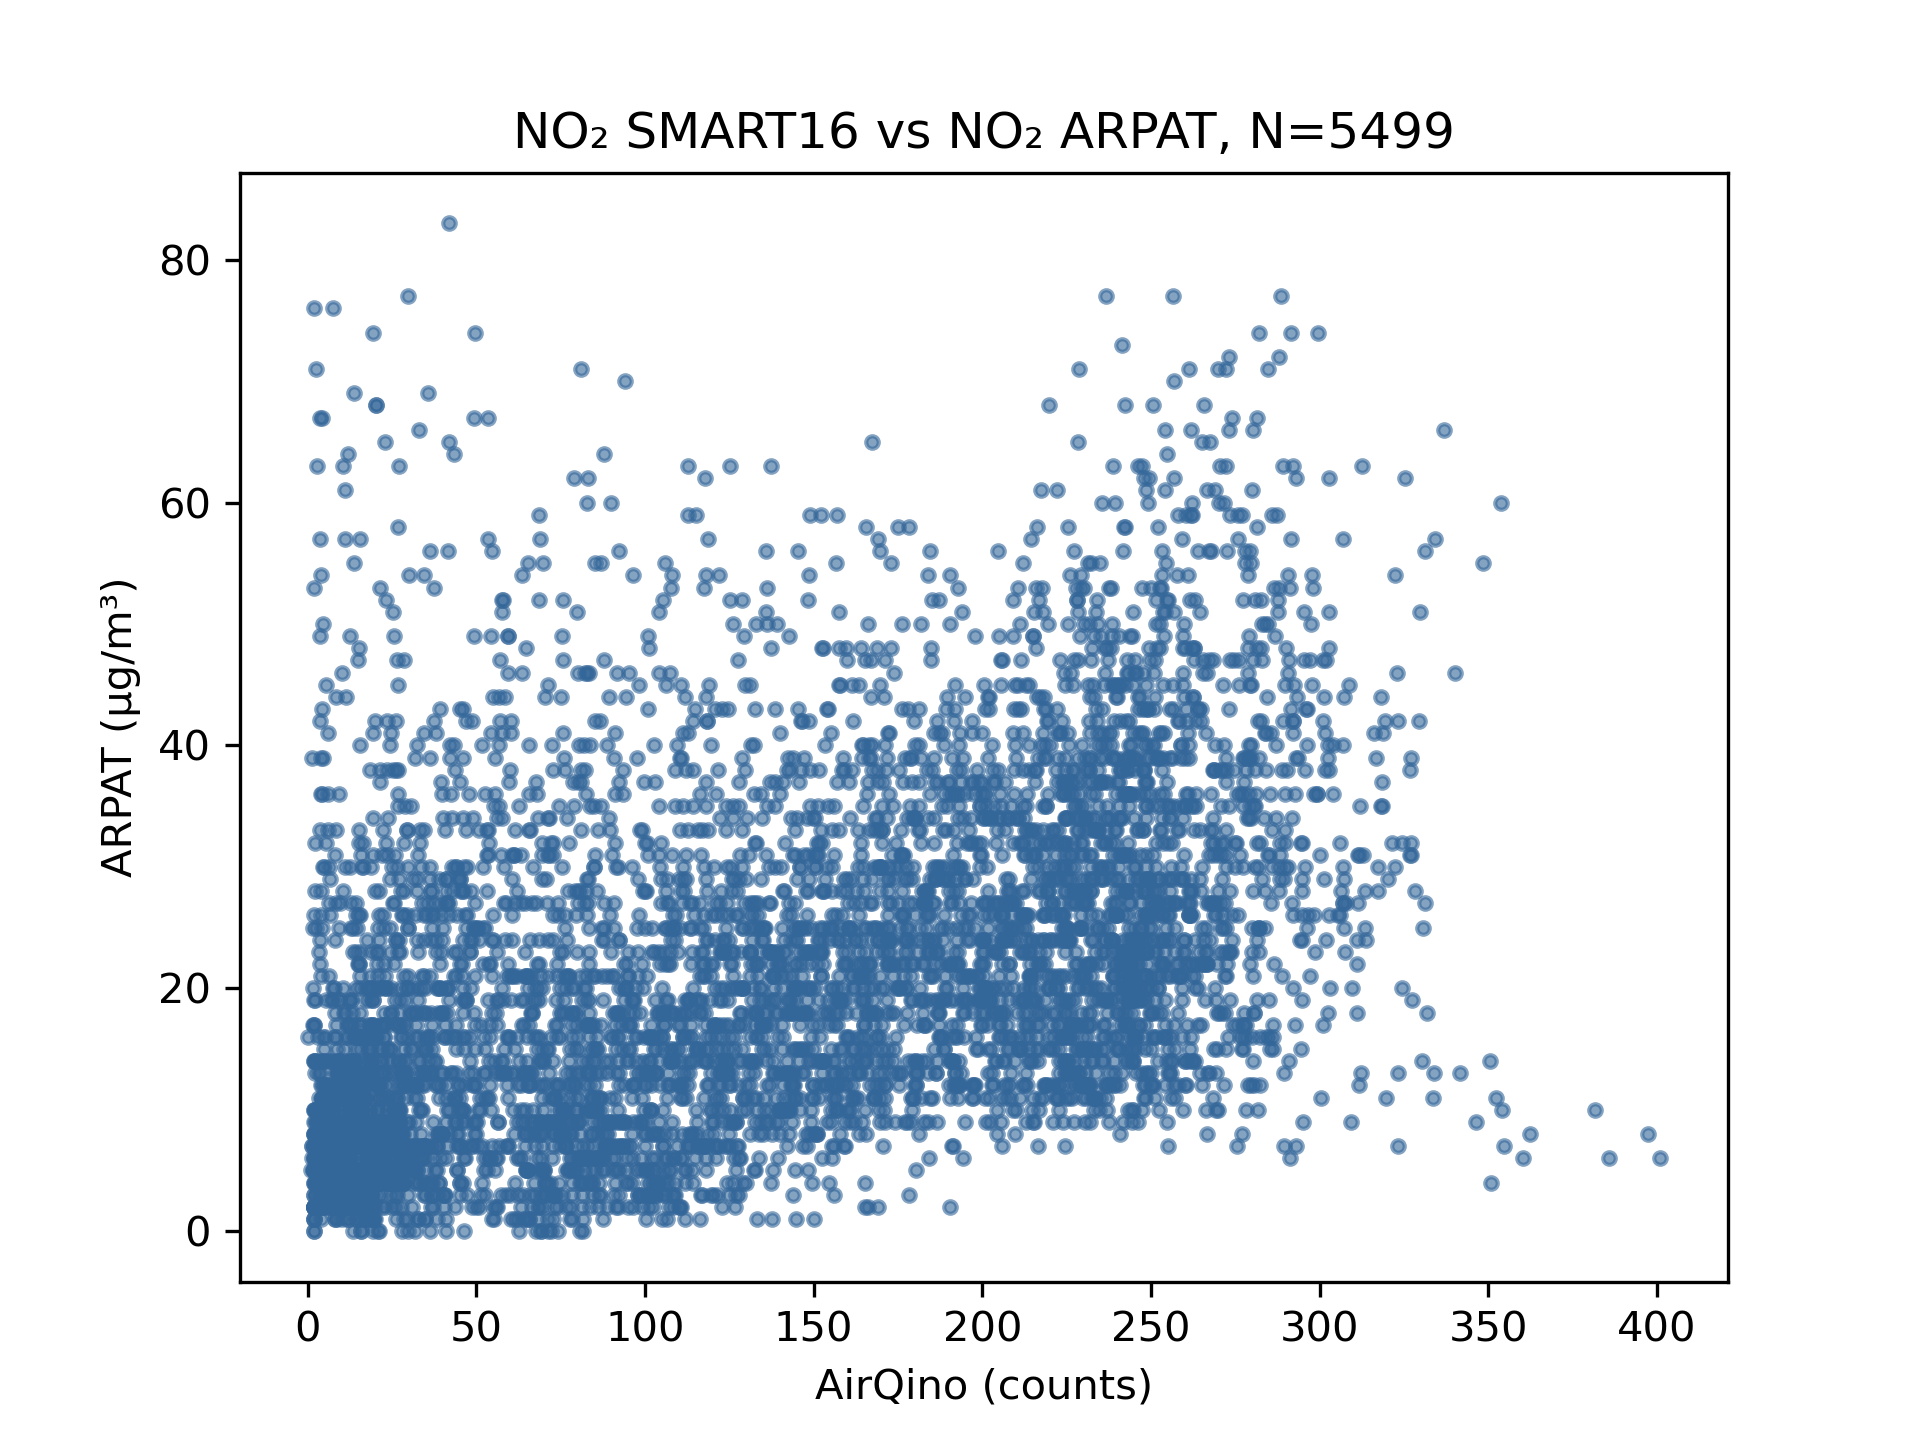
\includegraphics[width=0.55\textwidth,height=\textheight,keepaspectratio]{img/sc_no2.png}
\caption{Scatterplot dataset \ce{NO2}}
\label{fig:scatterplot_no2}
\end{figure}

I risultati dell'analisi grafica dei residui sono riportati in figura \ref{fig:residui_no2}.

\begin{figure}[H]
\centering
\subfloat[Scatterplot]{%
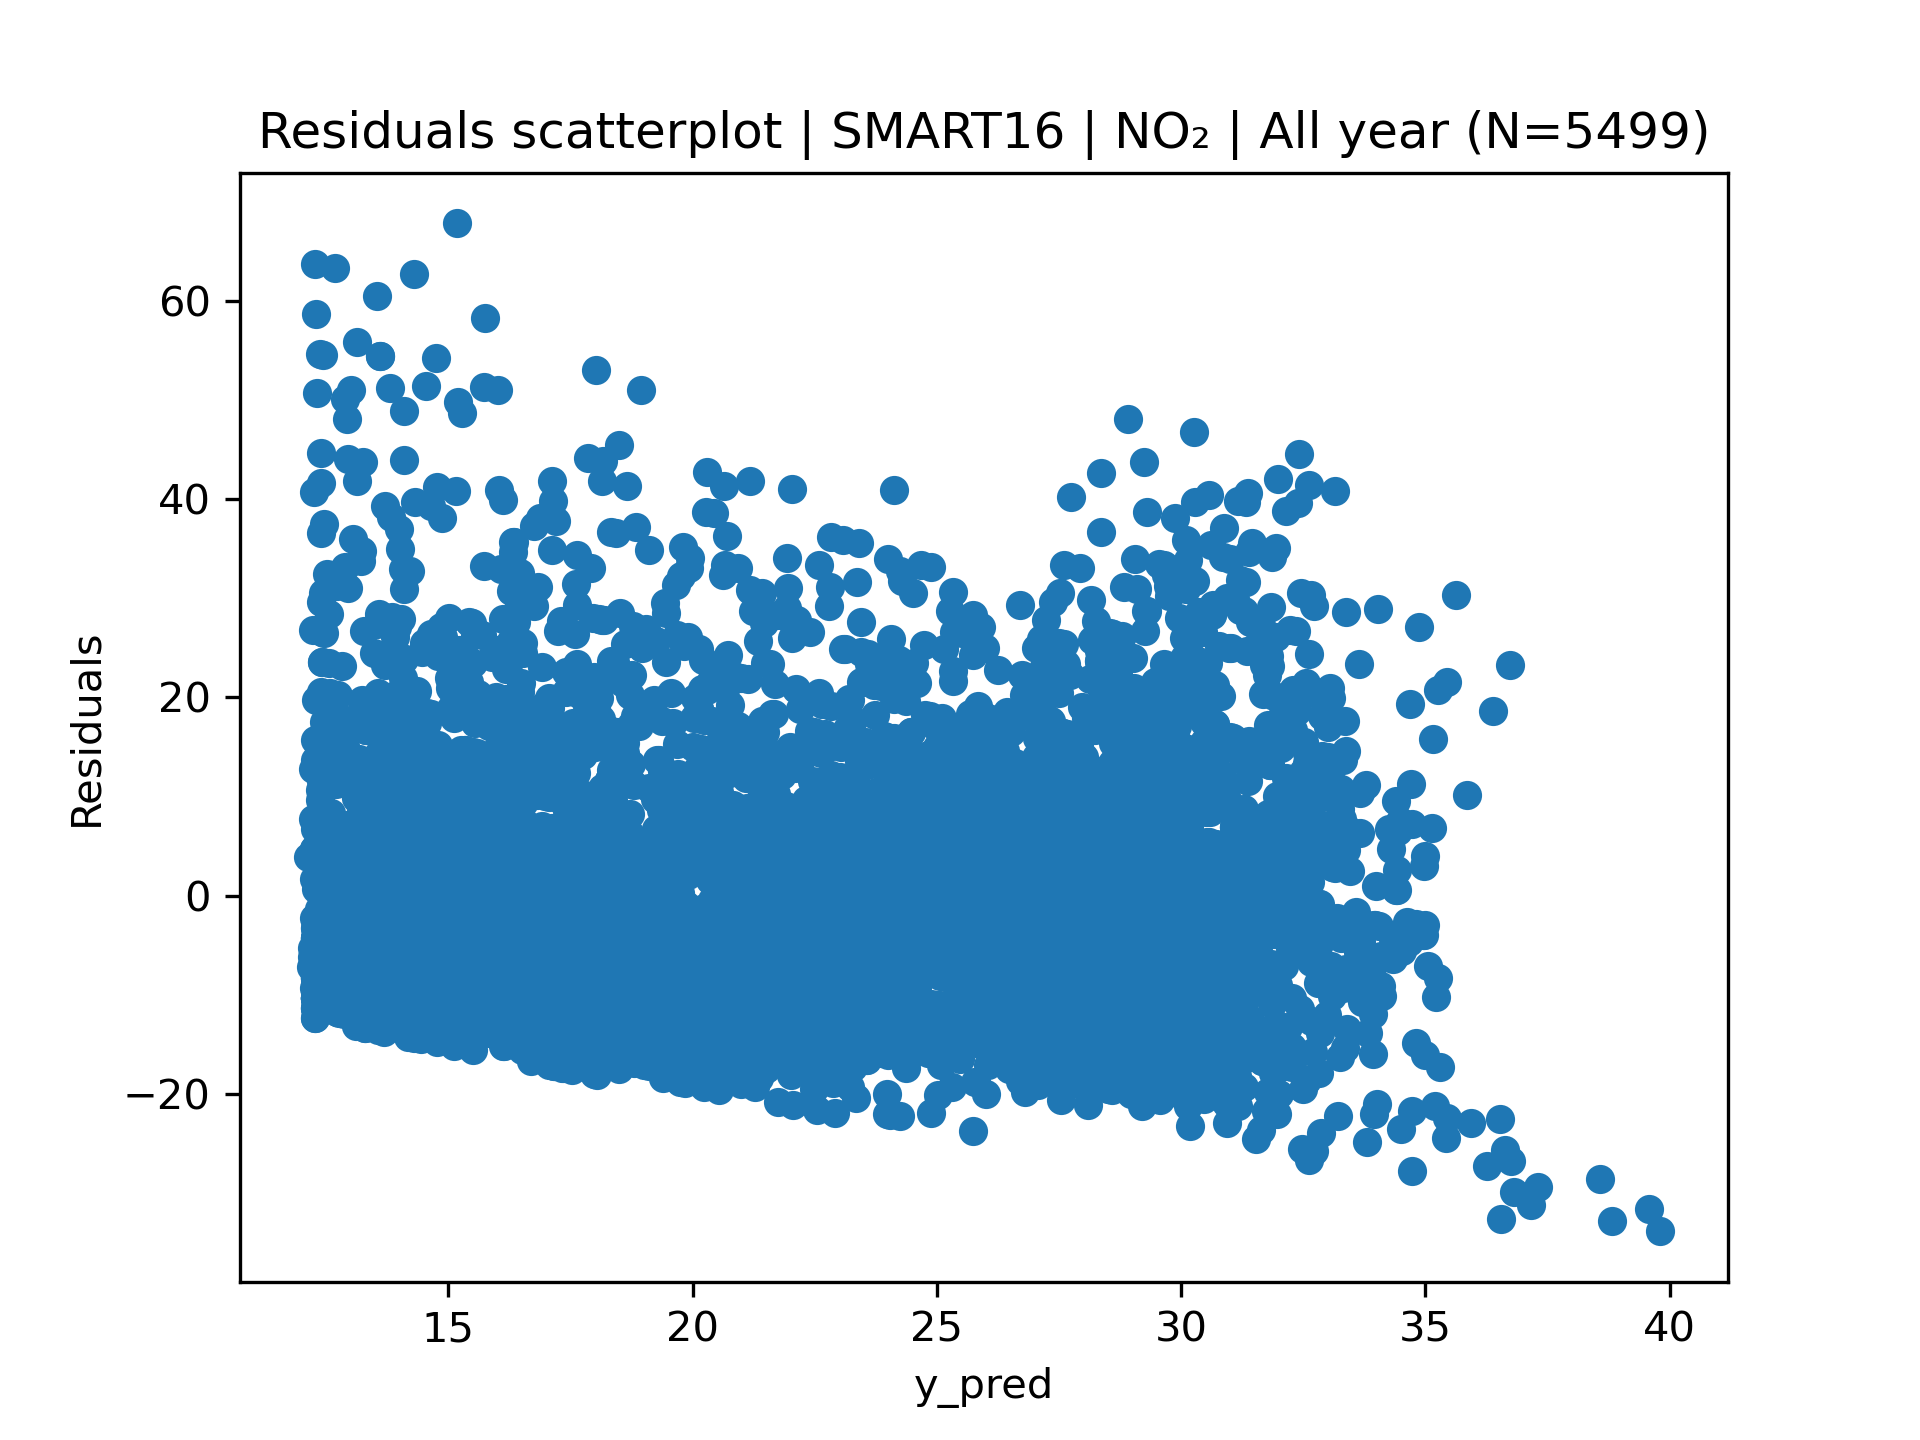
\includegraphics[width=0.42\textwidth]{img/res_no2_scatter}%
}\hfil
\subfloat[Plot]{%
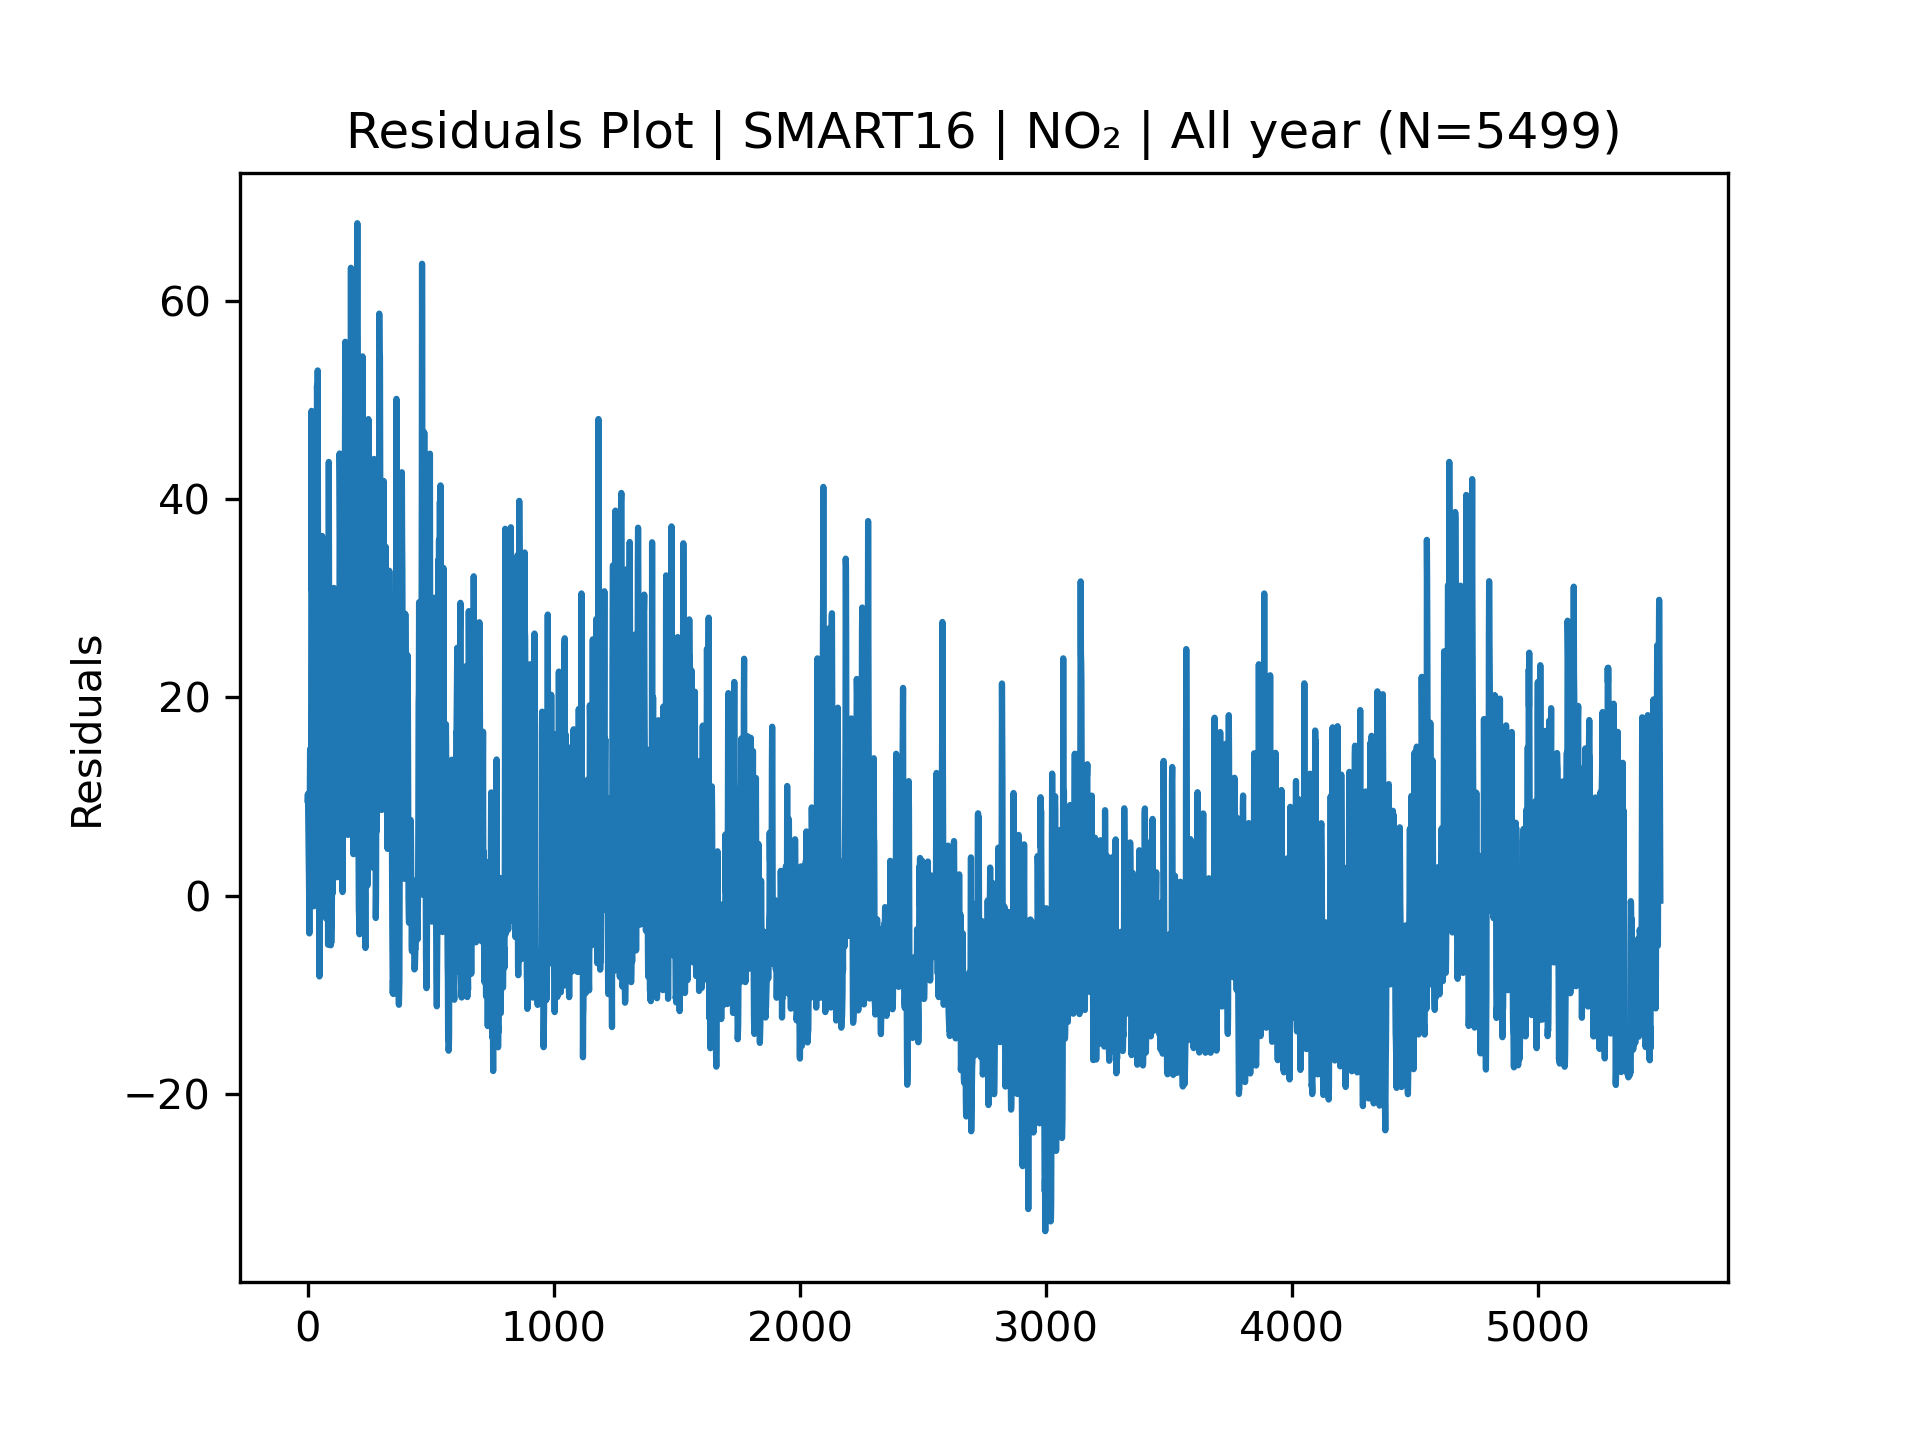
\includegraphics[width=0.42\textwidth]{img/res_no2_plot}%
}

\subfloat[Distribuzione]{%
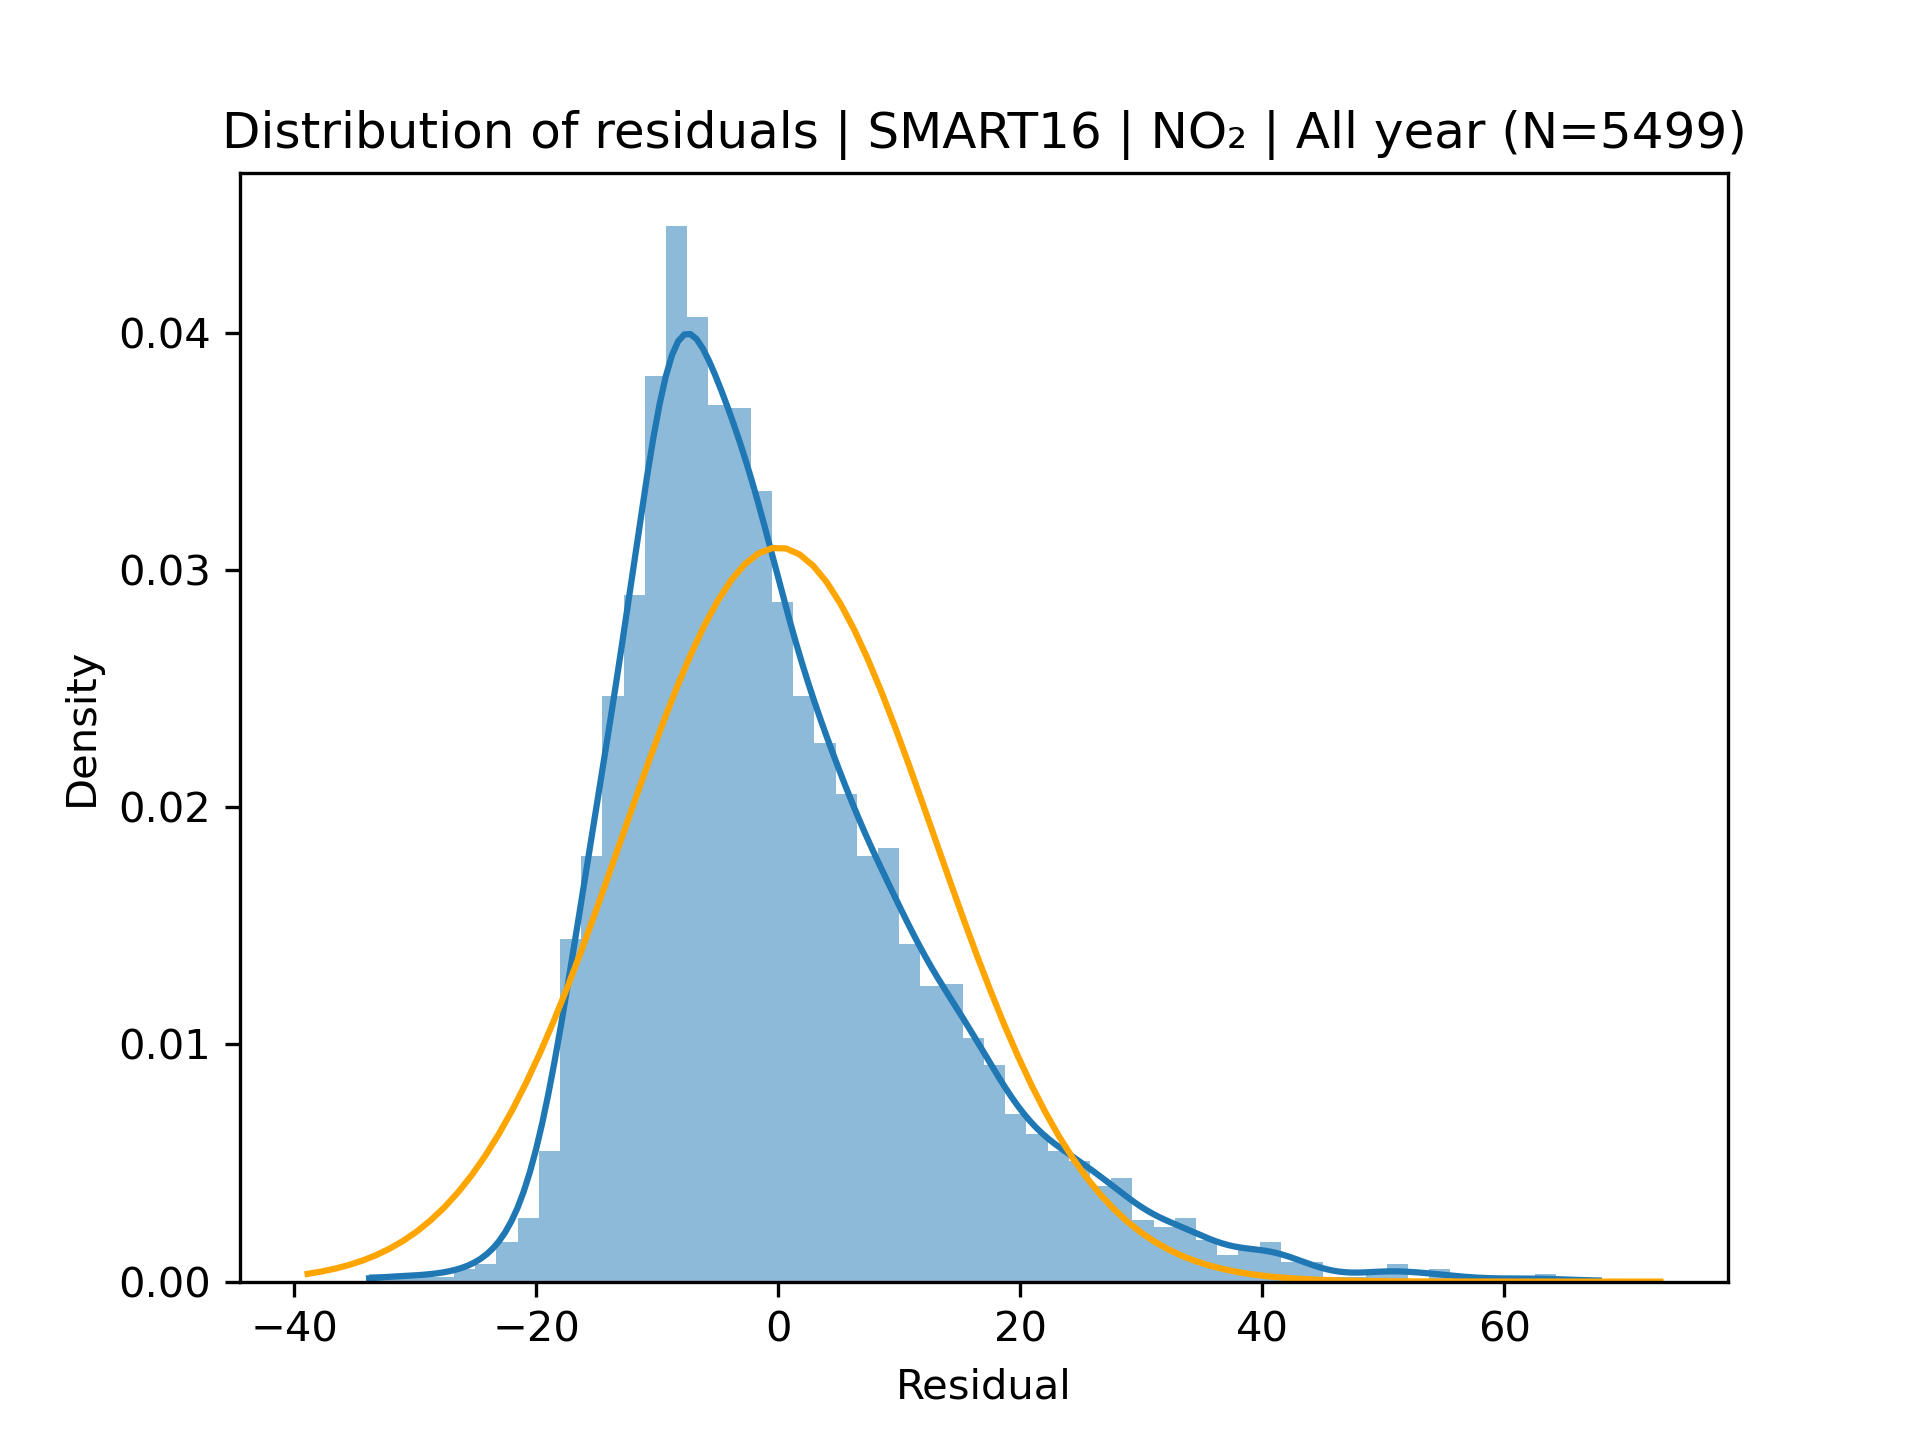
\includegraphics[width=0.42\textwidth]{img/res_no2_distr}%
}\hfil
\subfloat[Q-Q plot]{%
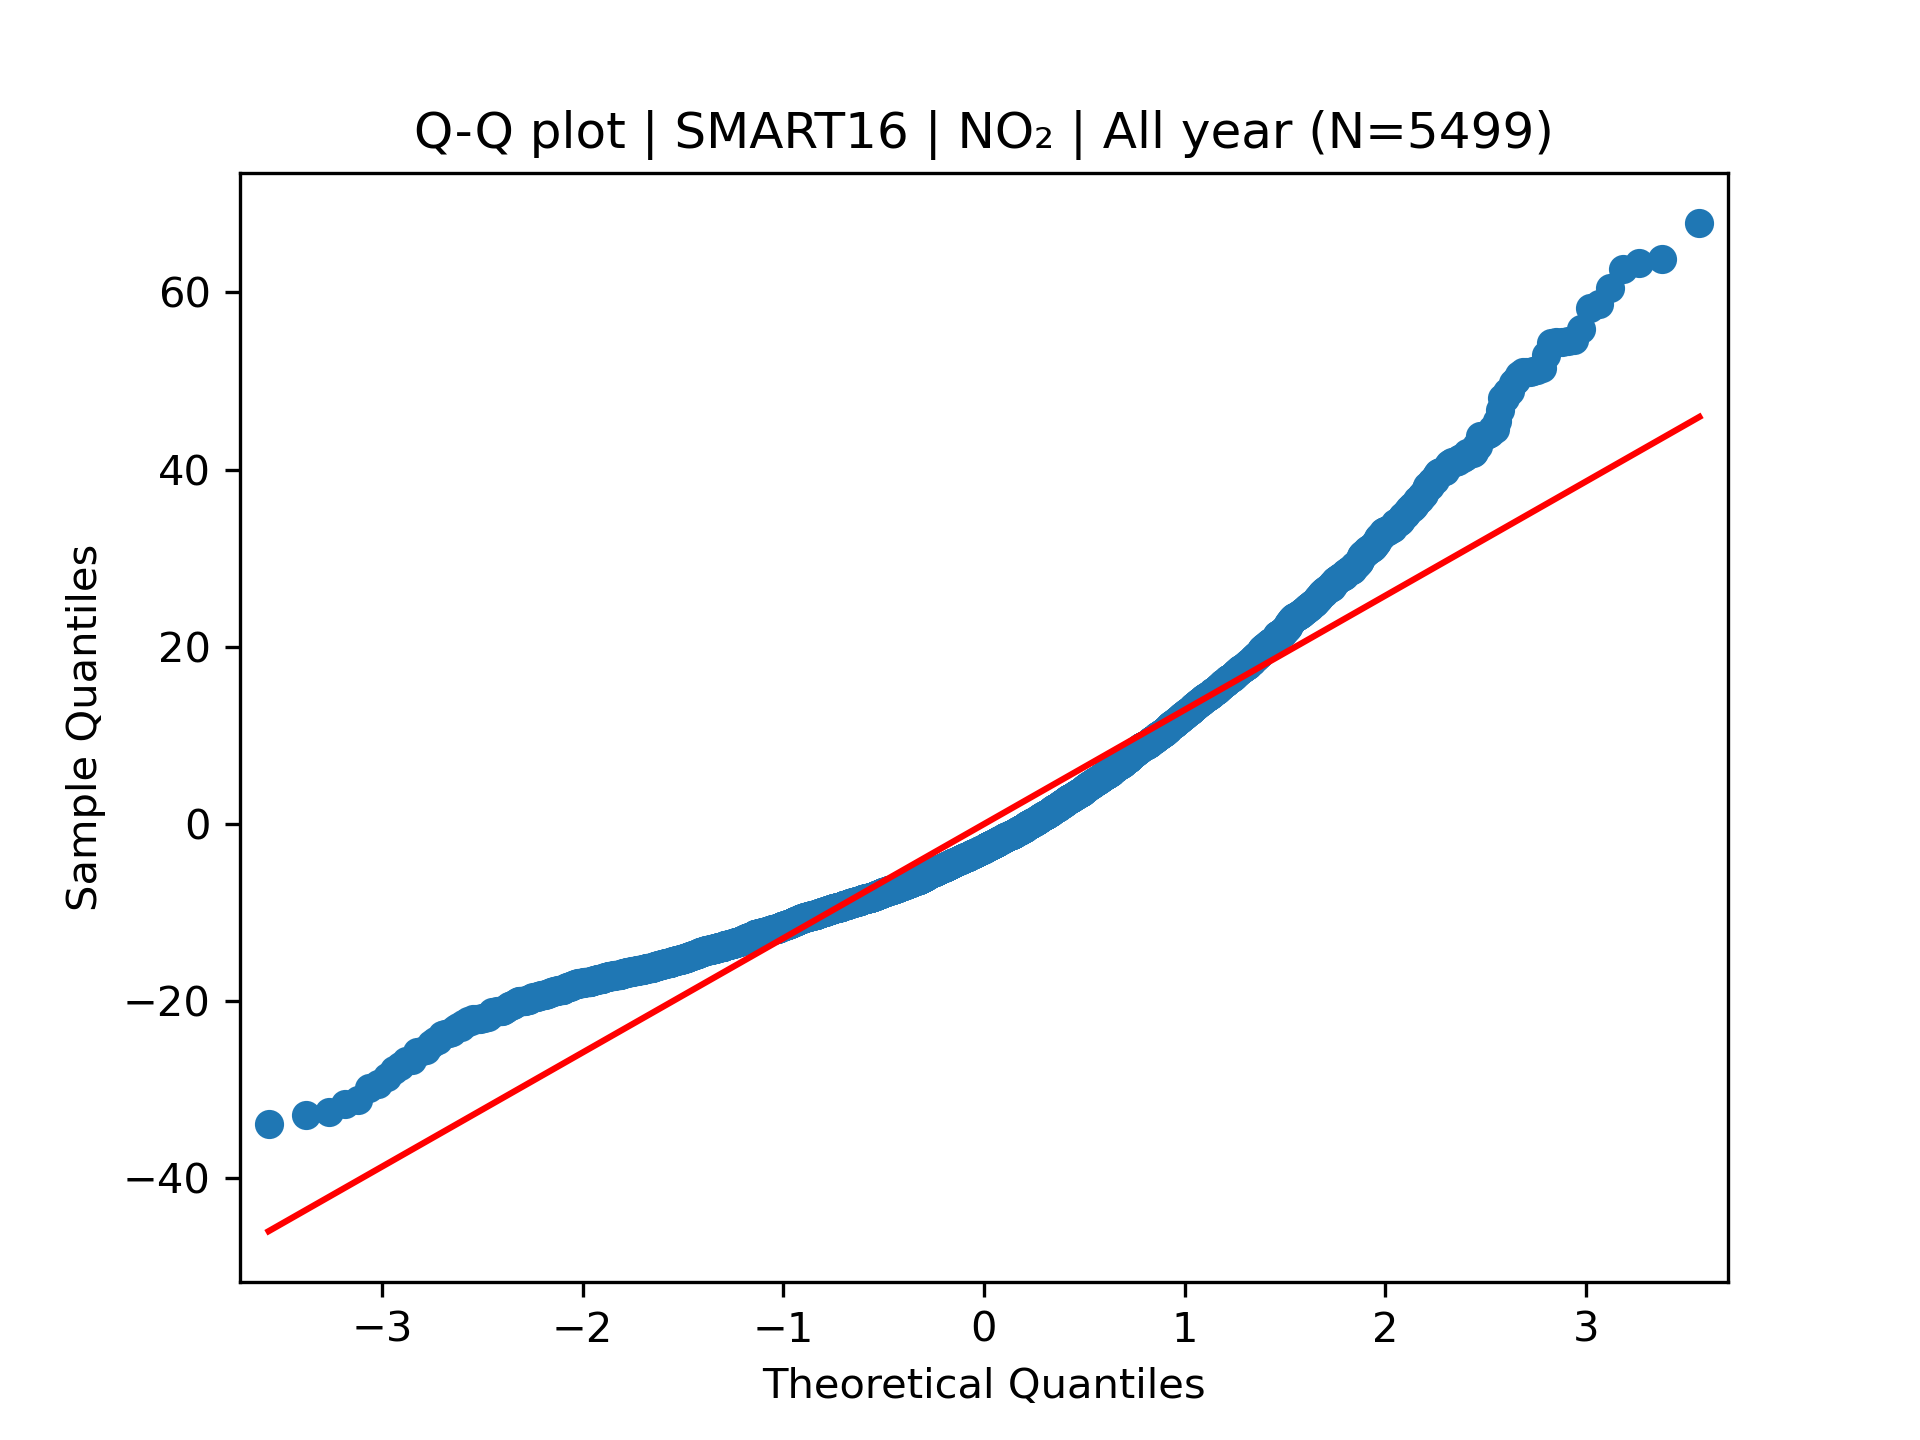
\includegraphics[width=0.42\textwidth]{img/res_no2_qq}%
}
\caption{Analisi dei residui dataset \ce{NO2}}
\label{fig:residui_no2}
\end{figure}

La tabella \ref{fig:risultati-no2} mostra i risultati, in termini di $R^2$ e RMSE, della procedura di calibrazione applicata al sensore di \ce{NO2} per ciascun modello di regressione, su tutto il dataset.

\begin{table}[H]
    \footnotesize
    \centering
    \def\arraystretch{0.9}
    \begin{tabular}{|l|c|c|}
    \hline
        \textbf{Modello di regressione} & $\bm{\mathrm{R^2}}$ & \textbf{RMSE (}$\mathrm{\si{\micro}g/m^3}$) \\ \hline
        Lineare & 0.304 & 11.393 \\ \hline
        Lineare robusto (Huber) & 0.312 & 11.424 \\ \hline
        \textbf{Lineare avanzato (Cook)} & \textbf{0.373} & \textbf{9.447} \\ \hline
        Ridge & 0.305 & 11.375 \\ \hline
        Lasso & 0.303 & 11.403 \\ \hline
        Polinomiale (grado 2) & 0.305 & 11.382 \\ \hline
        Polinomiale (grado 3) & 0.302 & 11.381 \\ \hline
        Random Forest & -0.034 & 13.839 \\ \hline
        Gradient Boosting & 0.103 & 12.887 \\ \hline
        SVR (Kernel lineare) & 0.287 & 11.528 \\ \hline
        SVR (Kernel polinomiale) & 0.255 & 11.816 \\ \hline
        SVR (Kernel RBF) & 0.294 & 11.445 \\ \hline
        KernelRidge & 0.301 & 11.344 \\ \hline
    \end{tabular}
    \caption{Risultati della calibrazione \ce{NO2}}
    \label{fig:risultati-no2}
\end{table}

E in figura \ref{fig:risultati-no2-hist} gli stessi risultati in forma di istogramma:

\begin{figure}[H]%
    \centering
    \captionsetup{justification=centering}
    \subfloat[\centering Risultati $\mathrm{R^2}$]{{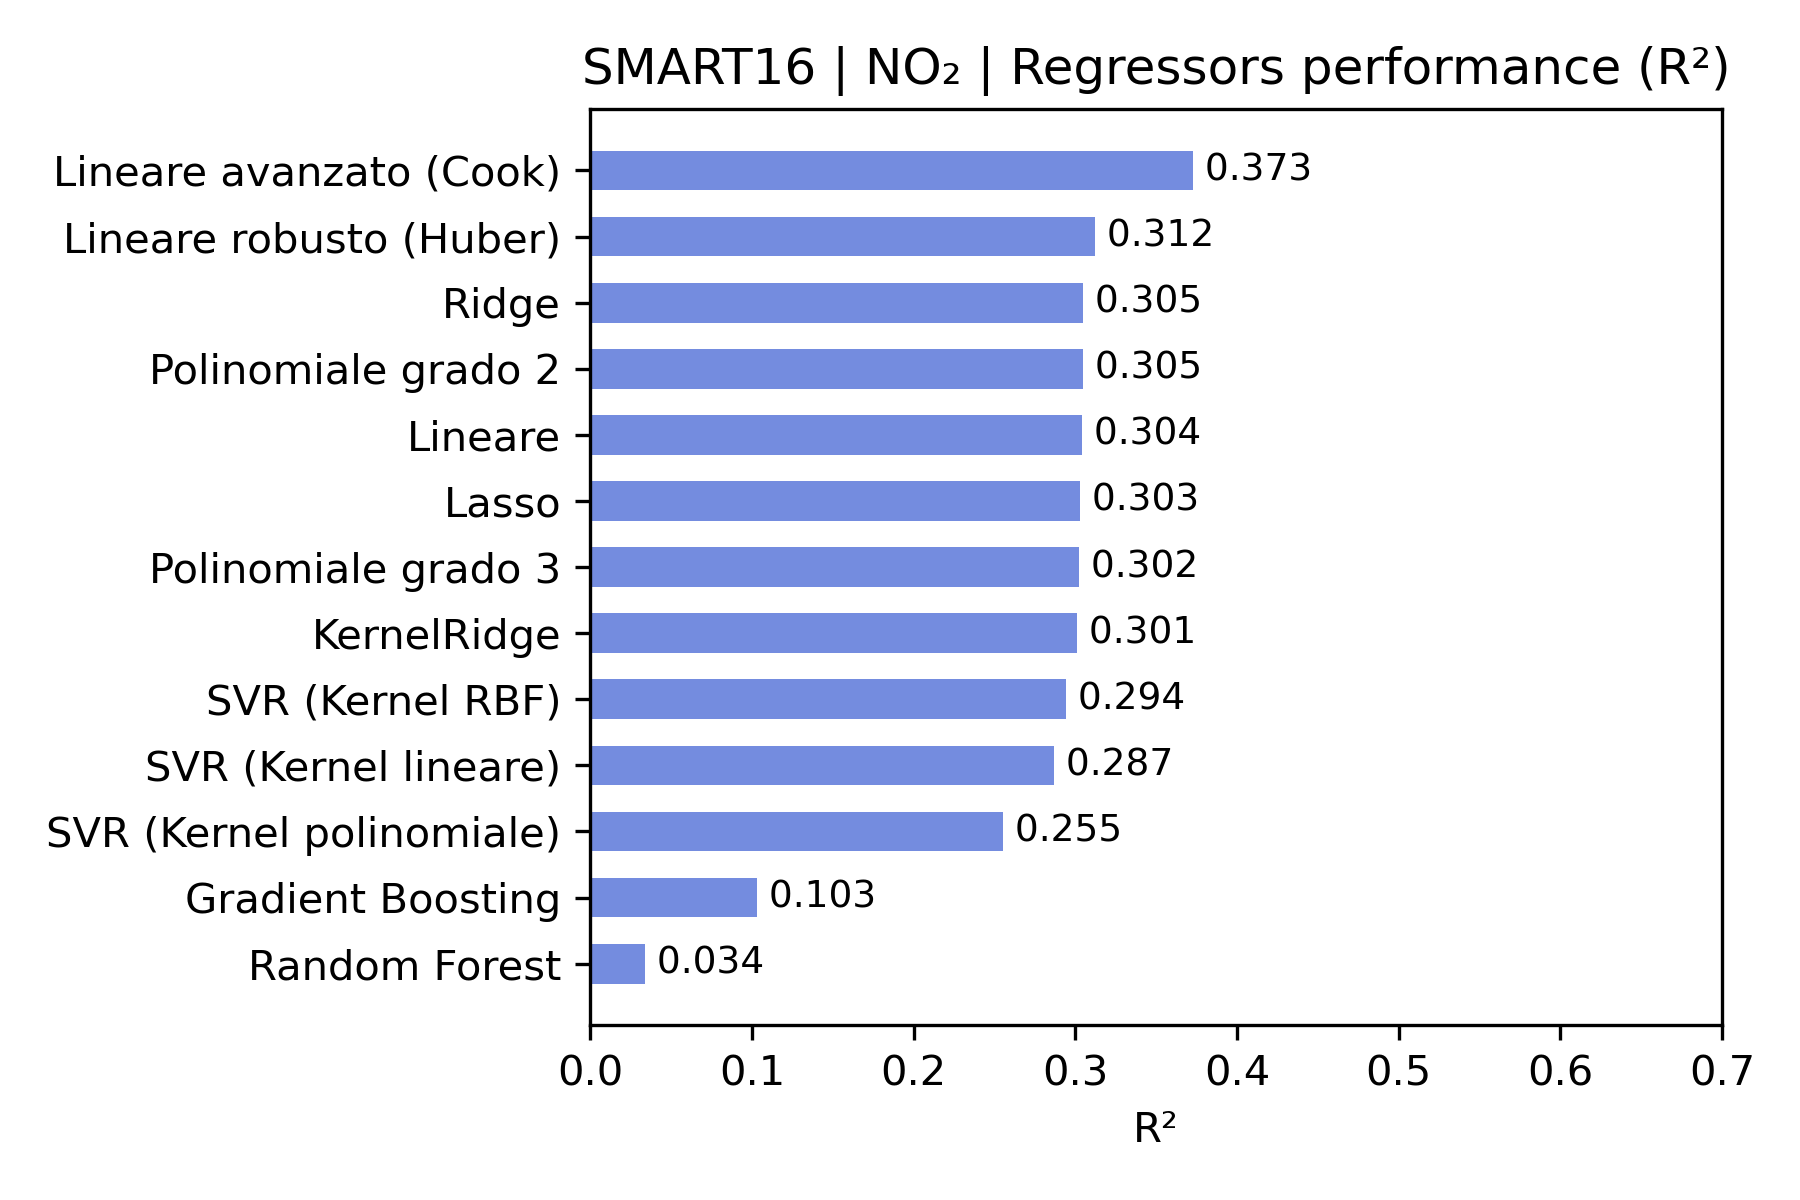
\includegraphics[width=6.9cm]{img/hist_no2_1} }}%
    \subfloat[\centering Risultati RMSE]{{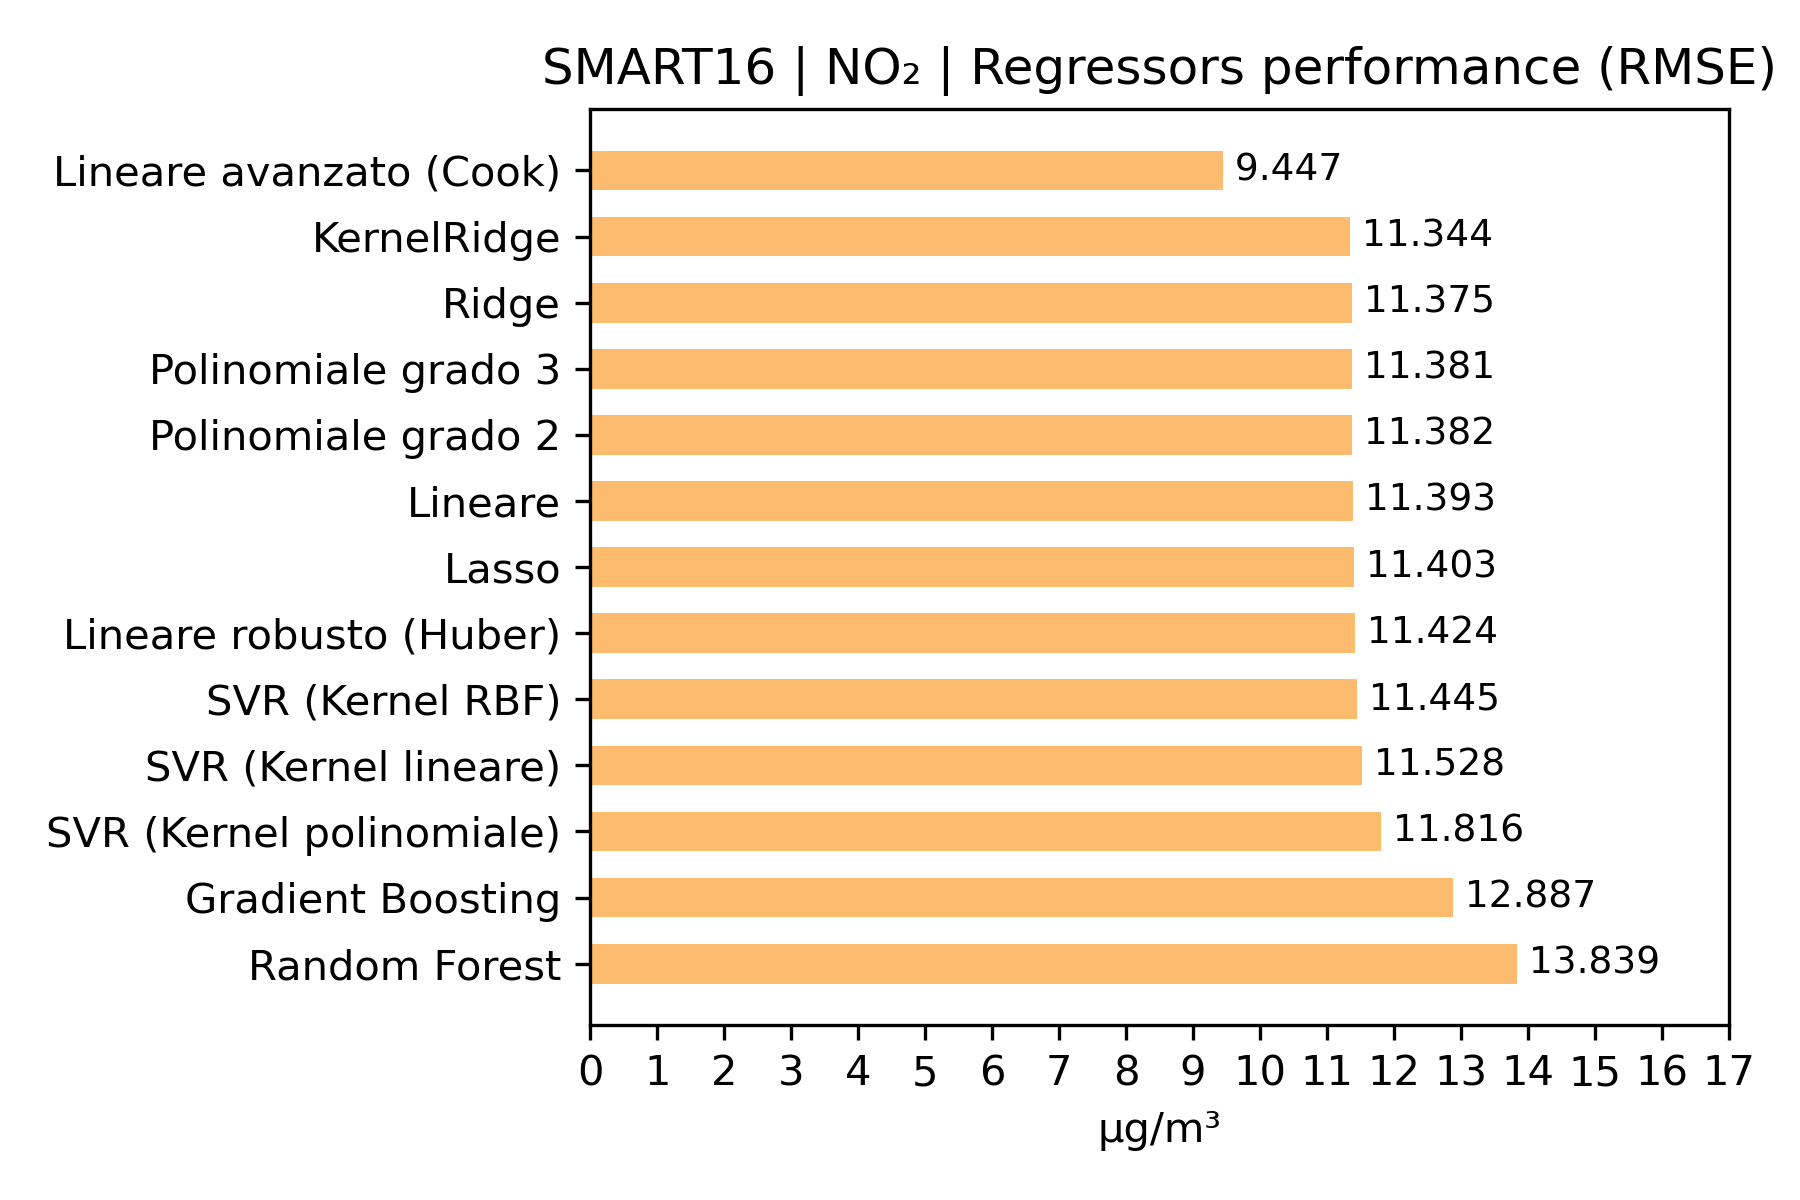
\includegraphics[width=6.9cm]{img/hist_no2_2} }}%
    \caption{Istogramma dei risultati della calibrazione \ce{NO2}}%
    \label{fig:risultati-no2-hist}%
\end{figure}

Per quanto riguarda l'applicazione del modello lineare \textit{avanzato}, è stata riapplicata la regressione dopo aver tolto tutti i punti con distanza di Cook (\ref{sssec:regressione-cook}) sopra una certa soglia ($\frac{4}{numero\ di\ osservazioni} = \frac{4}{5110} \approx 0,0007$). In particolare sono stati individuati e rimossi 282 outlier su 5110 osservazioni totali, circa il 5.52\% (figura \ref{fig:cook-no2}).

\begin{figure}[H]
\centering
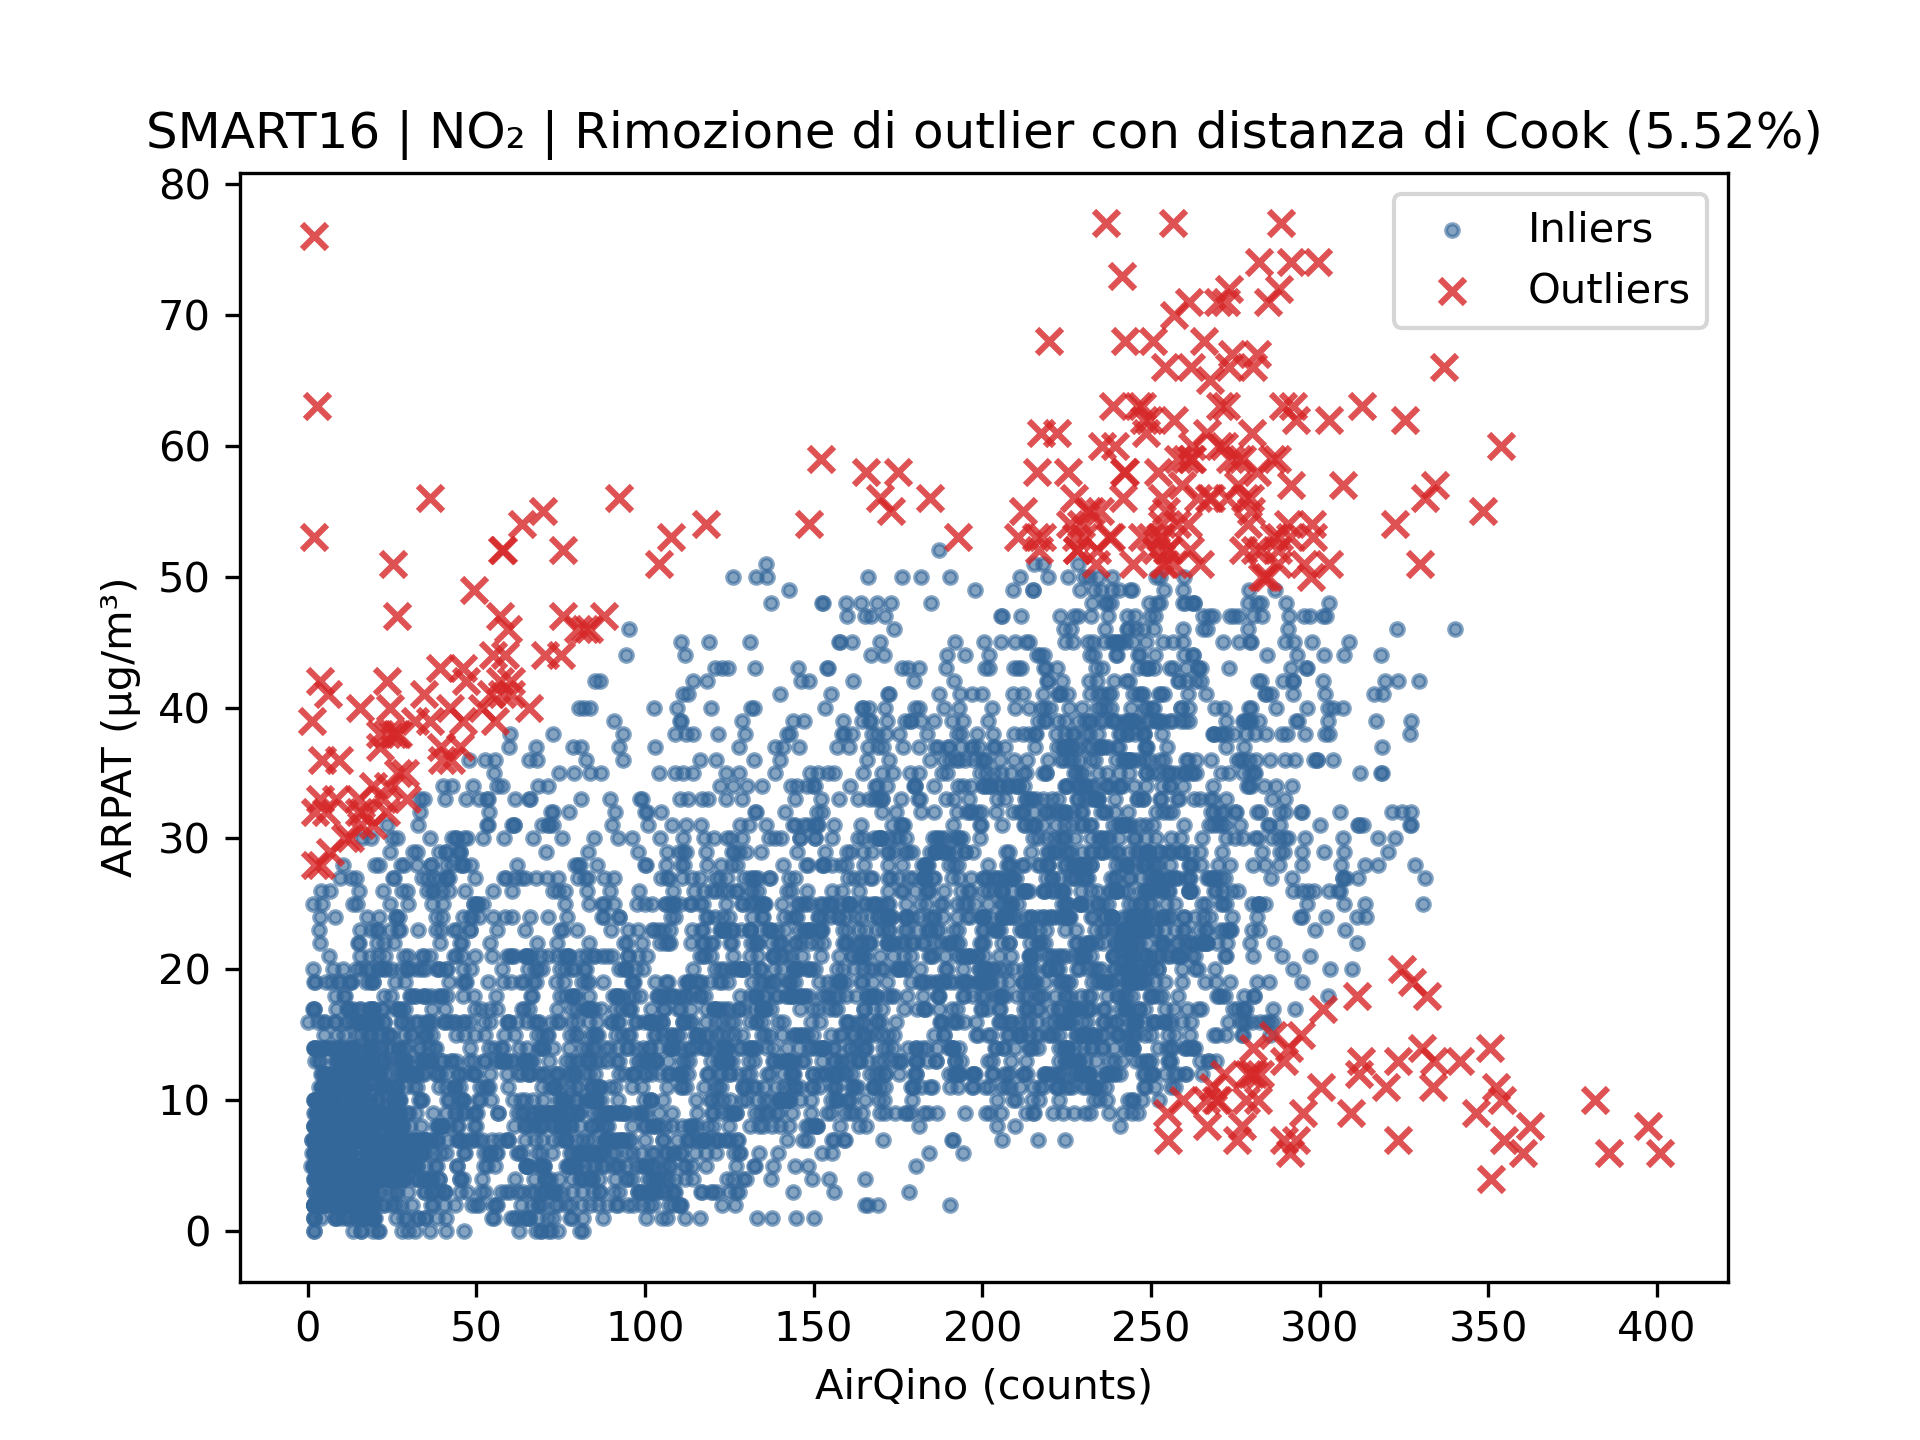
\includegraphics[width=0.75\textwidth,height=\textheight,keepaspectratio]{img/cook_no2.png}
\caption{Rimozione di outlier con distanza di Cook su dataset \ce{NO2}}%
\label{fig:cook-no2}%
\end{figure}

Nelle tabelle \ref{fig:risultati-no2-mese} e \ref{fig:risultati-no2-rmse-mese} sono invece riportati rispettivamente $R^2$ e RMSE della calibrazione su dataset \ce{NO2} fatta mese per mese.\\

Anche in questo caso il modello di regressione migliore è risultato in media quello \textit{avanzato}, con riconoscimento e rimozione di outlier, anche se per alcuni mesi il modello polinomiale di terzo grado e il modello KernelRidge hanno ottenuto risultati migliori.

\begin{table}[H]
    \footnotesize
    \centering
    \def\arraystretch{0.95}
    \begin{tabular}{|l|c|c|c|c|c|c|c|c|c|c|c|c|}
    \hline
        \textbf{Modello} & \textbf{Gen} & \textbf{Feb} & \textbf{Mar} & \textbf{Apr} & \textbf{Set} & \textbf{Ott} & \textbf{Nov} & \textbf{Dic} \\ \hline
        Lineare & 0.44 & 0.45 & 0.35 & 0.21 & 0.16 & 0.36 & 0.16 & 0.42 \\ \hline
        Lineare robusto (Huber) & 0.44 & 0.45 & 0.35 & 0.21 & 0.16 & 0.36 & 0.16 & 0.42 \\ \hline
        \textbf{Lineare avanzato (Cook)} & \textbf{0.53} & 0.48 & 0.38 & \textbf{0.27} & \textbf{0.29} & 0.39 & \textbf{0.18} & \textbf{0.45} \\ \hline
        Ridge & 0.45 & 0.45 & 0.35 & 0.20 & 0.17 & 0.37 & 0.16 & 0.43 \\ \hline
        Lasso & 0.43 & 0.45 & 0.34 & 0.21 & 0.16 & 0.37 & 0.17 & 0.42 \\ \hline
        Polinomiale (grado 2) & 0.42 & 0.46 & 0.37 & 0.24 & 0.27 & 0.39 & 0.17 & 0.42 \\ \hline
        Polinomiale (grado 3) & 0.42 & \textbf{0.51} & \textbf{0.48} & 0.23 & 0.27 & \textbf{0.41} & 0.17 & 0.42 \\ \hline
        Random Forest & 0.15 & 0.33 & 0.21 & -0.14 & -0.07 & 0.12 & -0.16 & 0.12 \\ \hline
        Gradient Boosting & 0.13 & 0.17 & 0.16 & 0.08 & 0.09 & 0.13 & 0.06 & 0.14 \\ \hline
        SVR (lineare) & 0.42 & 0.43 & 0.32 & 0.18 & 0.14 & 0.37 & 0.14 & 0.42 \\ \hline
        SVR (polinomiale) & 0.37 & 0.37 & 0.22 & 0.05 & 0.07 & 0.29 & 0.13 & 0.39 \\ \hline
        SVR (RBF) & 0.38 & 0.50 & 0.46 & 0.19 & 0.25 & 0.39 & 0.14 & 0.43 \\ \hline
        KernelRidge & 0.44 & 0.45 & 0.37 & 0.24 & 0.26 & 0.39 & \textbf{0.18} & 0.41 \\ \hline
    \end{tabular}
    \caption{Risultati della calibrazione \ce{NO2} mese per mese ($R^2$)}
    \label{fig:risultati-no2-mese}
\end{table}

\begin{table}[H]
    \footnotesize
    \centering
    \def\arraystretch{0.95}
    \setlength{\tabcolsep}{5pt}
    \begin{tabular}{|l|c|c|c|c|c|c|c|c|c|c|c|c|}
    \hline
        \textbf{Modello} & \textbf{Gen} & \textbf{Feb} & \textbf{Mar} & \textbf{Apr} & \textbf{Set} & \textbf{Ott} & \textbf{Nov} & \textbf{Dic} \\ \hline
        Lineare & 13.31 & 11.68 & 9.90 & 9.30 & 8.73 & 8.72 & 12.30 & 9.86 \\ \hline
        Lineare robusto (Huber) & 13.27 & 11.55 & 9.91 & 9.34 & 8.70 & 8.75 & 12.36 & 9.80 \\ \hline
        \textbf{Lineare avanzato (Cook)} & \textbf{11.32} & \textbf{10.13} & \textbf{8.64} & \textbf{6.95} & \textbf{7.08} & \textbf{7.99} & \textbf{10.64} & \textbf{9.42} \\ \hline
        Ridge & 13.23 & 11.52 & 9.91 & 9.18 & 8.73 & 8.67 & 12.33 & 9.72 \\ \hline
        Lasso & 13.43 & 11.56 & 9.99 & 9.31 & 8.73 & 8.81 & 12.23 & 9.94 \\ \hline
        Polinomiale (grado 2) & 13.54 & 11.46 & 9.66 & 9.11 & 8.19 & 8.57 & 12.36 & 9.72 \\ \hline
        Polinomiale (grado 3) & 13.54 & 10.99 & 8.88 & 9.17 & 8.15 & 8.39 & 12.27 & 9.79 \\ \hline
        Random Forest & 16.27 & 12.76 & 10.85 & 11.11 & 9.84 & 10.27 & 14.58 & 12.03 \\ \hline
        Gradient Boosting & 16.64 & 14.30 & 11.30 & 9.90 & 9.09 & 10.34 & 13.04 & 11.98 \\ \hline
        SVR (lineare) & 13.51 & 11.82 & 10.21 & 9.53 & 8.82 & 8.77 & 12.35 & 9.86 \\ \hline
        SVR (polinomiale) & 14.10 & 12.43 & 10.74 & 10.07 & 9.29 & 9.23 & 12.51 & 10.05 \\ \hline
        SVR (RBF) & 13.70 & 10.98 & 9.02 & 9.39 & 8.24 & 8.57 & 12.50 & 9.74 \\ \hline
        KernelRidge & 13.35 & 11.51 & 9.80 & 9.17 & 8.21 & 8.62 & 12.06 & 9.78 \\ \hline
    \end{tabular}
    \caption{Risultati della calibrazione \ce{NO2} mese per mese (RMSE)}
    \label{fig:risultati-no2-rmse-mese}
\end{table}

Infine, la tabella \ref{fig:risultati-no2-coefficienti} riporta i coefficienti delle curve di regressione ottenuti applicando i modelli al dataset \ce{NO2}. I coefficienti \textit{a}, \textit{b}, \textit{c}, \textit{d}, \textit{e} si riferiscono ad una equazione polinomiale generica del tipo $y=a+bx+cx^2+dx^3+ex^4$.

\begin{table}[H]
    \footnotesize
    \centering
    \begin{tabular}{|l|c|c|c|c|c|c|c|}
    \hline
        \textbf{Modello di regressione} & \textbf{a} & \textbf{b} & \textbf{c} & \textbf{d} & \textbf{e} \\ \hline
        Lineare & 6.52 & 12.25 & / & / & / \\ \hline
        Lineare robusto (Huber) & 6.62 & 11.98 & / & / & / \\ \hline
        Lineare avanzato (Cook) & 6.84 & 9.56 & / & / & / \\ \hline
        Lasso & 6.52 & 12.26 & / & / & / \\ \hline
        Ridge & 6.52 & 12.25 & / & / & / \\ \hline
        Polinomiale (grado 2) & 12.11 & 6.83 & -0.10 & / & / \\ \hline
        Polinomiale (grado 3) & 12.71 & 4.23 & 1.91 & -0.40 & / \\ \hline
        Polinomiale (grado 4) & 9.97 & 22.86 & -22.40 & 10.21 & -1.47 \\ \hline
    \end{tabular}
    \caption{Coefficienti della calibrazione \ce{NO2}}
    \label{fig:risultati-no2-coefficienti}
\end{table}

\subsection{Risultati \ce{PM_{2.5}}}\label{ssec:risultati-pm2.5}

Il confronto tra le misurazioni AirQino e le misurazioni di riferimento ARPAT per \ce{PM_{2.5}} sono riportate nello \textit{scatterplot} di figura \ref{fig:scatterplot_pm2.5}.

\clearpage

\begin{figure}[H]
\centering
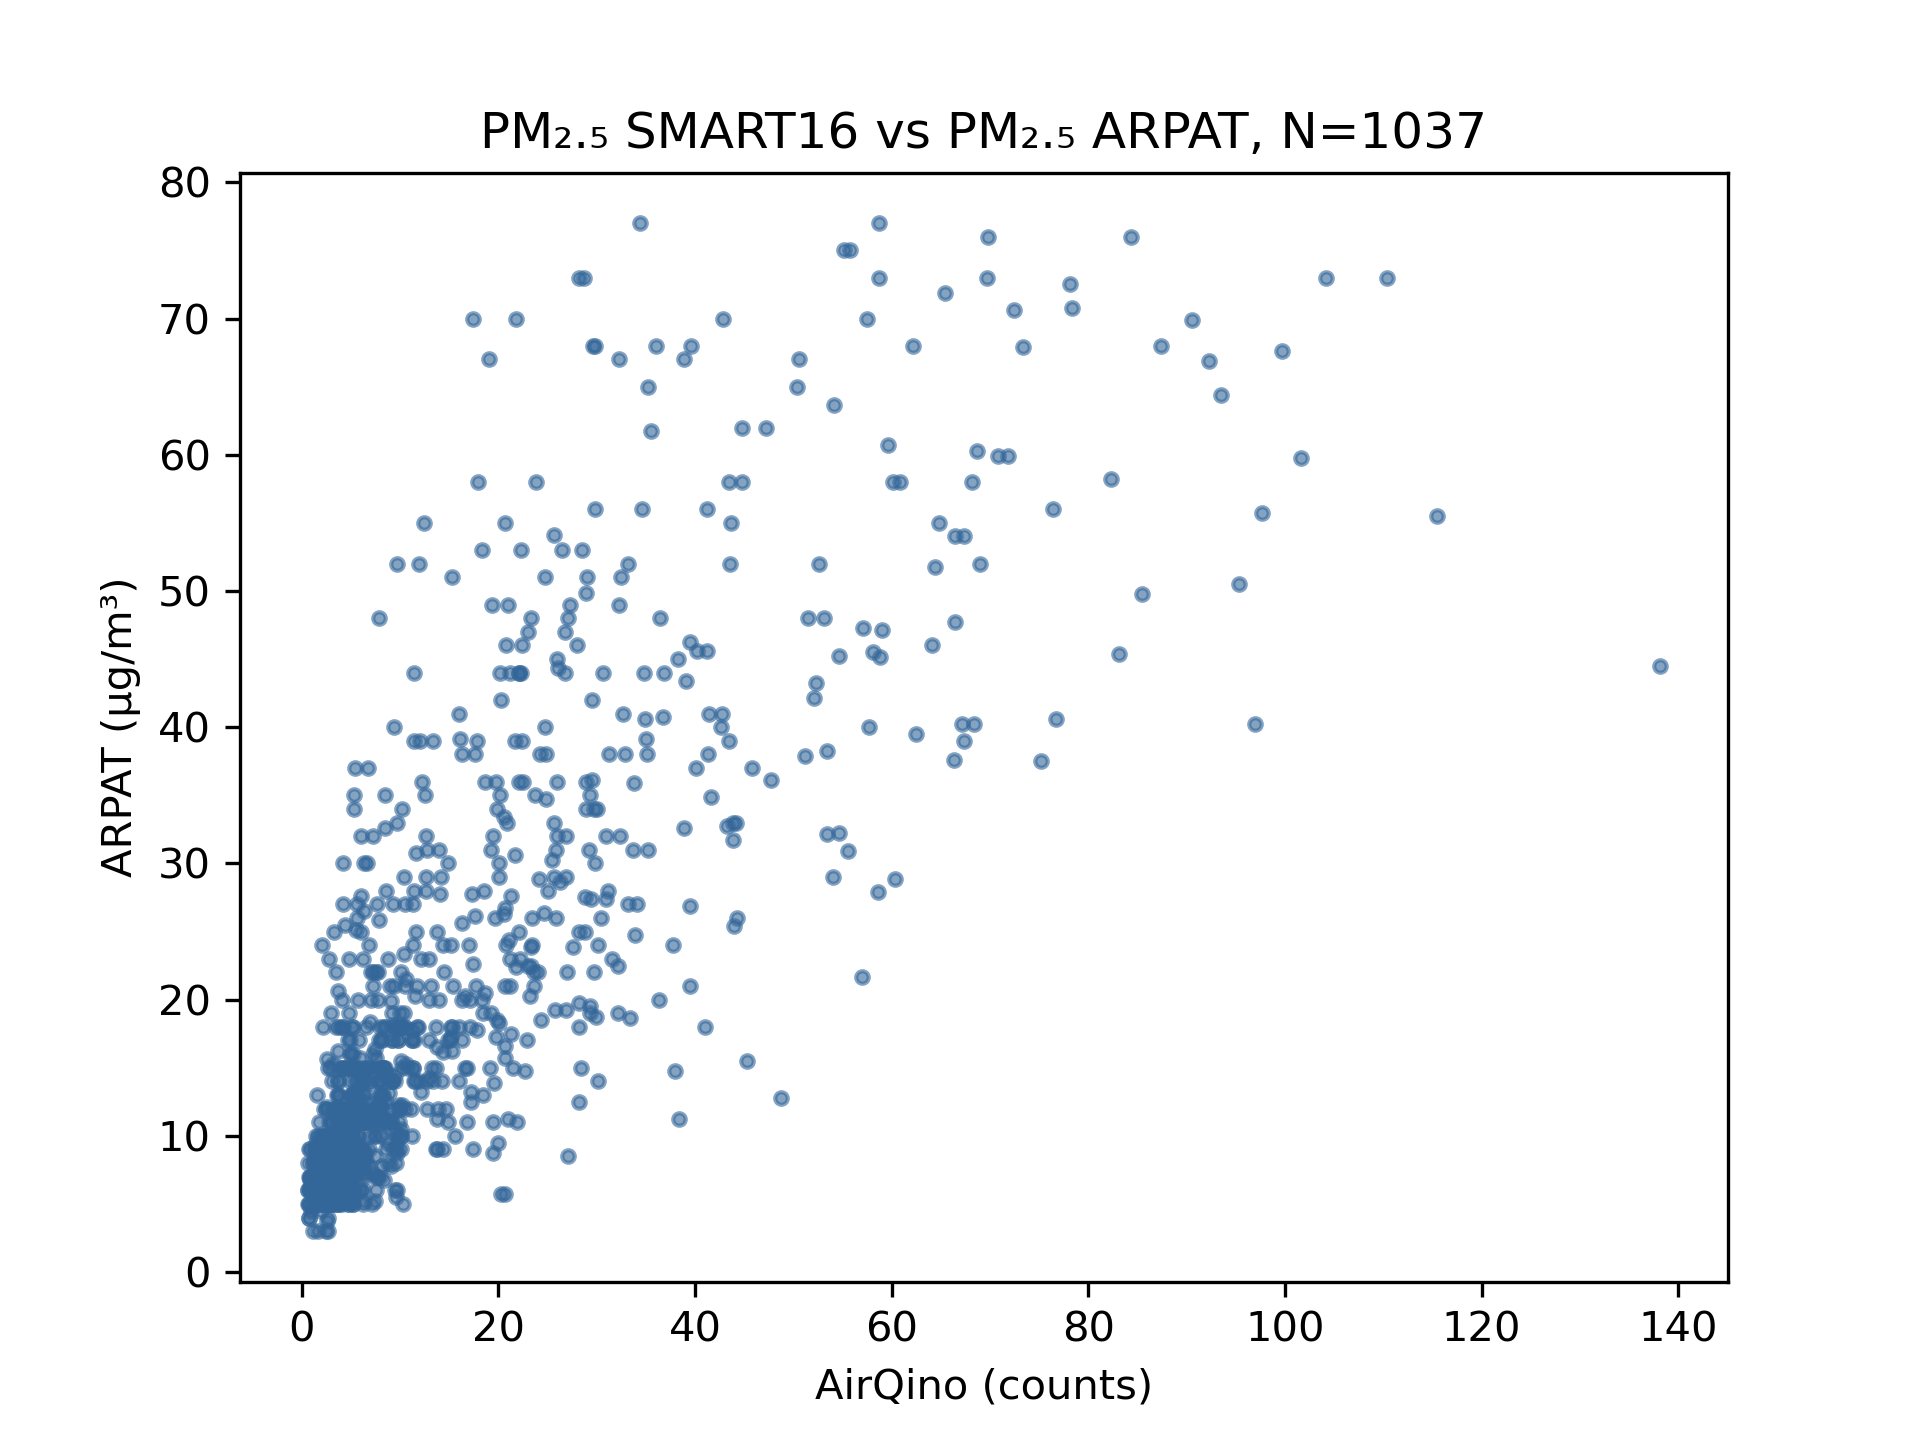
\includegraphics[width=0.55\textwidth,height=\textheight,keepaspectratio]{img/sc_pm2.5.png}
\caption{Scatterplot dataset \ce{PM_{2.5}}}
\label{fig:scatterplot_pm2.5}
\end{figure}

I risultati dell'analisi grafica dei residui sono riportati in figura \ref{fig:residui_pm2.5}.

\begin{figure}[H]
\centering
\subfloat[Scatterplot]{%
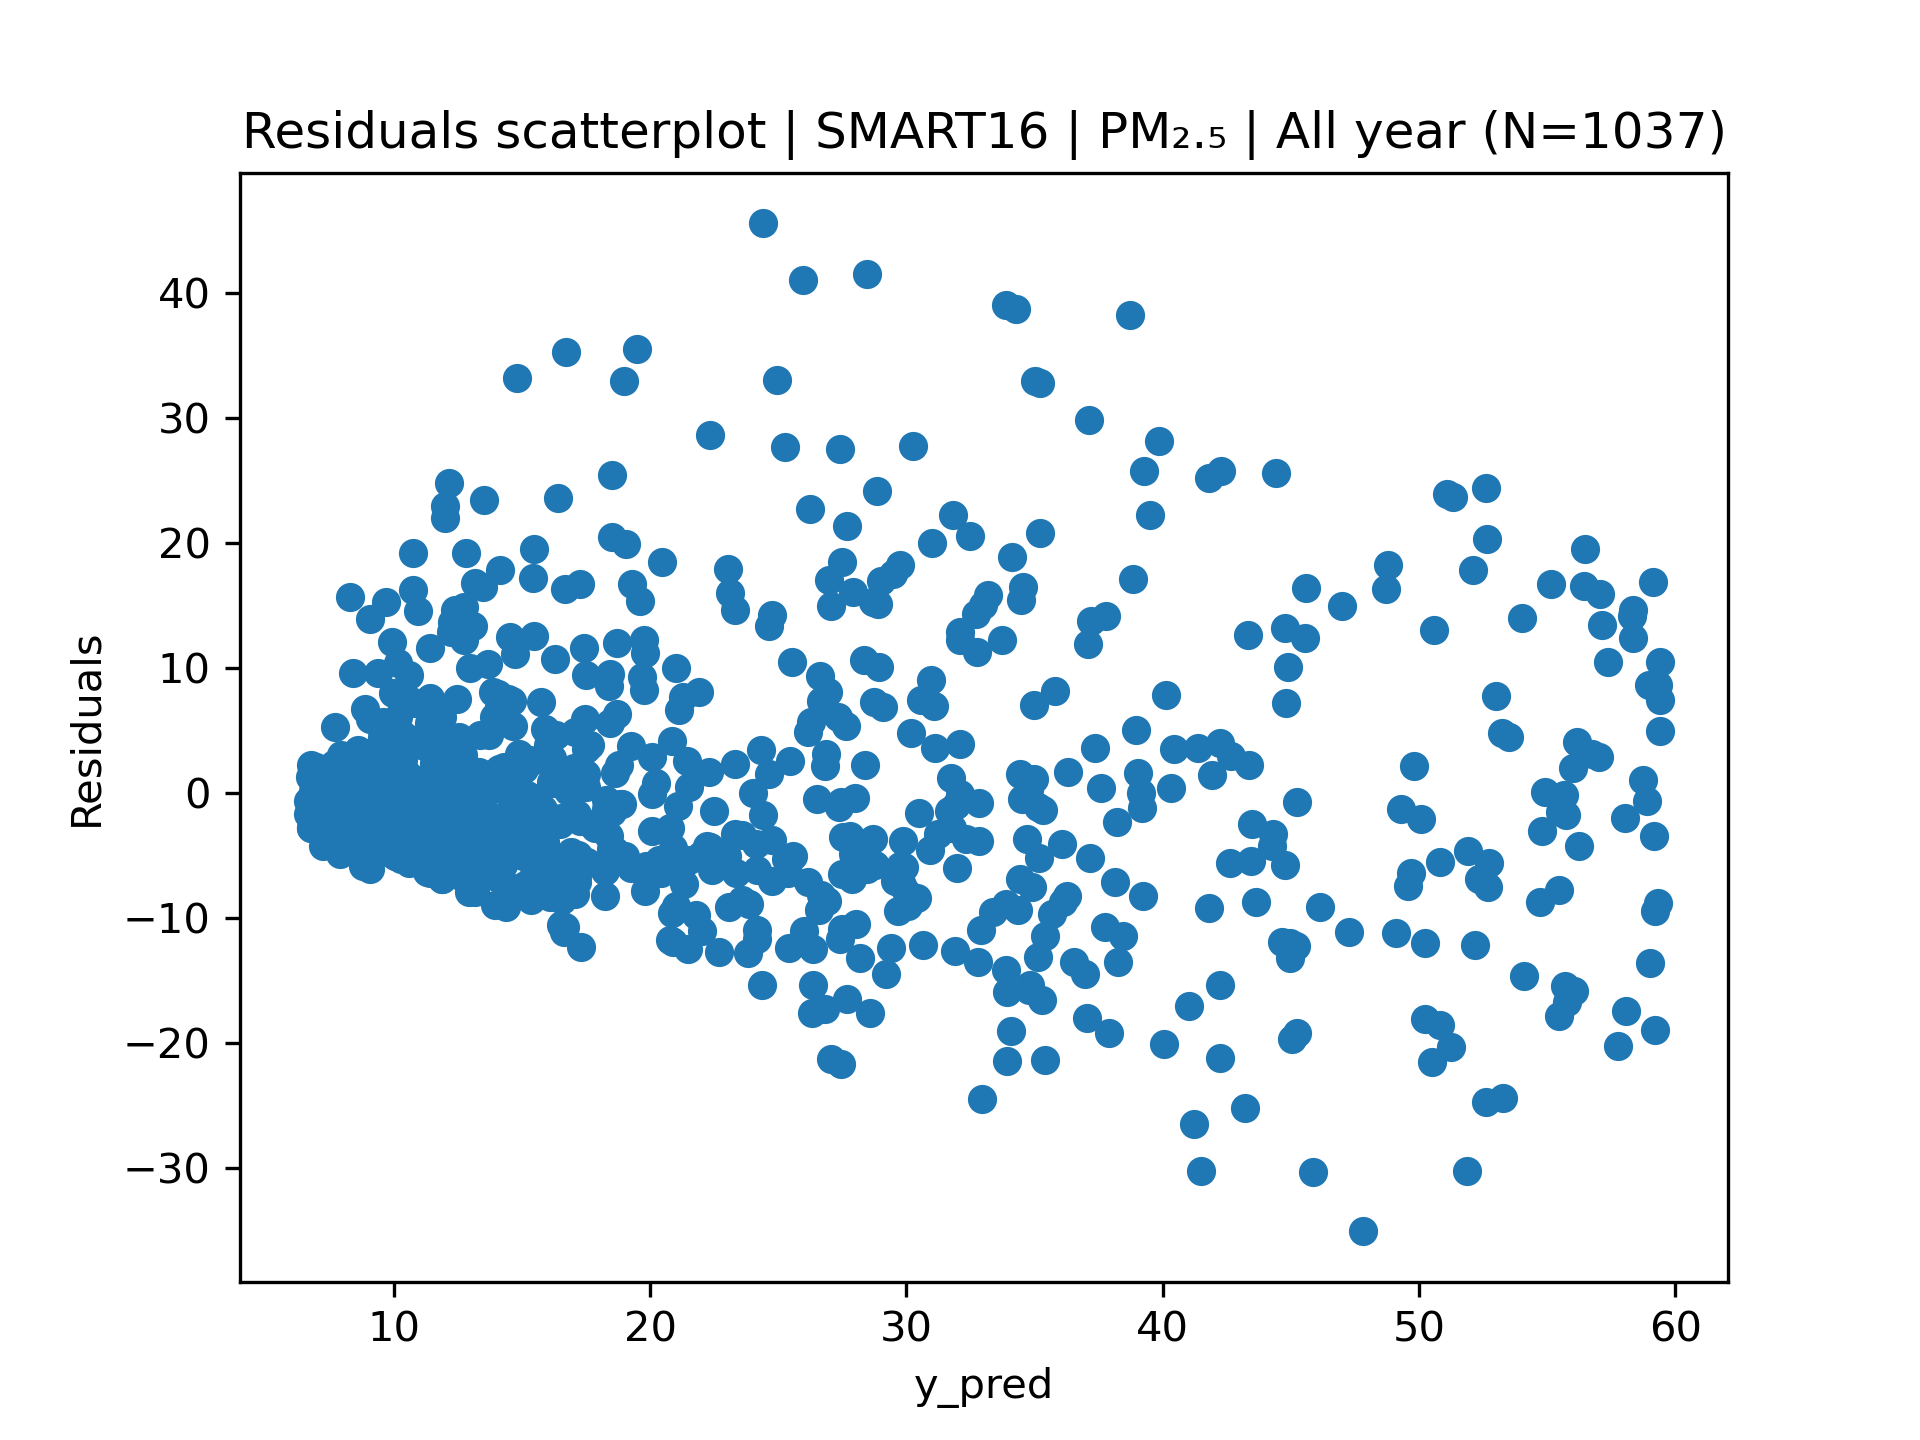
\includegraphics[width=0.42\textwidth]{img/res_pm2.5_scatter}%
}\hfil
\subfloat[Plot]{%
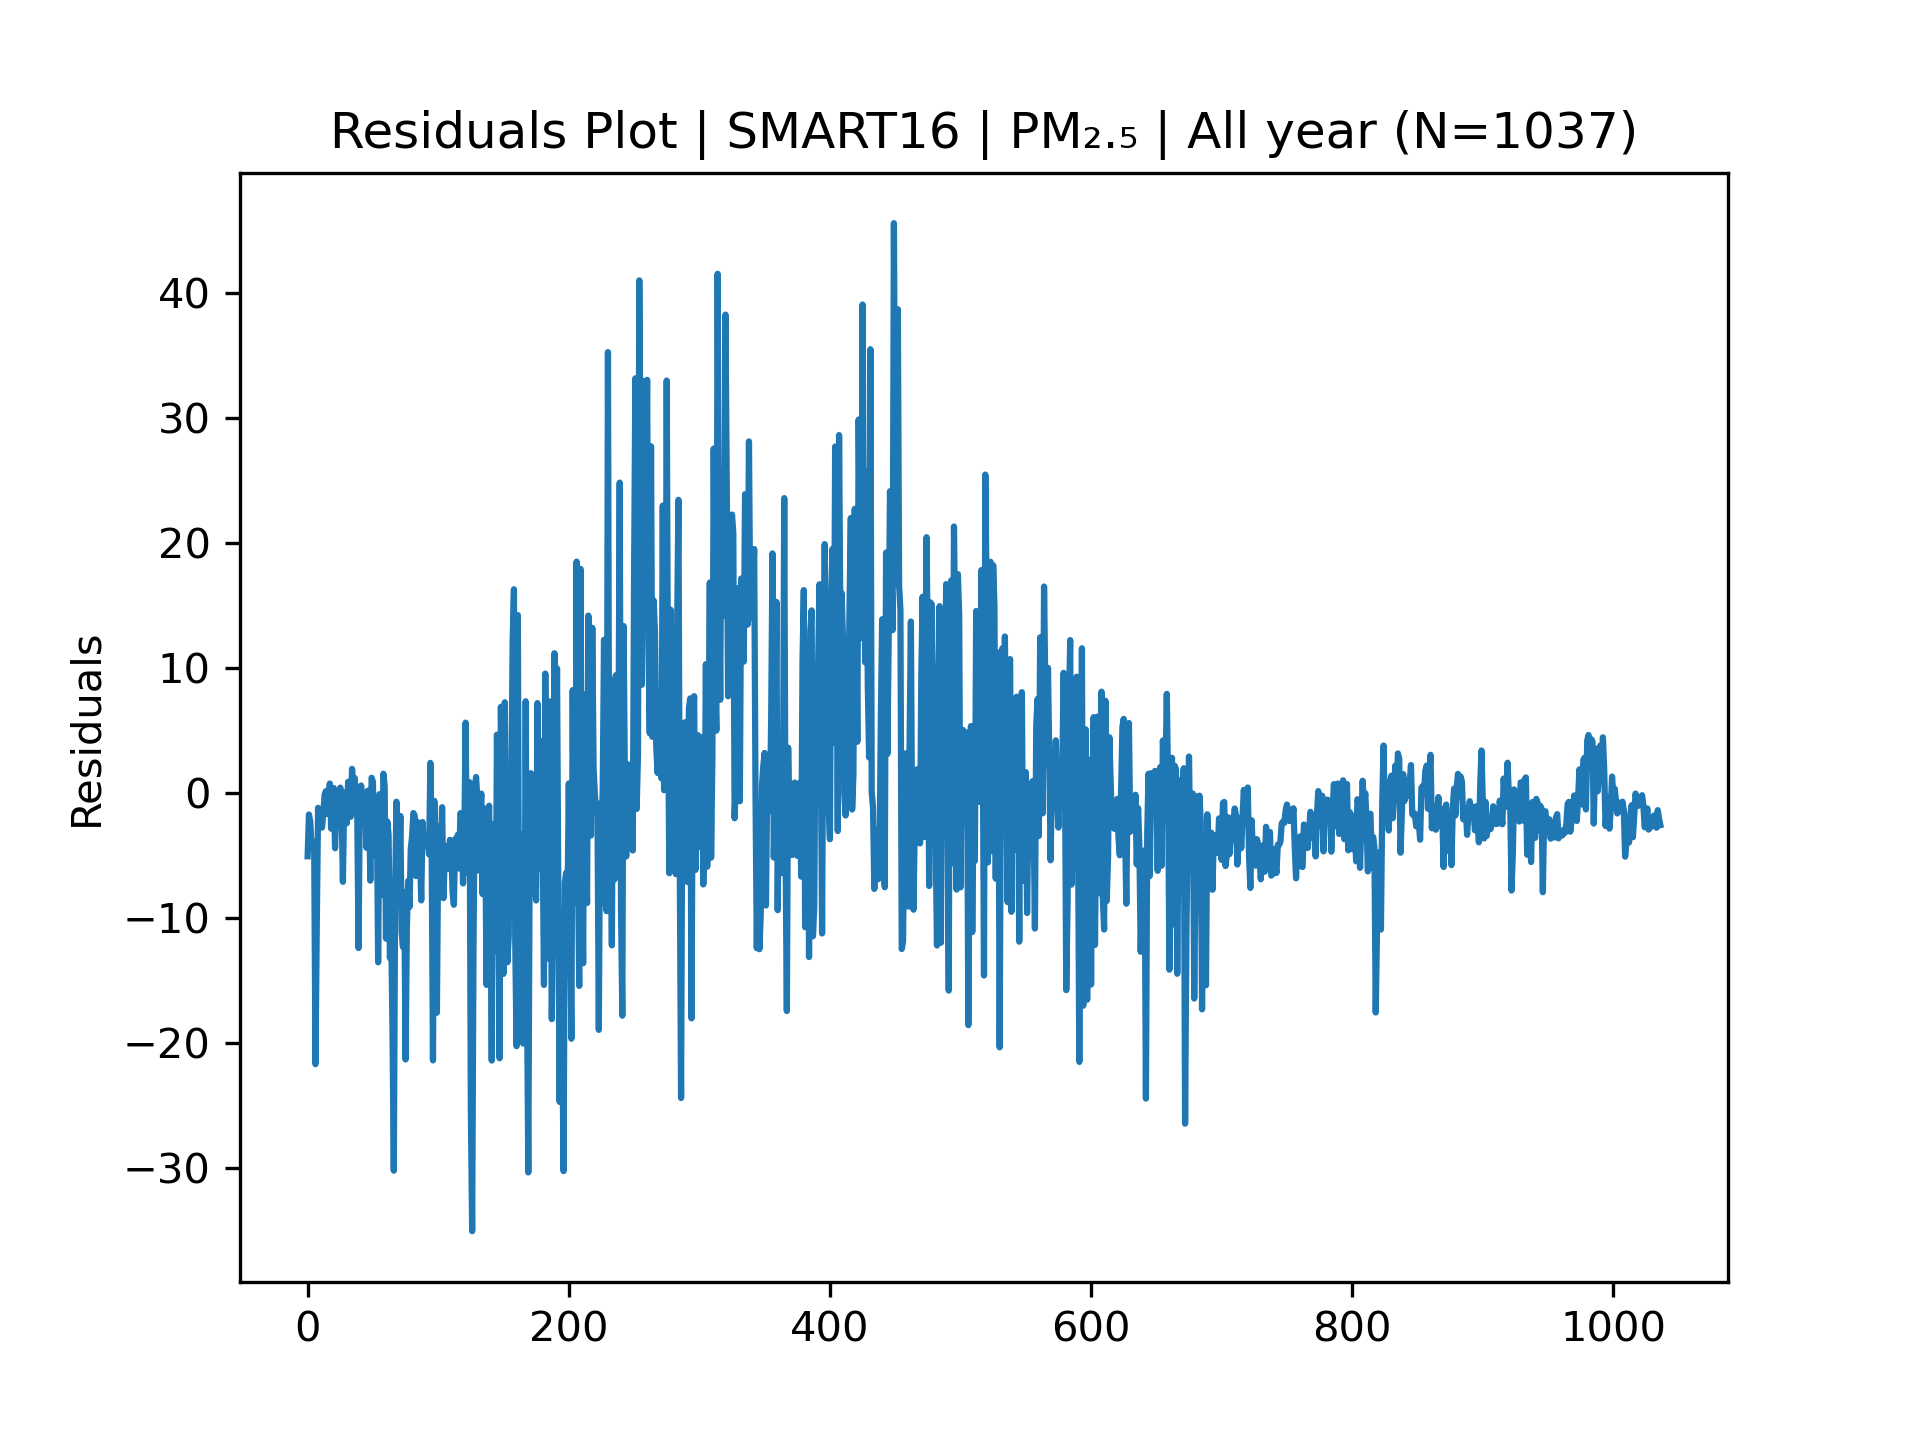
\includegraphics[width=0.42\textwidth]{img/res_pm2.5_plot}%
}

\subfloat[Distribuzione]{%
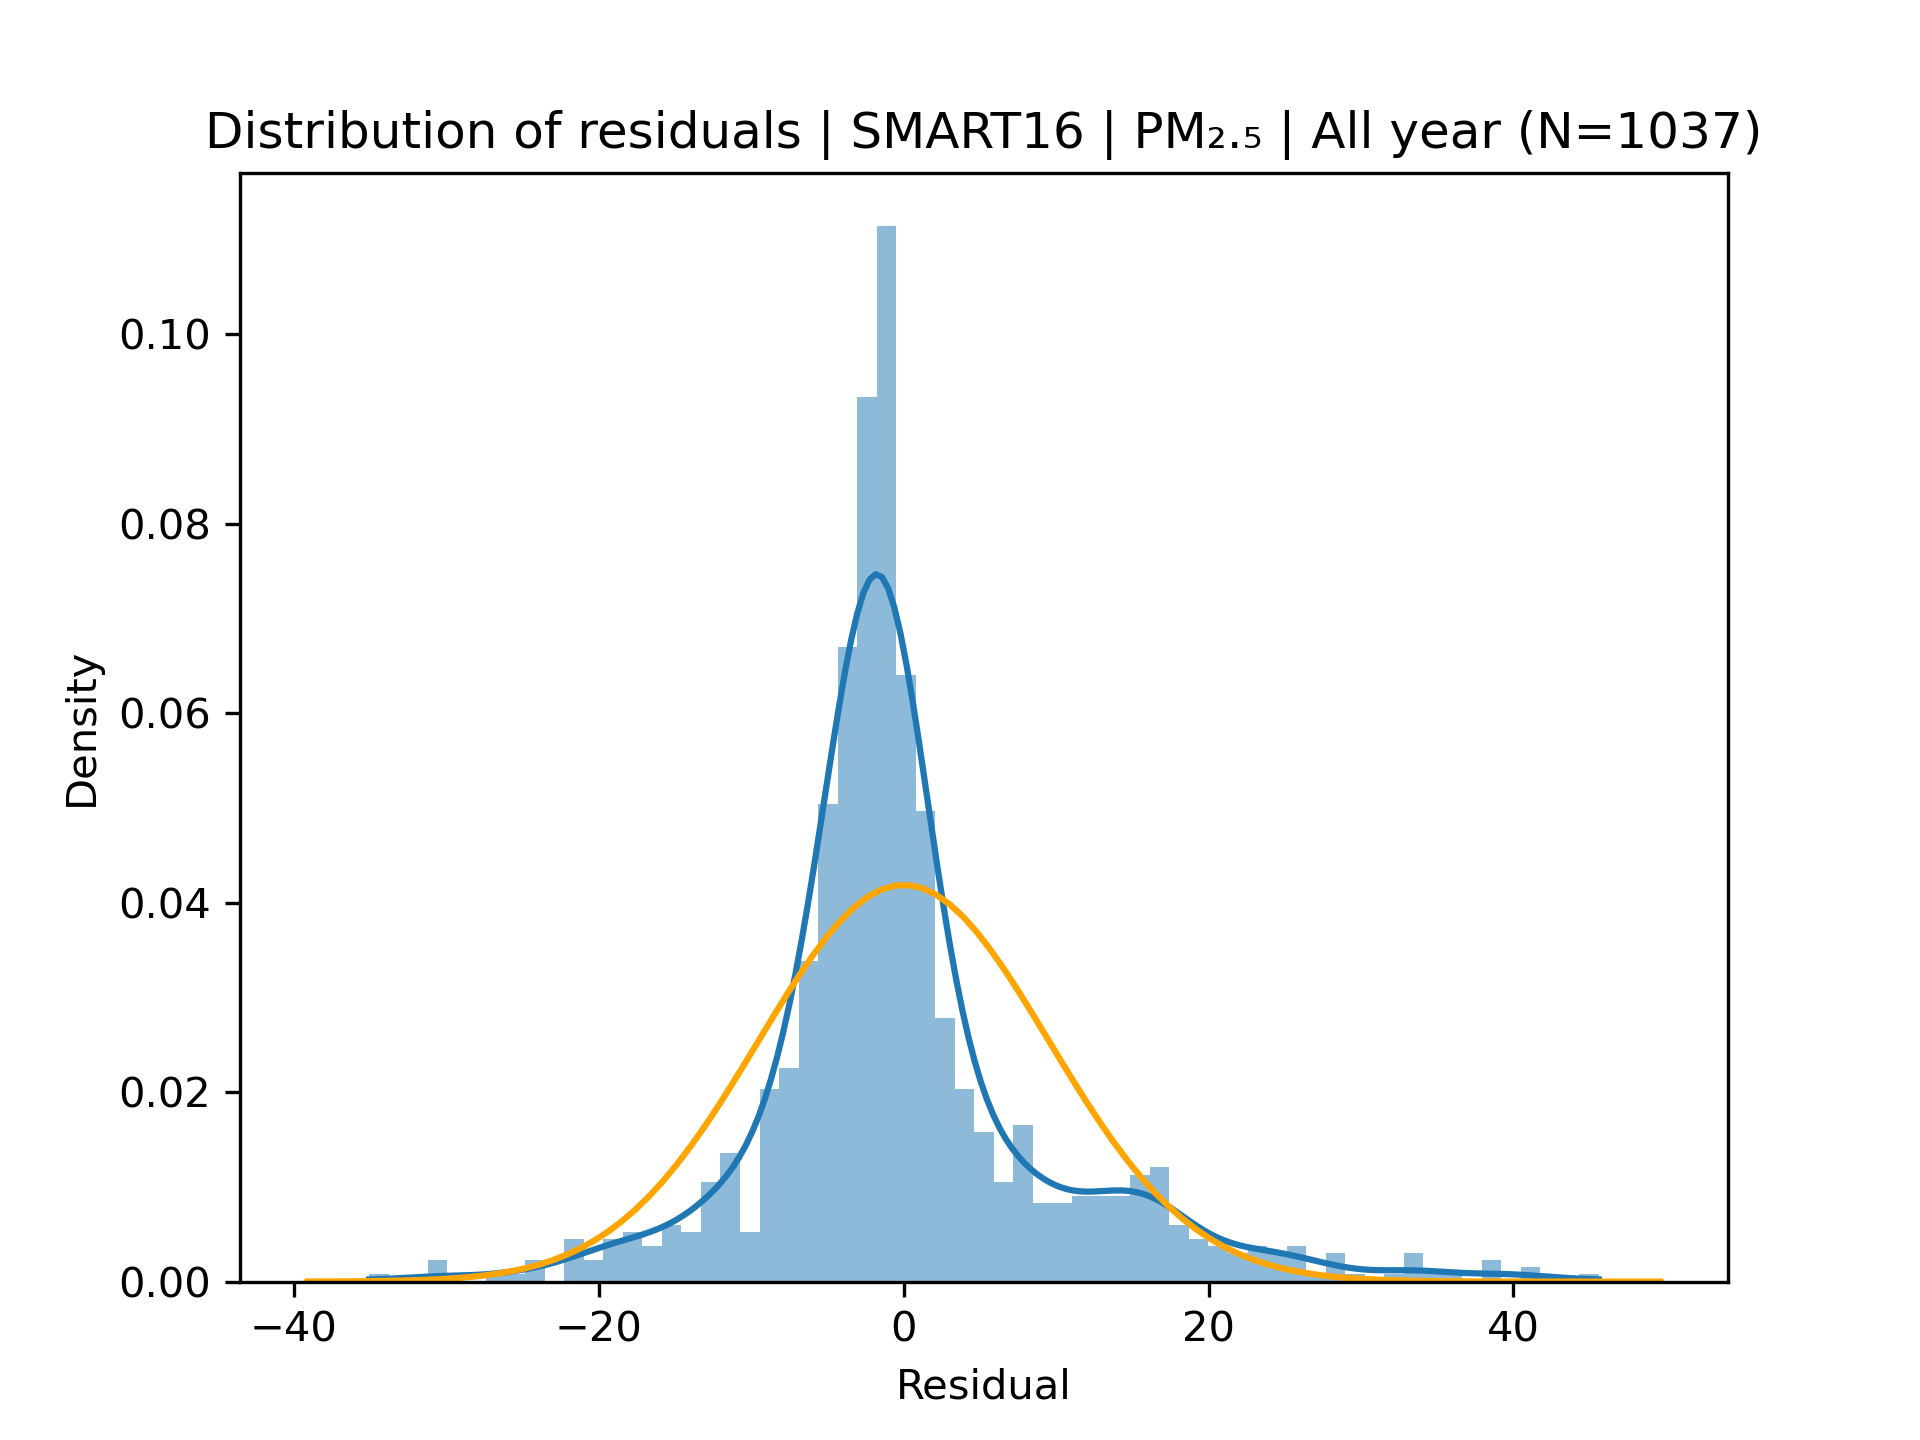
\includegraphics[width=0.42\textwidth]{img/res_pm2.5_distr}%
}\hfil
\subfloat[Q-Q plot]{%
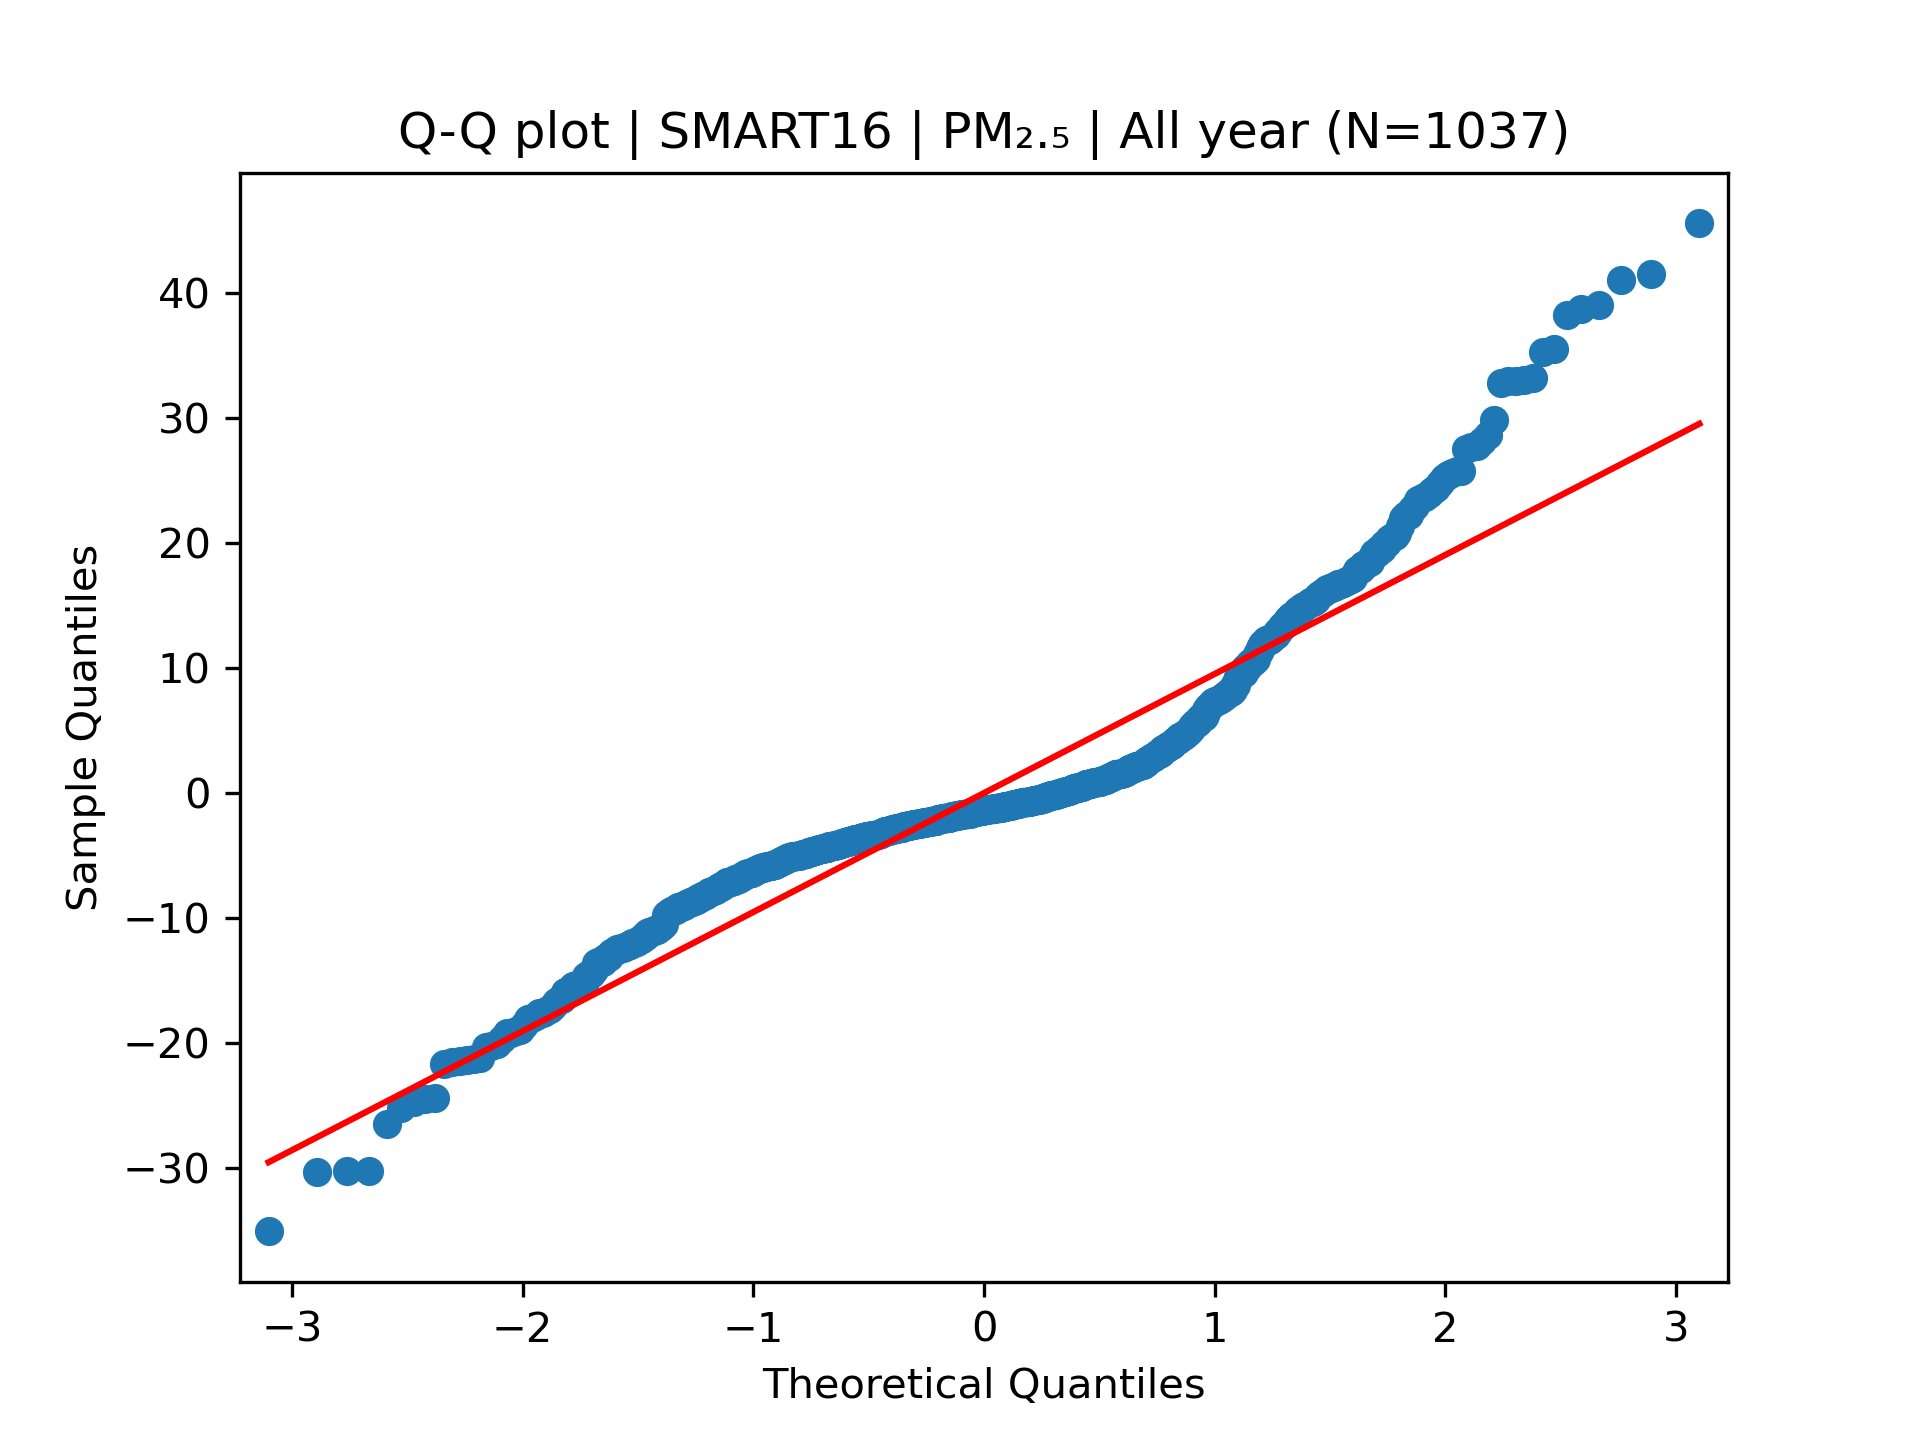
\includegraphics[width=0.42\textwidth]{img/res_pm2.5_qq}%
}
\caption{Analisi dei residui dataset \ce{PM_{2.5}}}
\label{fig:residui_pm2.5}
\end{figure}

La tabella \ref{fig:risultati-pm2.5} mostra i risultati della procedura di calibrazione applicata al sensore di \ce{PM_{2.5}} per ciascun modello di regressione, su tutto il dataset.

\begin{table}[H]
    \footnotesize
    \centering
    \begin{tabular}{|l|c|c|}
    \hline
        \textbf{Modello di regressione} & $\bm{\mathrm{R^2}}$ & \textbf{RMSE (}$\mathrm{\si{\micro}g/m^3}$) \\ \hline
        Lineare & 0.729 & 8.737 \\ \hline
        Lineare robusto (Huber) & 0.730 & 8.706 \\ \hline
        \textbf{Lineare avanzato (Cook)} & \textbf{0.801} & \textbf{5.894} \\ \hline
        Ridge & 0.730 & 8.696 \\ \hline
        Lasso & 0.728 & 8.735 \\ \hline
        Polinomiale (grado 2) & 0.758 & 8.254 \\ \hline
        Polinomiale (grado 3) & 0.756 & 8.227 \\ \hline
        Random Forest & 0.613 & 10.411 \\ \hline
        Gradient Boosting & 0.246 & 14.602 \\ \hline
        SVR (Kernel lineare) & 0.719 & 8.877 \\ \hline
        SVR (Kernel polinomiale) & 0.430 & 12.588 \\ \hline
        SVR (Kernel RBF) & 0.739 & 8.581 \\ \hline
        KernelRidge & 0.757 & 8.208 \\ \hline
    \end{tabular}
    \caption{Risultati della calibrazione \ce{PM_{2.5}}}
    \label{fig:risultati-pm2.5}
\end{table}

E in figura \ref{fig:risultati-pm2.5-hist} gli stessi risultati in forma di istogramma:

\begin{figure}[H]%
    \centering
    \captionsetup{justification=centering}
    \subfloat[\centering $\mathrm{R^2}$]{{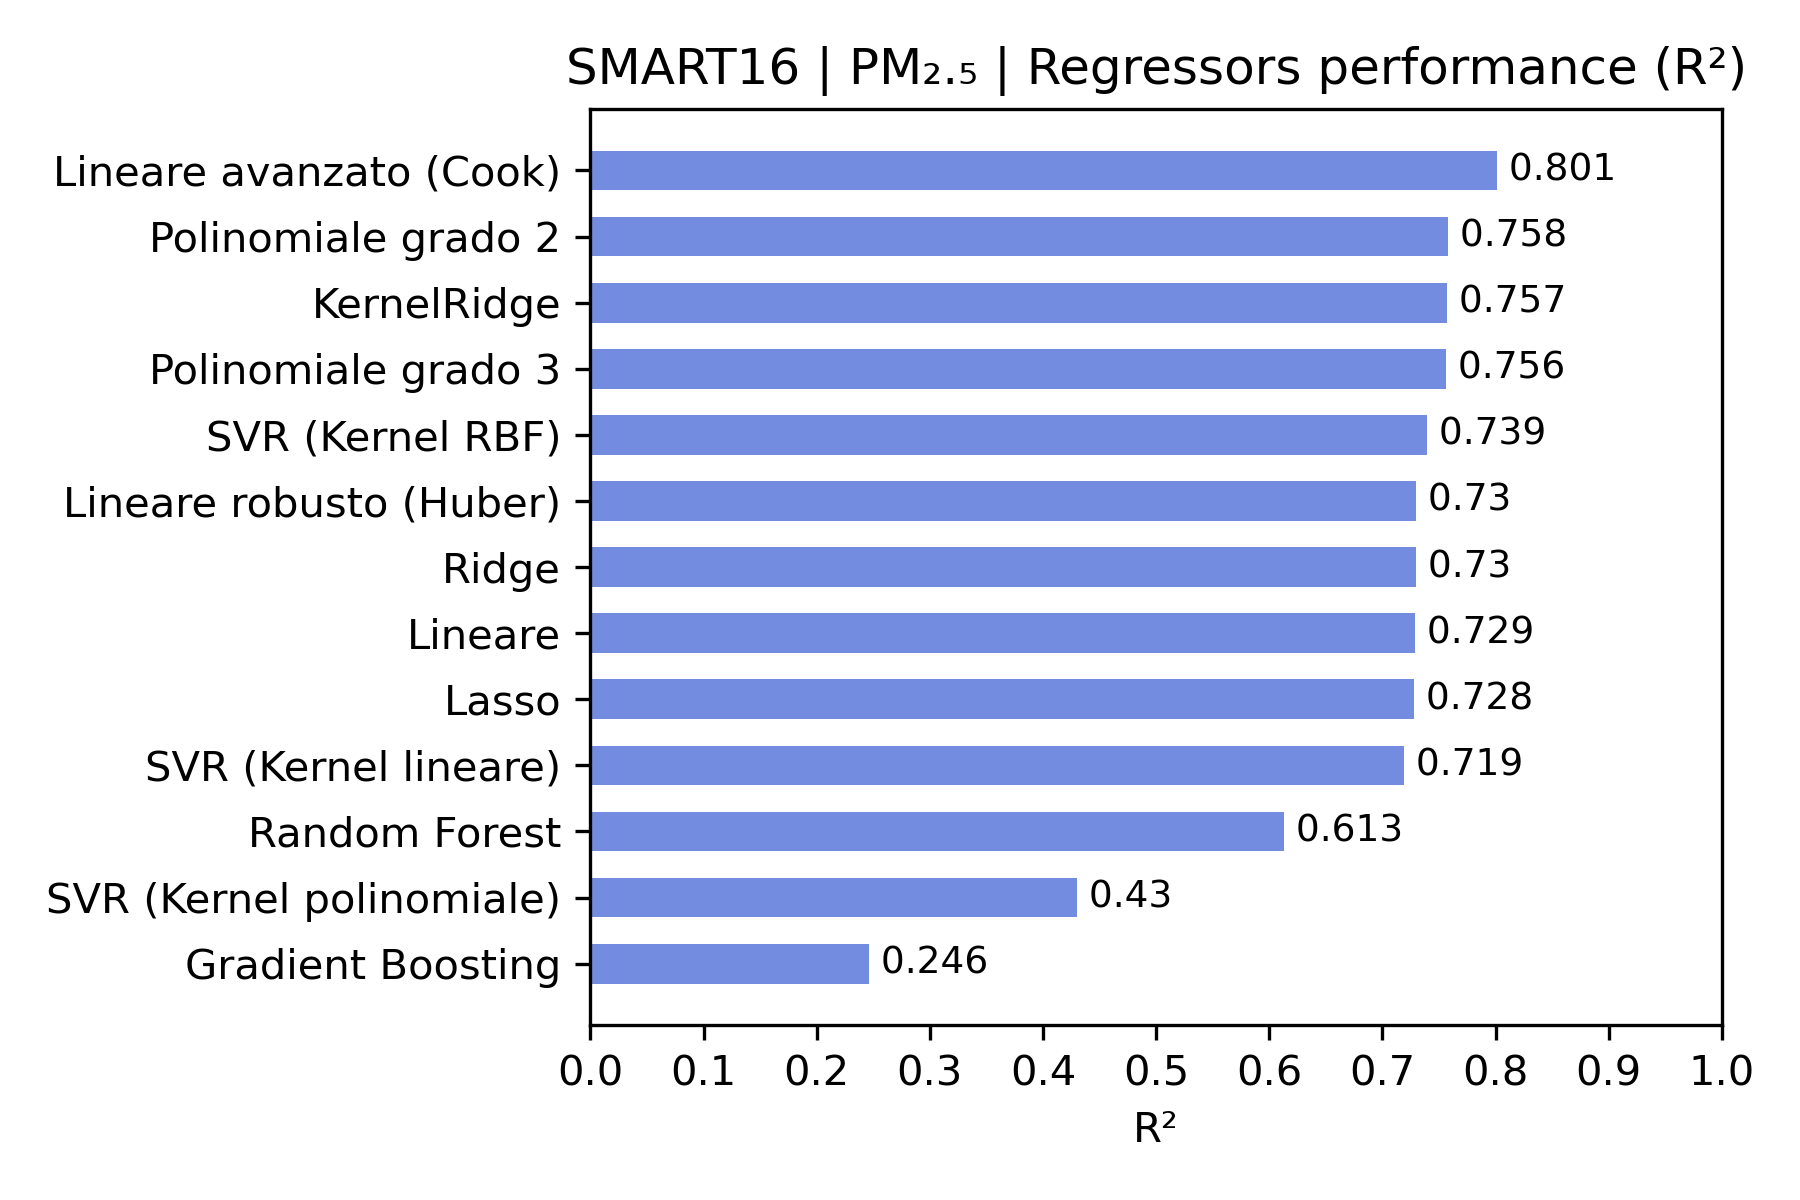
\includegraphics[width=6.9cm]{img/hist_pm2.5_1} }}%
    \subfloat[\centering RMSE]{{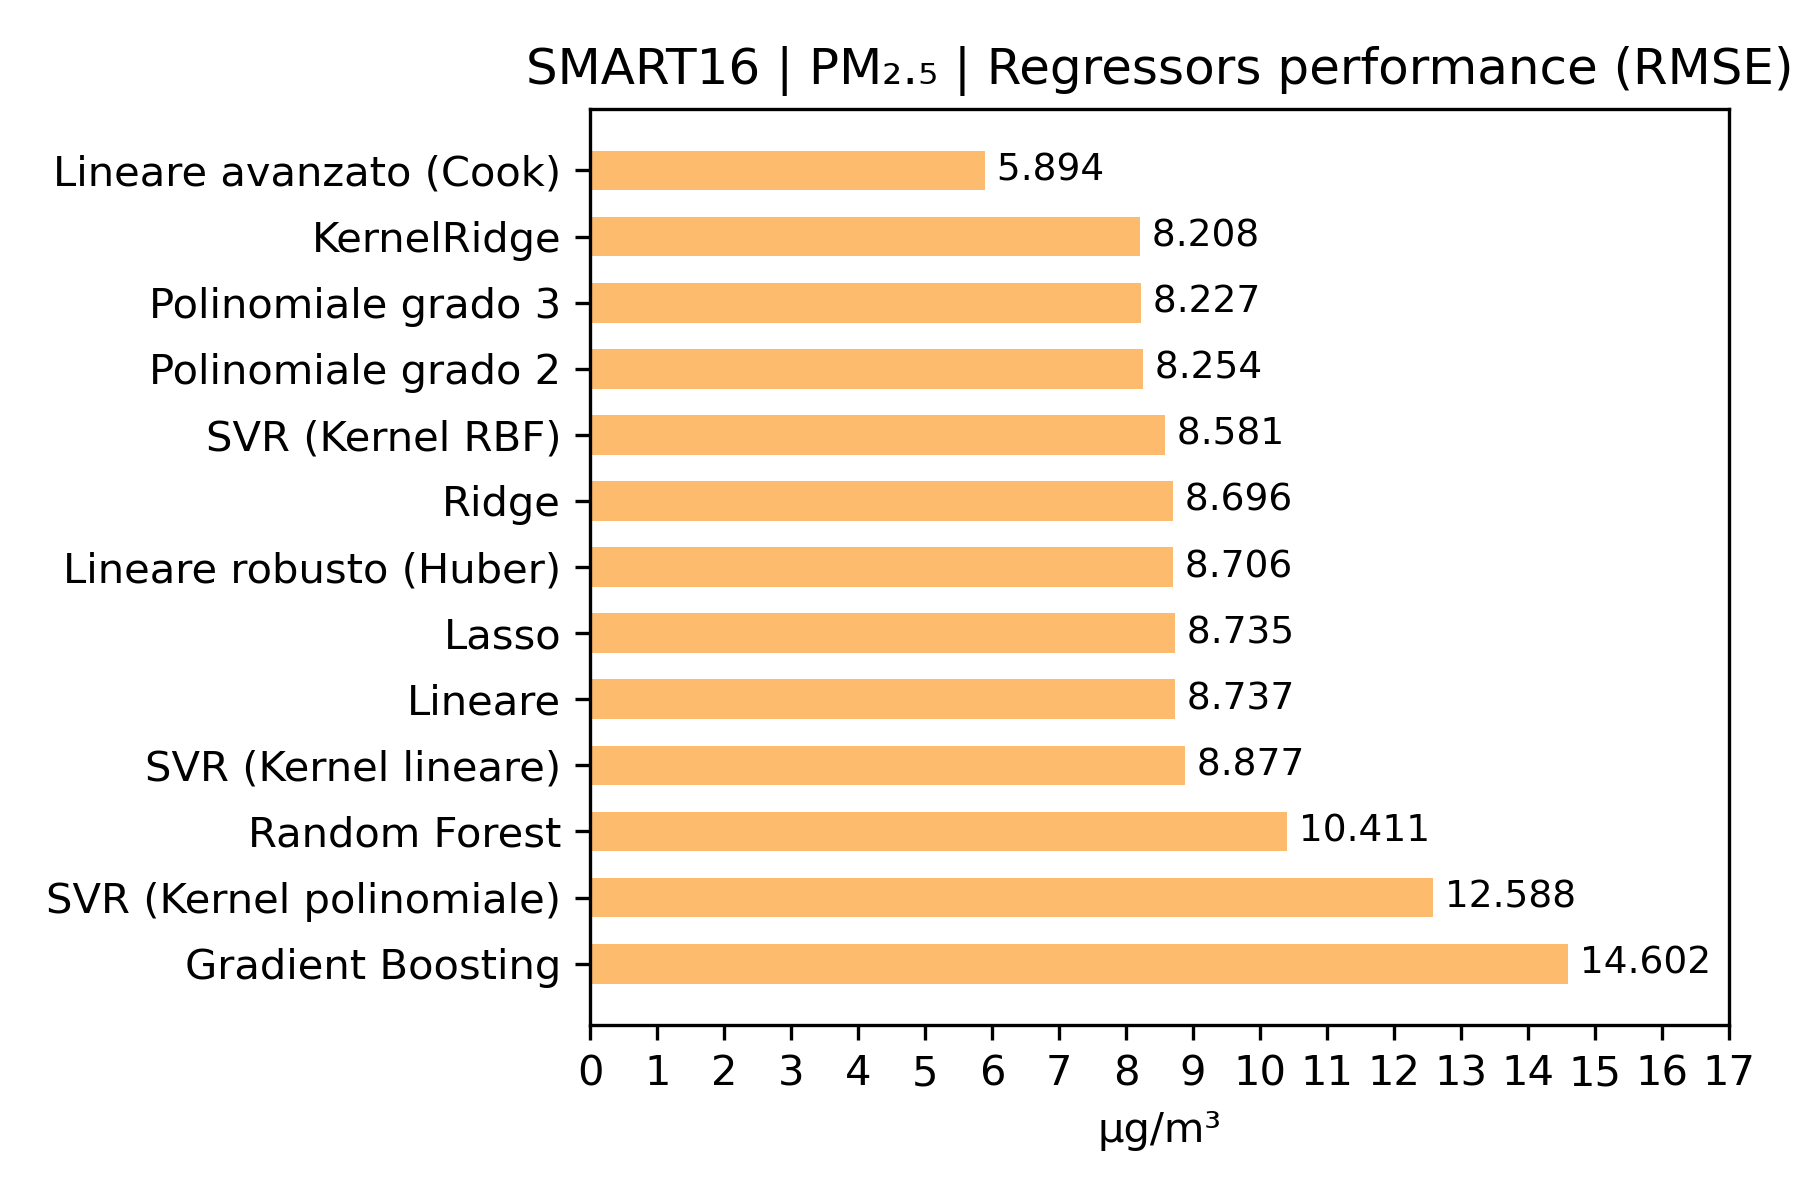
\includegraphics[width=6.9cm]{img/hist_pm2.5_2} }}%
    \caption{Istogramma dei risultati della calibrazione \ce{PM_{2.5}}}%
    \label{fig:risultati-pm2.5-hist}%
\end{figure}

Anche in questo caso nel modello lineare \textit{avanzato}, è stata riapplicata la regressione dopo aver tolto tutti i punti con distanza di Cook (\ref{sssec:regressione-cook}) sopra la soglia pari a $\frac{4}{numero\ di\ osservazioni} = \frac{4}{1037} \approx 0,0038$. In particolare sono stati individuati e rimossi 80 outlier su 1037 osservazioni totali, circa il 7.71\% (figura \ref{fig:cook-pm2.5}).

\begin{figure}[H]
\centering
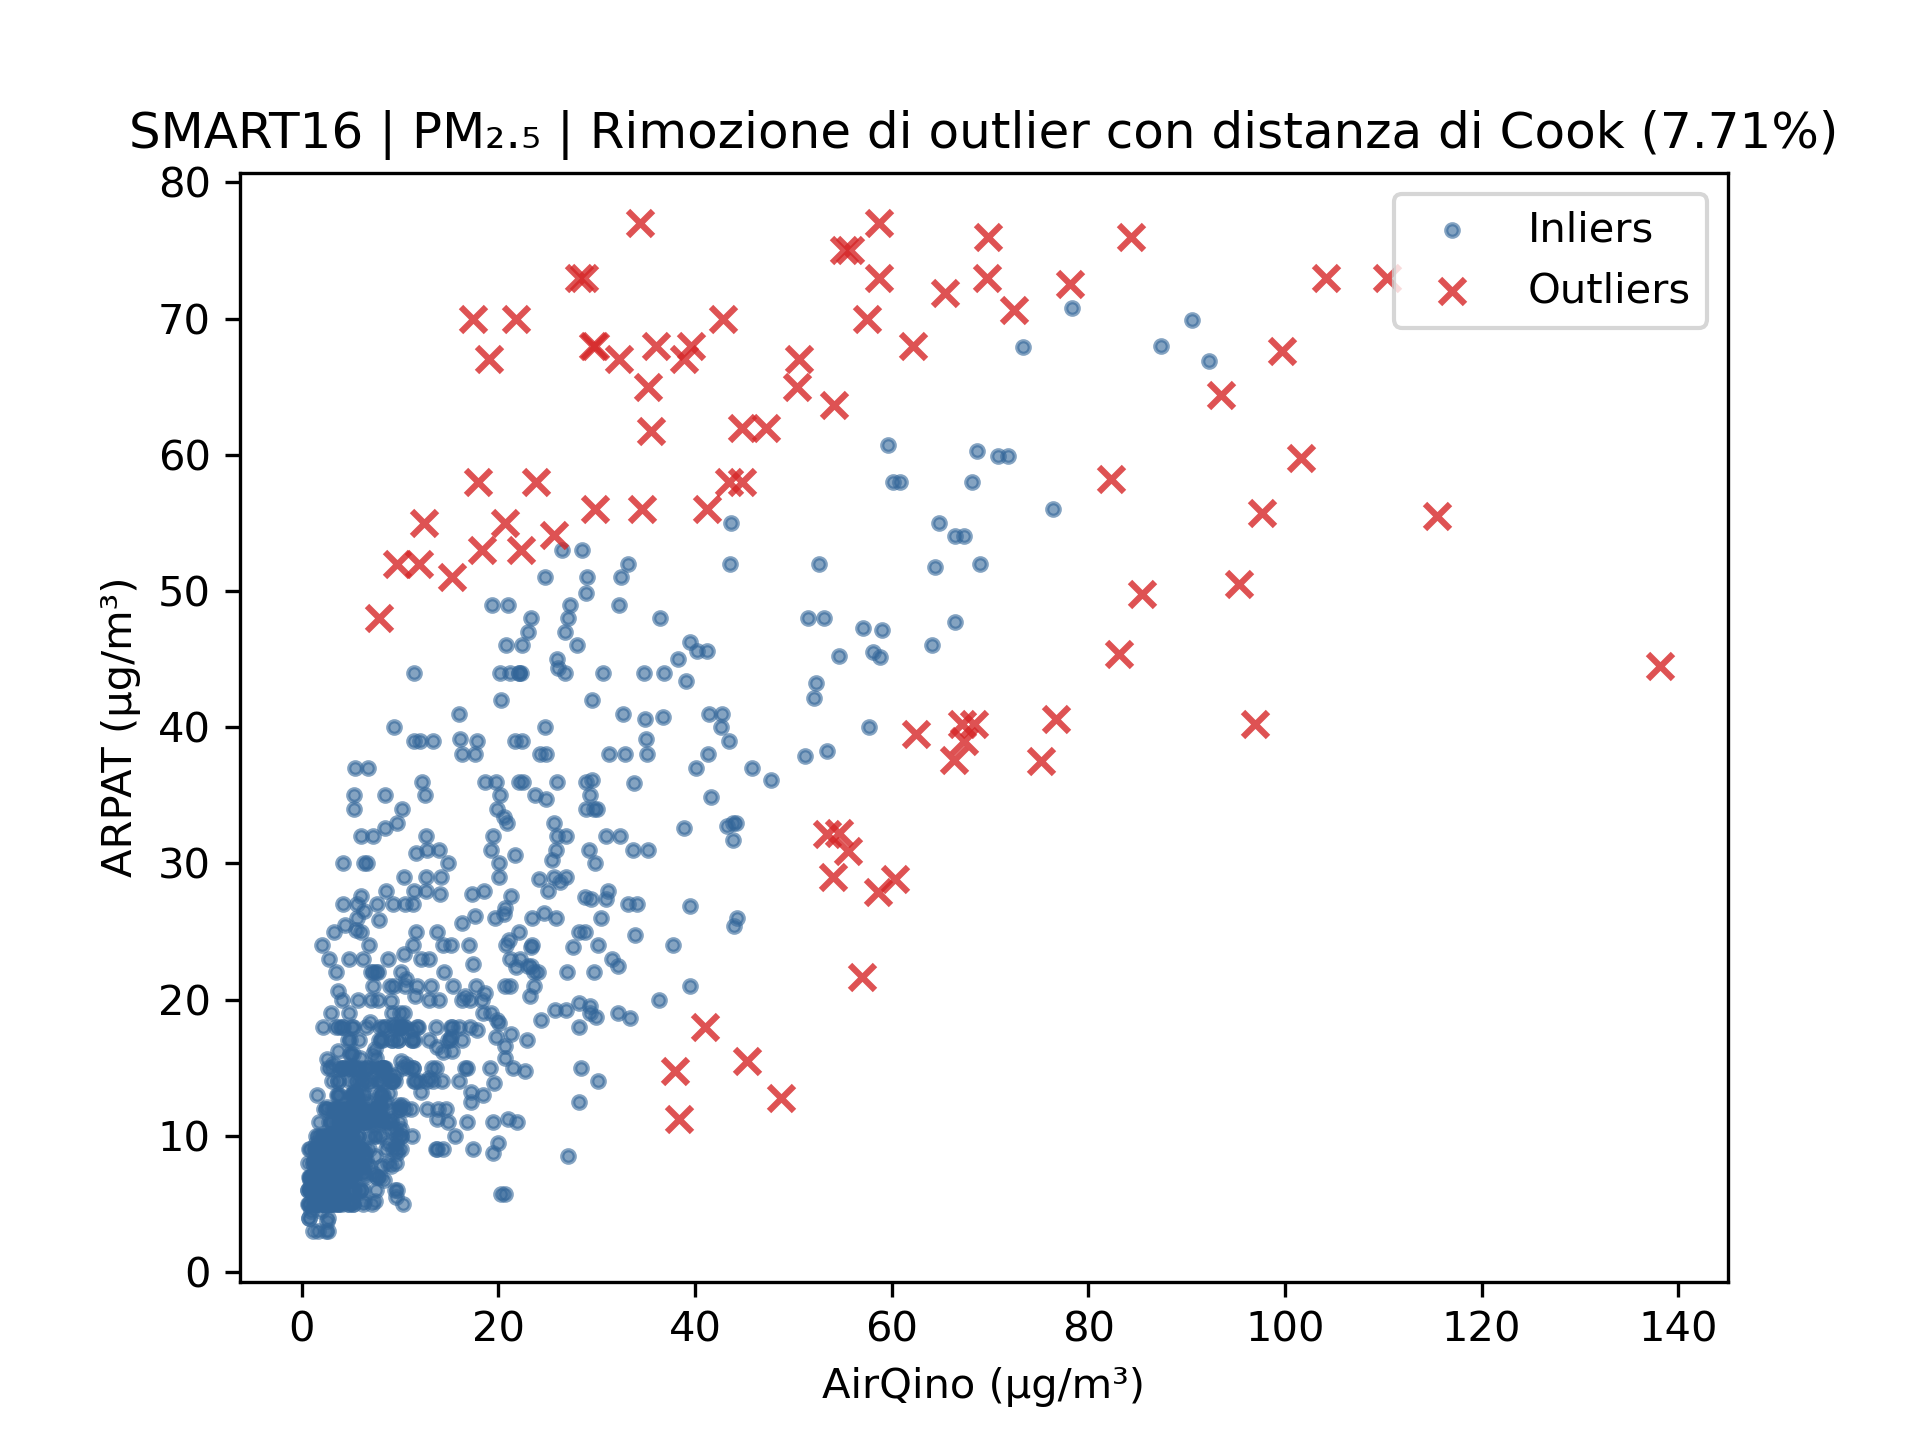
\includegraphics[width=0.75\textwidth,height=\textheight,keepaspectratio]{img/cook_pm2.5.png}
\caption{Rimozione di outlier con distanza di Cook su dataset \ce{PM_{2.5}}}%
\label{fig:cook-pm2.5}%
\end{figure}

Nelle tabelle \ref{fig:risultati-pm2.5-mese} e \ref{fig:risultati-pm2.5-rmse-mese} sono invece riportati rispettivamente $R^2$ e RMSE della calibrazione su dataset \ce{PM_{2.5}} fatta mese per mese.

\begin{table}[H]
    \tiny
    \centering
    \setlength{\tabcolsep}{4pt}
    \def\arraystretch{1.5}
    \begin{tabular}{|l|c|c|c|c|c|c|c|c|c|c|c|c|}
    \hline
        \textbf{Modello} & \textbf{Set} & \textbf{Ott} & \textbf{Nov} & \textbf{Dic} & \textbf{Gen} & \textbf{Feb} & \textbf{Mar} & \textbf{Apr} & \textbf{Mag} & \textbf{Giu} & \textbf{Lug} & \textbf{Ago} \\ \hline
        Lineare & 0.29 & 0.49 & 0.18 & 0.72 & 0.61 & 0.60 & 0.56 & 0.19 & 0.02 & 0.26 & 0.55 & 0.61 \\ \hline
        Lineare robusto (Huber) & 0.28 & 0.48 & 0.19 & 0.72 & 0.62 & 0.58 & 0.58 & 0.18 & -0.00 & 0.27 & 0.55 & 0.61 \\ \hline
        \textbf{Lineare avanzato (Cook)} & \textbf{0.58} & \textbf{0.62} & 0.15 & \textbf{0.73} & 0.66 & \textbf{0.68} & \textbf{0.62} & \textbf{0.29} & \textbf{0.02} & 0.28 & \textbf{0.69} & \textbf{0.70} \\ \hline
        Ridge & 0.26 & 0.48 & 0.18 & 0.71 & 0.61 & 0.59 & 0.57 & 0.18 & 0.01 & 0.26 & 0.52 & 0.60 \\ \hline
        Lasso & 0.28 & 0.47 & 0.18 & 0.72 & 0.60 & 0.59 & 0.56 & 0.18 & 0.01 & 0.26 & 0.54 & 0.62 \\ \hline
        Polinomiale (grado 2) & 0.32 & 0.46 & 0.22 & \textbf{0.73} & \textbf{0.68} & 0.55 & 0.54 & 0.09 & -0.03 & 0.28 & 0.59 & 0.59 \\ \hline
        Polinomiale (grado 3) & -0.70 & 0.31 & 0.19 & 0.66 & 0.65 & 0.54 & 0.53 & -0.24 & -0.10 & 0.26 & 0.33 & 0.60 \\ \hline
        Random Forest & 0.23 & 0.37 & -0.03 & 0.65 & 0.50 & 0.29 & 0.28 & -0.17 & -0.68 & -0.24 & 0.46 & 0.49 \\ \hline
        Gradient Boosting & 0.09 & 0.10 & 0.03 & 0.20 & 0.17 & 0.08 & 0.12 & -0.02 & -0.08 & 0.02 & 0.14 & 0.15 \\ \hline
        SVR (lineare) & 0.14 & 0.45 & 0.14 & 0.69 & 0.60 & 0.53 & 0.53 & 0.15 & 0.01 & 0.24 & 0.52 & 0.61 \\ \hline
        SVR (polinomiale) & -0.55 & -0.15 & 0.08 & 0.50 & 0.26 & 0.40 & 0.51 & 0.12 & -0.02 & 0.17 & -0.09 & 0.57 \\ \hline
        SVR (RBF) & 0.16 & 0.44 & 0.22 & 0.65 & 0.58 & 0.39 & 0.37 & -0.06 & -0.36 & -0.07 & 0.62 & 0.50 \\ \hline
        KernelRidge & 0.36 & 0.45 & \textbf{0.25} & \textbf{0.73} & 0.67 & 0.57 & 0.54 & 0.06 & -0.06 & \textbf{0.29} & 0.62 & 0.60 \\ \hline
    \end{tabular}
    \caption{Risultati della calibrazione \ce{PM_{2.5}} mese per mese ($R^2$)}
    \label{fig:risultati-pm2.5-mese}
\end{table}

\begin{table}[H]
    \tiny
    \centering
    \setlength{\tabcolsep}{4pt}
    \def\arraystretch{1.5}
    \begin{tabular}{|l|c|c|c|c|c|c|c|c|c|c|c|c|}
    \hline
        \textbf{Modello} & \textbf{Set} & \textbf{Ott} & \textbf{Nov} & \textbf{Dic} & \textbf{Gen} & \textbf{Feb} & \textbf{Mar} & \textbf{Apr} & \textbf{Mag} & \textbf{Giu} & \textbf{Lug} & \textbf{Ago} \\ \hline
        Lineare & 3.78 & 6.27 & 13.35 & 11.55 & 12.39 & 7.70 & 6.27 & 3.74 & 1.38 & 1.92 & 1.54 & 2.05 \\ \hline
        Lineare robusto (Huber) & 3.77 & 6.25 & 13.19 & 11.58 & 12.17 & 7.87 & 6.27 & 3.77 & 1.38 & 1.93 & 1.53 & 2.04 \\ \hline
        \textbf{Lineare avanzato (Cook)} & \textbf{2.92} & \textbf{4.99} & 12.78 & \textbf{10.62} & 11.55 & \textbf{7.08} & \textbf{5.53} & \textbf{3.38} & \textbf{1.25} & \textbf{1.80} & \textbf{1.26} & \textbf{1.72} \\ \hline
        Ridge & 3.86 & 6.31 & 13.36 & 11.69 & 12.33 & 7.82 & 6.29 & 3.80 & 1.38 & 1.96 & 1.60 & 2.06 \\ \hline
        Lasso & 3.82 & 6.32 & 13.32 & 11.56 & 12.48 & 7.85 & 6.29 & 3.77 & 1.36 & 1.95 & 1.57 & 2.04 \\ \hline
        Polinomiale (grado 2) & 3.63 & 6.42 & 12.94 & 11.38 & \textbf{11.29} & 8.03 & 6.43 & 3.95 & 1.38 & 1.88 & 1.45 & 2.11 \\ \hline
        Polinomiale (grado 3) & 5.10 & 6.89 & 13.13 & 12.57 & 11.46 & 8.13 & 6.56 & 4.43 & 1.42 & 1.94 & 1.73 & 2.03 \\ \hline
        Random Forest & 3.85 & 6.86 & 14.86 & 12.62 & 13.54 & 10.14 & 7.93 & 4.44 & 1.76 & 2.48 & 1.68 & 2.27 \\ \hline
        Gradient Boosting & 4.33 & 8.32 & 14.71 & 19.83 & 18.33 & 11.96 & 9.30 & 4.24 & 1.44 & 2.29 & 2.14 & 3.09 \\ \hline
        SVR (lineare) & 3.98 & 6.46 & 13.55 & 12.10 & 12.46 & 8.30 & 6.50 & 3.79 & 1.39 & 1.98 & 1.57 & 2.05 \\ \hline
        SVR (polinomiale) & 5.27 & 9.25 & 14.23 & 15.22 & 16.60 & 9.09 & 6.74 & 3.94 & 1.39 & 2.08 & 2.20 & 2.13 \\ \hline
        SVR (RBF) & 3.99 & 6.51 & 12.98 & 12.88 & 12.60 & 9.41 & 7.54 & 4.25 & 1.57 & 2.33 & 1.41 & 2.23 \\ \hline
        KernelRidge & 3.56 & 6.45 & \textbf{12.65} & 11.31 & 11.31 & 7.92 & 6.36 & 4.01 & 1.42 & 1.88 & 1.39 & 2.06 \\ \hline
    \end{tabular}
    \caption{Risultati della calibrazione \ce{PM_{2.5}} mese per mese (RMSE)}
    \label{fig:risultati-pm2.5-rmse-mese}
\end{table}

\clearpage
Infine, la tabella \ref{fig:risultati-pm2.5-coefficienti} riporta i coefficienti delle curve di regressione ottenuti applicando i modelli al dataset \ce{PM_{2.5}}. Anche in questo caso i coefficienti \textit{a}, \textit{b}, \textit{c}, \textit{d}, \textit{e} si riferiscono ad una equazione polinomiale generica del tipo $y=a+bx+cx^2+dx^3+ex^4$.

\begin{table}[H]
    \footnotesize
    \centering
    \begin{tabular}{|l|c|c|c|c|c|c|c|}
    \hline
        \textbf{Modello di regressione} & \textbf{a} & \textbf{b} & \textbf{c} & \textbf{d} & \textbf{e} \\ \hline
        Lineare & 13.15 & 9.50 & / & / & / \\ \hline
        Lineare robusto (Huber) & 13.33 & 9.23 & / & / & / \\ \hline
        Lineare avanzato (Cook) & 10.31 & 7.67 & / & / & / \\ \hline
        Lasso & 13.02 & 9.60 & / & / & / \\ \hline
        Ridge & 13.01 & 9.61 & / & / & / \\ \hline
        Polinomiale (grado 2) & 5.93 & 22.37 & -2.34 & / & / \\ \hline
        Polinomiale (grado 3) & 5.19 & 25.32 & -4.07 & 0.23 & / \\ \hline
        Polinomiale (grado 4) & 4.17 & 30.76 & -9.29 & 1.75 & -0.13 \\ \hline
    \end{tabular}
    \caption{Coefficienti della calibrazione \ce{PM_{2.5}}}
    \label{fig:risultati-pm2.5-coefficienti}
\end{table}


\subsection{Risultati \ce{PM10}}\label{ssec:risultati-pm10}

Il confronto tra le misurazioni AirQino e le misurazioni di riferimento ARPAT per \ce{PM_{10}} sono riportate nello \textit{scatterplot} di figura \ref{fig:scatterplot_pm10}.

\clearpage

\begin{figure}[H]
\centering
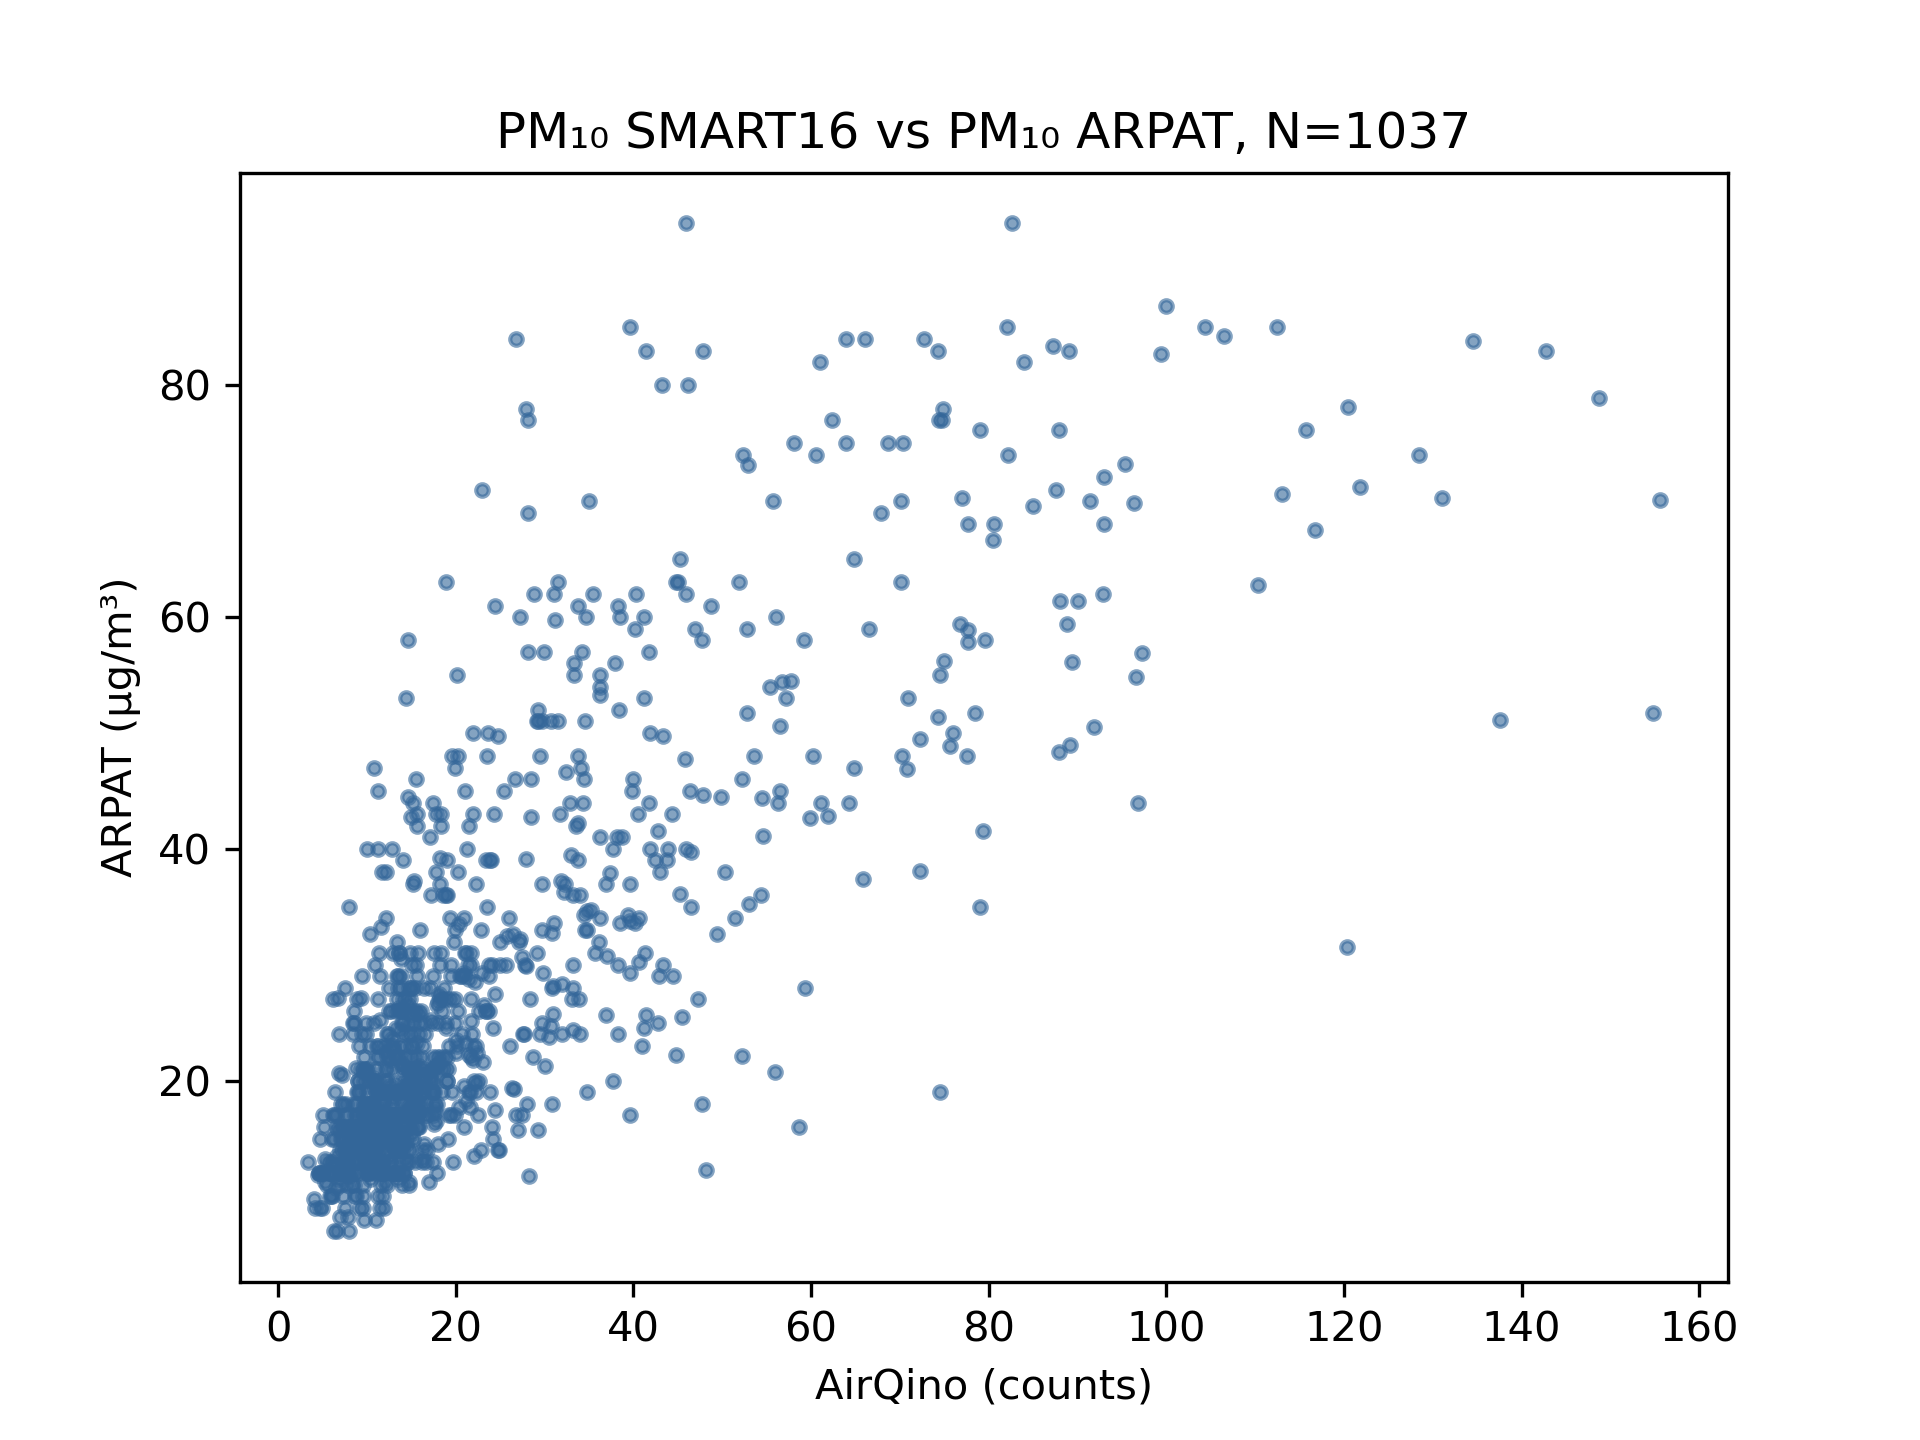
\includegraphics[width=0.55\textwidth,height=\textheight,keepaspectratio]{img/sc_pm10.png}
\caption{Scatterplot dataset \ce{PM_{10}}}
\label{fig:scatterplot_pm10}
\end{figure}

I risultati dell'analisi grafica dei residui sono riportati in figura \ref{fig:residui_pm10}.

\begin{figure}[H]
\centering
\subfloat[Scatterplot]{%
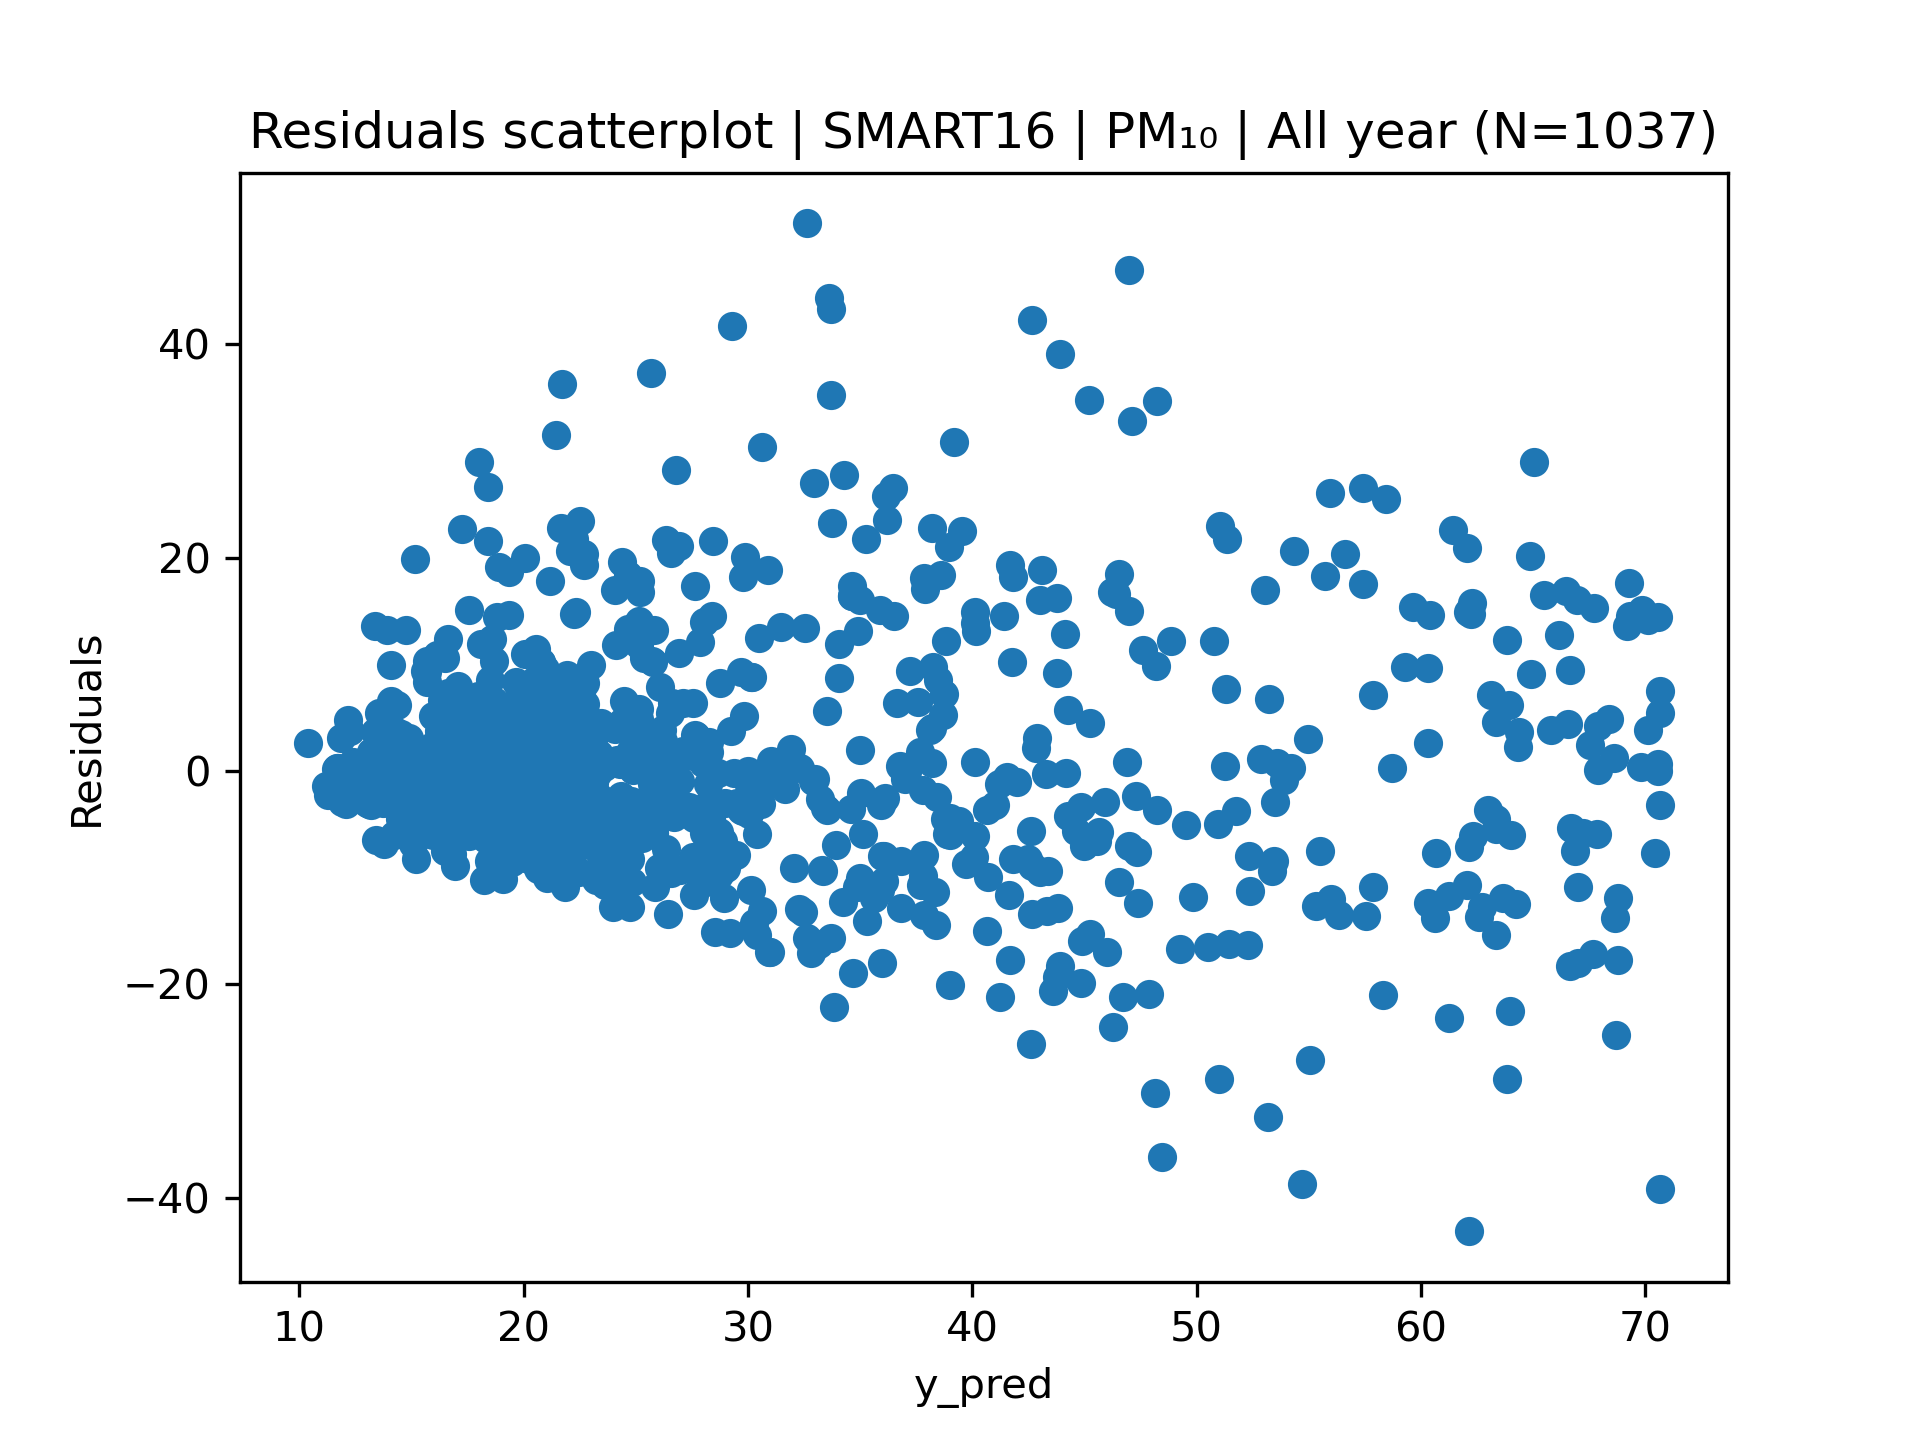
\includegraphics[width=0.42\textwidth]{img/res_pm10_scatter}%
}\hfil
\subfloat[Plot]{%
\includegraphics[width=0.42\textwidth]{img/res_pm10_plot}%
}

\subfloat[Distribuzione]{%
\includegraphics[width=0.42\textwidth]{img/res_pm10_distr}%
}\hfil
\subfloat[Q-Q plot]{%
\includegraphics[width=0.42\textwidth]{img/res_pm10_qq}%
}
\caption{Analisi dei residui dataset \ce{PM_{10}}}
\label{fig:residui_pm10}
\end{figure}

La tabella \ref{fig:risultati-pm10} mostra i risultati della procedura di calibrazione applicata al sensore di \ce{PM_{10}} per ciascun modello di regressione, su tutto il dataset.

\begin{table}[H]
    \footnotesize
    \centering
    \begin{tabular}{|l|c|c|}
    \hline
        \textbf{Modello di regressione} & $\bm{\mathrm{R^2}}$ & \textbf{RMSE (}$\mathrm{\si{\micro}g/m^3}$) \\ \hline
        Lineare & 0.715 & 9.706 \\ \hline
        Lineare robusto (Huber) & 0.716 & 9.760 \\ \hline
        \textbf{Lineare avanzato (Cook)} & \textbf{0.785} & \textbf{7.103} \\ \hline
        Ridge & 0.715 & 9.707 \\ \hline
        Lasso & 0.716 & 9.754 \\ \hline
        Polinomiale (grado 2) & 0.739 & 9.343 \\ \hline
        Polinomiale (grado 3) & 0.738 & 9.339 \\ \hline
        Random Forest & 0.590 & 11.686 \\ \hline
        Gradient Boosting & 0.238 & 16.004 \\ \hline
        SVR (Kernel lineare) & 0.707 & 9.860 \\ \hline
        SVR (Kernel polinomiale) & 0.513 & 12.724 \\ \hline
        SVR (Kernel RBF) & 0.719 & 9.672 \\ \hline
        KernelRidge & 0.738 & 9.321 \\ \hline
    \end{tabular}
    \caption{Risultati della calibrazione \ce{PM_{10}}}
    \label{fig:risultati-pm10}
\end{table}

E in figura \ref{fig:risultati-pm10-hist} gli stessi risultati in forma di istogramma:

\begin{figure}[H]%
    \centering
    \captionsetup{justification=centering}
    \subfloat[\centering $\mathrm{R^2}$]{{\includegraphics[width=6.9cm]{img/hist_pm10_1} }}%
    \subfloat[\centering RMSE]{{\includegraphics[width=6.9cm]{img/hist_pm10_2} }}%
    \caption{Istogramma dei risultati della calibrazione \ce{PM_{10}}}%
    \label{fig:risultati-pm10-hist}%
\end{figure}

Anche in questo caso nel modello lineare \textit{avanzato}, è stata riapplicata la regressione dopo aver tolto tutti i punti con distanza di Cook (\ref{sssec:regressione-cook}) sopra la soglia pari a $\frac{4}{numero\ di\ osservazioni} = \frac{4}{1037} \approx 0,0038$. In particolare sono stati individuati e rimossi 70 outlier su 1037 osservazioni totali, circa il 6.71\% (figura \ref{fig:cook-pm10}).

\begin{figure}[H]
\centering
\includegraphics[width=0.75\textwidth,height=\textheight,keepaspectratio]{img/cook_pm10.png}
\caption{Rimozione di outlier con distanza di Cook su dataset \ce{PM_{10}}}%
\label{fig:cook-pm10}%
\end{figure}

Nelle tabelle \ref{fig:risultati-pm10-mese} e \ref{fig:risultati-pm10-rmse-mese} sono invece riportati rispettivamente $R^2$ e RMSE della calibrazione su dataset \ce{PM_{10}} fatta mese per mese.

\begin{table}[H]
    \tiny
    \centering
    \setlength{\tabcolsep}{4pt}
    \def\arraystretch{1.5}
    \begin{tabular}{|l|c|c|c|c|c|c|c|c|c|c|c|c|}
    \hline
        \textbf{Modello} & \textbf{Set} & \textbf{Ott} & \textbf{Nov} & \textbf{Dic} & \textbf{Gen} & \textbf{Feb} & \textbf{Mar} & \textbf{Apr} & \textbf{Mag} & \textbf{Giu} & \textbf{Lug} & \textbf{Ago} \\ \hline
        Lineare & -0.02 & 0.36 & 0.24 & 0.67 & 0.55 & 0.64 & 0.55 & 0.07 & 0.26 & 0.20 & 0.64 & 0.71 \\ \hline
        Lineare robusto (Huber) & -0.02 & 0.34 & 0.24 & 0.68 & 0.55 & 0.64 & 0.56 & \textbf{0.10} & 0.27 & 0.21 & 0.64 & 0.70 \\ \hline
        \textbf{Lineare avanzato (Cook)} & \textbf{0.39} & \textbf{0.54} & 0.22 & \textbf{0.69} & \textbf{0.62} & \textbf{0.66} & \textbf{0.67} & \textbf{0.10} & \textbf{0.30} & 0.03 & 0.62 & 0.71 \\ \hline
        Ridge & -0.00 & 0.34 & 0.25 & 0.68 & 0.53 & 0.63 & 0.54 & 0.03 & 0.26 & 0.18 & 0.64 & \textbf{0.72} \\ \hline
        Lasso & 0.01 & 0.35 & 0.23 & 0.69 & 0.53 & 0.64 & 0.53 & 0.05 & 0.26 & 0.20 & 0.62 & 0.71 \\ \hline
        Polinomiale (grado 2) & 0.37 & 0.38 & 0.27 & 0.68 & 0.60 & 0.62 & 0.52 & -0.03 & 0.25 & 0.11 & \textbf{0.65} & 0.67 \\ \hline
        Polinomiale (grado 3) & -1.00 & 0.26 & 0.23 & 0.68 & 0.58 & 0.58 & 0.49 & -0.08 & 0.23 & -1.17 & 0.59 & 0.60 \\ \hline
        Random Forest & 0.16 & 0.03 & 0.11 & 0.55 & 0.41 & 0.46 & 0.45 & -0.36 & -0.10 & -0.11 & 0.57 & 0.52 \\ \hline
        Gradient Boosting & 0.09 & 0.07 & 0.07 & 0.18 & 0.13 & 0.12 & 0.15 & -0.03 & 0.02 & -0.03 & 0.15 & 0.14 \\ \hline
        SVR (lineare) & -0.36 & 0.33 & 0.19 & 0.66 & 0.54 & 0.59 & 0.49 & 0.09 & 0.25 & \textbf{0.27} & 0.62 & 0.71 \\ \hline
        SVR (polinomiale) & -0.98 & -0.01 & 0.13 & 0.49 & 0.14 & 0.41 & 0.48 & -0.00 & 0.20 & 0.17 & \textbf{0.65} & 0.68 \\ \hline
        SVR (RBF) & 0.33 & 0.13 & 0.28 & 0.63 & 0.53 & 0.41 & 0.37 & -0.21 & 0.07 & -0.35 & 0.53 & 0.34 \\ \hline
        KernelRidge & 0.38 & 0.40 & \textbf{0.30} & 0.68 & 0.61 & 0.65 & 0.52 & -0.05 & 0.27 & 0.14 & 0.60 & 0.69 \\ \hline
    \end{tabular}
    \caption{Risultati della calibrazione \ce{PM_{10}} mese per mese ($R^2$)}
    \label{fig:risultati-pm10-mese}
\end{table}

\begin{table}[H]
    \tiny
    \centering
    \setlength{\tabcolsep}{4pt}
    \def\arraystretch{1.5}
    \begin{tabular}{|l|c|c|c|c|c|c|c|c|c|c|c|c|}
    \hline
        \textbf{Modello} & \textbf{Set} & \textbf{Ott} & \textbf{Nov} & \textbf{Dic} & \textbf{Gen} & \textbf{Feb} & \textbf{Mar} & \textbf{Apr} & \textbf{Mag} & \textbf{Giu} & \textbf{Lug} & \textbf{Ago} \\ \hline
        Lineare & 6.40 & 8.47 & 14.19 & 13.61 & 15.06 & 10.52 & 7.24 & 4.55 & 2.38 & 4.55 & 2.44 & 3.20 \\ \hline
        Lineare robusto (Huber) & 6.35 & 8.54 & 14.19 & 13.53 & 15.21 & 10.54 & 7.26 & 4.46 & 2.41 & 4.52 & 2.48 & 3.21 \\ \hline
        \textbf{Lineare avanzato (Cook)} & \textbf{5.02} & \textbf{6.60} & \textbf{13.37} & \textbf{12.06} & \textbf{13.86} & \textbf{10.26} & \textbf{6.09} & \textbf{4.22} & \textbf{2.24} & \textbf{3.46} & \textbf{1.94} & \textbf{2.88} \\ \hline
        Ridge & 6.42 & 8.60 & 14.04 & 13.51 & 15.48 & 10.53 & 7.30 & 4.56 & 2.39 & 4.63 & 2.45 & 3.15 \\ \hline
        Lasso & 6.43 & 8.52 & 14.22 & 13.51 & 15.40 & 10.64 & 7.32 & 4.62 & 2.41 & 4.59 & 2.47 & 3.23 \\ \hline
        Polinomiale (grado 2) & 5.04 & 8.33 & 13.79 & 13.37 & 14.06 & 10.75 & 7.39 & 4.70 & 2.42 & 4.86 & 2.37 & 3.41 \\ \hline
        Polinomiale (grado 3) & 6.04 & 8.84 & 14.11 & 13.34 & 14.22 & 11.44 & 7.67 & 4.77 & 2.47 & 6.54 & 2.50 & 3.82 \\ \hline
        Random Forest & 5.80 & 10.29 & 15.10 & 15.86 & 17.13 & 12.85 & 8.01 & 5.39 & 2.91 & 5.35 & 2.56 & 4.23 \\ \hline
        Gradient Boosting & 6.16 & 10.34 & 16.02 & 22.09 & 21.02 & 16.97 & 10.27 & 4.77 & 2.80 & 5.51 & 3.87 & 5.83 \\ \hline
        SVR (lineare) & 7.25 & 8.66 & 14.60 & 13.95 & 15.03 & 11.13 & 7.55 & 4.39 & 2.47 & 4.52 & 2.51 & 3.23 \\ \hline
        SVR (polinomiale) & 8.21 & 10.45 & 15.33 & 17.05 & 20.15 & 13.55 & 7.70 & 4.68 & 2.50 & 4.57 & 2.40 & 3.37 \\ \hline
        SVR (RBF) & 5.11 & 9.84 & 13.65 & 14.44 & 15.01 & 13.25 & 8.53 & 5.03 & 2.65 & 6.12 & 2.73 & 4.88 \\ \hline
        KernelRidge & 5.04 & 8.23 & 13.60 & 13.52 & 14.06 & 10.59 & 7.31 & 4.79 & 2.37 & 4.65 & 2.52 & 3.30 \\ \hline
    \end{tabular}
    \caption{Risultati della calibrazione \ce{PM_{10}} mese per mese (RMSE)}
    \label{fig:risultati-pm10-rmse-mese}
\end{table}

\clearpage

Infine, la tabella \ref{fig:risultati-pm10-coefficienti} riporta i coefficienti delle curve di regressione ottenuti applicando i modelli al dataset \ce{PM_{10}}. Anche in questo caso i coefficienti \textit{a}, \textit{b}, \textit{c}, \textit{d}, \textit{e} si riferiscono ad una equazione polinomiale generica del tipo $y=a+bx+cx^2+dx^3+ex^4$.

\begin{table}[H]
    \footnotesize
    \centering
    \begin{tabular}{|l|c|c|c|c|c|c|c|}
    \hline
        \textbf{Modello di regressione} & \textbf{a} & \textbf{b} & \textbf{c} & \textbf{d} & \textbf{e} \\ \hline
        Lineare & 14.11 & 13.61 & / & / & / \\ \hline
        Lineare robusto (Huber) & 14.37 & 13.25 & / & / & / \\ \hline
        Lineare avanzato (Cook) & 10.98 & 11.32 & / & / & / \\ \hline
        Lasso & 13.98 & 13.75 & / & / & / \\ \hline
        Ridge & 13.93 & 13.80 & / & / & / \\ \hline
        Polinomiale (grado 2) & 6.78 & 25.69 & -2.58 & / & / \\ \hline
        Polinomiale (grado 3) & 5.80 & 28.01 & -3.72 & 0.14 & / \\ \hline
        Polinomiale (grado 4) & 4.92 & 30.76 & -5.97 & 0.76 & -0.05 \\ \hline
    \end{tabular}
    \caption{Coefficienti della calibrazione \ce{PM_{10}}}
    \label{fig:risultati-pm10-coefficienti}
\end{table}

% Validazione
\section{Validazione}\label{sec:validazione}
Non sempre un modello che si adatta bene ai dati avrà successo anche nell'applicazione finale o nella previsione di nuove osservazioni: non vi è alcuna garanzia che l'equazione che fornisce il miglior adattamento ai dati esistenti sarà un predittore di successo. Fattori influenti che erano sconosciuti durante la fase di costruzione del modello possono influenzare in modo significativo le nuove osservazioni, rendendo le previsioni quasi inutili.

Per questo, la corretta convalida di un modello sviluppato per prevedere nuove osservazioni dovrebbe sempre implicare una fase di validazione fatta sul campo (\textit{field validation}).

Una delle procedure per validare un modello di regressione consiste nel testarlo su dati nuovi, non visti in fase di training, e valutare se le prestazioni predittive del modello siano effettivamente in linea con le aspettative.

Per svolgere la fase di validazione è stato quindi considerato il periodo da 01/09/21 a 20/11/21, non utilizzato per allenare il modello, di cui sono disponibili sia le misurazioni della centralina SMART16 di AirQino che della stazione ARPAT di Capannori (LU).

Le tabelle \ref{tab:val-pm25} e \ref{tab:val-pm10} riassumono i risultati del confronto di misurazione della concentrazione di \ce{PM_{2.5}} e \ce{PM_{10}} della centralina SMART16 AirQino nelle due configurazioni (con sensori calibrati e non calibrati).

\begin{table}[H]
\footnotesize
\centering
\begin{tabular}{|l|c|c|}
\cline{2-3}
\multicolumn{1}{c|}{} & $\bm{\mathrm{R^2}}$ & \textbf{RMSE (}$\mathrm{\si{\micro}g/m^3}$) \\ \hline
\textbf{Calibrato} & 0.633 & 4.522 \\ \hline
\textbf{Non calibrato} & 0.582 & 4.954 \\ \hline
\end{tabular}
\caption{Statistiche a confronto nella misurazione delle concentrazioni medie (8h) di \ce{PM_{2.5}} tra stazione AirQino calibrata e non calibrata rispetto alla stazione di riferimento ARPAT (dal 1 settembre 2021 al 20 novembre 2021).}
\label{tab:val-pm25}
\end{table}

\begin{table}[H]
\footnotesize
\centering
\begin{tabular}{|l|c|c|}
\cline{2-3}
\multicolumn{1}{c|}{} & $\bm{\mathrm{R^2}}$ & \textbf{RMSE (}$\mathrm{\si{\micro}g/m^3}$) \\ \hline
\textbf{Calibrato} & 0.494 & 5.711 \\ \hline
\textbf{Non calibrato} & 0.431 & 6.942 \\ \hline
\end{tabular}
\caption{confronto nella misurazione delle concentrazioni medie (8h) di \ce{PM_{10}} tra stazione AirQino calibrata e non calibrata rispetto alla stazione di riferimento ARPAT (dal 1 settembre 2021 al 20 novembre 2021).}
\label{tab:val-pm10}
\end{table}

Le figure \ref{fig:val-pm2.5} e \ref{fig:val-pm10} mostrano l'andamento temporale delle misurazioni di \ce{PM_{2.5}} e \ce{PM_{10}}, calibrate e non calibrate, della stazione AirQino rispetto alle osservazioni della stazione ARPAT.

\begin{figure}[H]
\centering
\includegraphics[width=\textwidth,height=\textheight,keepaspectratio]{img/val_pm2.5}
\caption{Confronto tra l'andamento temporale delle concentrazioni di \ce{PM_{2.5}} misurate a Capannori (LU) dalla stazione AirQino calibrata e non calibrata con riferimento alla stazione ARPAT (medie a 8h, periodo dal 1 settembre 2021 al 20 novembre 2021)}
\label{fig:val-pm2.5}
\end{figure}

\begin{figure}[H]
\centering
\includegraphics[width=\textwidth,height=\textheight,keepaspectratio]{img/val_pm10}
\caption{Confronto tra l'andamento temporale delle concentrazioni di \ce{PM_{10}} misurate a Capannori (LU) dalla stazione AirQino calibrata e non calibrata con riferimento alla stazione ARPAT (medie a 8h, periodo dal 1 settembre 2021 al 20 novembre 2021)}
\label{fig:val-pm10}
\end{figure}

% Discussione
\section{Discussione}\label{sec:discussione}

Tutti risultati della fase di calibrazione hanno evidenziato un miglioramento generale nella misura delle concentrazioni di \ce{NO2} e PM, sia nei valori di $R^2$ (da 0.582 a 0.633 per \ce{PM_{2.5}} e da 0.431 a 0.494 per \ce{PM_{10}}) che per RMSE (da 4.954 a 4.522 $\mathrm{\si{\micro}g/m^3}$ per \ce{PM_{2.5}} e da 6.942 a 5.711 $\mathrm{\si{\micro}g/m^3}$ per \ce{PM_{10}}). I modelli di regressione migliori sono riportati nella tabella \ref{tab:recap-calib-results}, insieme ai coefficienti corrispondenti. In tutti i casi, il modello di regressione lineare \textit{avanzata}, con rilevamento e rimozione di outlier tramite distanza di Cook (\ref{sssec:regressione-cook}), ha dimostrato essere il più efficiente.

\begin{table}[H]
\footnotesize
\centering
\begin{tabular}{|l|l|l|l|l|l|}
\hline
\textbf{Inquinante} & \textbf{Modello di regressione} & \textbf{a} & \textbf{b} & $\bm{\mathrm{R^2}}$ & \textbf{RMSE (}$\mathrm{\si{\micro}g/m^3}$) \\ \hline
\ce{NO2} & Lineare avanzato (Cook) & 6.84 & 9.56 & 0.373 & 9.447 \\ \hline
\ce{PM_{2.5}} & Lineare avanzato (Cook) & 10.31 & 7.67 & 0.801 & 5.894 \\ \hline
\ce{PM10} & Lineare avanzato (Cook) & 10.98 & 11.32 & 0.785 & 7.103 \\ \hline
\end{tabular}
\caption{Riepilogo dei migliori modelli di regressione, coefficienti ($y=a+bx$) e risultati rilevati dalla calibrazione di sensori \ce{NO2}, \ce{PM_{2.5}} e \ce{PM10}}
\label{tab:recap-calib-results}
\end{table}

Dai confronti sull'andamento temporale (figure \ref{fig:val-pm2.5} e \ref{fig:val-pm10}) risulta evidente che gran parte delle osservazioni ARPAT \ce{PM_{2.5}} e \ce{PM_10} vengono sottostimate dai sensori AirQino non calibrati. Questa discrepanza viene tuttavia ridotta significativamente dal processo di calibrazione: in molti casi il segnale calibrato infatti "imita" in maniera più fedele il riferimento.

Modelli di regressione polinomiale così come altri modelli non lineari (Random Forest, Gradient Boosting, SVR, KernelRidge) non hanno portato miglioramenti rispetto ai modelli lineari. Questo indica che la strada migliore sia l'utilizzo di tecniche matematiche e statistiche avanzate, in grado di  rilevare possibili relazioni non lineari tra segnali del sensore e dati di riferimento (come grafici di residui), che possono fornire informazioni utili su come migliorare il modello (ad esempio con la regressione robusta).

In generale, i risultati per i \ce{PM_{2.5}} e \ce{PM_10} sono risultati di gran lunga migliori rispetto alla calibrazione dei sensori di \ce{NO2}. Questo si può ricondurre in parte alla diversa frequenza dei dati (medie orarie per \ce{NO2}, medie a 8h per i PM), e in parte anche alla natura e alle differenze dei sensori stessi (vedi \ref{ssec:hardware}), questi infatti hanno un principio fisico di funzionamento diverso (SDS011 per i PM è ad infrarossi, mentre il MiCS-2714 per \ce{NO2} funziona per ossidazione).

Infine, i risultati per \ce{PM_{2.5}} si sono dimostrati essere sempre tendezialmente migliori dei corrispettivi \ce{PM_{10}}. Questo risulta in linea con quanto riportato in studi correlati (\cite{s18092843}) e sistemi low-cost simili (\cite{eval_zikova}, \cite{s17081805}, \cite{s17081922}).

% todo cita paper

%Conteggio dei superamenti dei limiti di legge predetti vs reference come ulteriore metrica del modello di regressione


